\documentclass[11pt, openany]{book}
\usepackage{course}

\title{\Huge Reinforcement Learning with Pacman\\[1ex]
  \Large From bandits and Markov decision processes to deep RL, planning\\
  and learning from human feedback}
\author{Course written for the repository
  \href{https://github.com/CL-BZH/Pacman}{CL-BZH/Pacman}}
\date{\today}

\begin{document}

\frontmatter
\maketitle
\tableofcontents

\chapter*{How to read this course}
\addcontentsline{toc}{chapter}{How to read this course}
This course presents reinforcement learning (RL) from its foundations up to
the algorithms used in the repository \repo{CL-BZH/Pacman}: deep Q-networks
(DQN), advantage actor-critic (A2C) with generalised advantage estimation
(GAE), proximal policy optimisation (PPO), look-ahead search and expert
iteration. Every notion is illustrated on the Pacman game of the repository,
and the results quoted were obtained with its code.

The boxes follow a colour code:
\begin{itemize}[nosep]
  \item \textcolor{defblue}{\textbf{blue}}: definitions;
  \item \textcolor{thmred}{\textbf{red}}: theorems, lemmas and corollaries;
  \item \textcolor{propamber}{\textbf{amber}}: propositions;
  \item \textcolor{pacgreen}{\textbf{green}}: examples on the Pacman game;
  \item \textcolor{remgrey}{\textbf{grey}}: remarks;
  \item \textcolor{algviolet}{\textbf{violet}}: algorithms.
\end{itemize}
Proofs are given in full. The mathematical prerequisites are elementary
probability (conditional expectation, Markov chains), linear algebra and
the basics of neural networks and gradient descent.

\mainmatter
\chapter[Introduction]{Introduction: reinforcement learning and the Pacman
  example}
\label{ch:pacman}

Reinforcement learning studies how an \emph{agent} can learn to act in an
\emph{environment} so as to collect as much \emph{reward} as possible, using
only the experience it gathers by acting. Nobody tells the agent which
action is correct: it only observes the consequences of its actions, which
may come much later. This chapter introduces the vocabulary of RL, gives a
map of its methods, and states precisely the rules and rewards of the Pacman
game of the repository, which the following chapters use as a running
example whenever an algorithm applies to it.

\section{The agent--environment loop}

At each time step $t = 0, 1, 2, \dots$ the agent observes the state $S_t$ of
the environment, chooses an action $A_t$, and the environment answers with
a reward $R_{t+1}$ and a new state $S_{t+1}$
(\cref{fig:loop}). The interaction produces a \emph{trajectory}
\begin{equation}
  S_0,\, A_0,\, R_1,\, S_1,\, A_1,\, R_2,\, S_2,\, A_2,\, R_3,\, \dots
\end{equation}
which stops when a \emph{terminal} state is reached; the trajectory is then
called an \emph{episode}. For Pacman an episode is a game.

\begin{figure}[ht]
  \centering
  \begin{tikzpicture}[node distance=2.2cm and 3cm, >=Stealth,
      box/.style={draw, rounded corners, minimum width=3cm,
        minimum height=1cm, thick}]
    \node[box, fill=defblue!10] (agent) {Agent (policy $\pi$)};
    \node[box, fill=pacgreen!10, below=1.6cm of agent] (env)
      {Environment (the game)};
    \draw[->, thick] (agent.east) -- ++(1.6,0) |- node[pos=0.25, right]
      {action $A_t$} (env.east);
    \draw[->, thick] (env.west) -- ++(-1.6,0) |- node[pos=0.25, left]
      {state $S_{t+1}$, reward $R_{t+1}$} (agent.west);
  \end{tikzpicture}
  \caption{The agent--environment loop.}
  \label{fig:loop}
\end{figure}

The behaviour of the agent is described by a \emph{policy} $\pi$, which gives
for each state a probability distribution over the actions; the goal of RL
is to find a policy that maximises the expected sum of the rewards
(\cref{ch:mdp} makes this precise).

\section{Where reinforcement learning is used}

The framework covers any problem of sequential decisions under
uncertainty in which the quality of a behaviour can be measured by
rewards. Some landmarks:
\begin{itemize}[nosep]
  \item \textbf{Games}: backgammon (TD-Gammon, 1992), Atari video games from
    pixels (DQN, 2015), Go, chess and shogi (AlphaGo and AlphaZero,
    2016--2018), StarCraft and Dota~2 (2019).
  \item \textbf{Robotics and control}: locomotion, manipulation, the control
    of plasma in a tokamak, the cooling of data centres; actions are then
    continuous (\cref{ch:continuous}).
  \item \textbf{Recommendation and operations}: choosing what to show to a
    user, pricing, routing; often formulated as bandits (\cref{ch:bandits}).
  \item \textbf{Language models}: the alignment of large language models
    with human preferences (\cref{ch:rlhf}).
\end{itemize}

\section{A map of the methods}
\label{sec:map}

RL algorithms can be classified along a few independent axes, which
organise this course.
\begin{itemize}
  \item \textbf{What is learnt.} \emph{Value-based} methods learn the value
    of states or actions and act greedily with respect to it (Q-learning,
    DQN, \cref{ch:td,ch:dqn}). \emph{Policy-based} methods learn the policy
    directly (policy gradients, \cref{ch:pg}). \emph{Actor-critic} methods
    learn both (A2C, PPO, SAC, \cref{ch:pg,ch:ppo,ch:continuous}).
    \emph{Model-based} methods learn or use a model of the environment to
    plan (\cref{ch:dp,ch:model-based}).
  \item \textbf{Which data.} \emph{On-policy} methods learn from the data of
    the current policy (SARSA, A2C, PPO); \emph{off-policy} methods can learn
    from data generated by other policies (Q-learning, DQN, SAC);
    \emph{offline} methods learn from a fixed dataset without interacting
    with the environment (\cref{ch:imitation}).
  \item \textbf{How targets are formed.} \emph{Monte Carlo} methods use
    complete returns; \emph{temporal-difference} methods \emph{bootstrap}
    from their own estimates (\cref{ch:td}).
  \item \textbf{Which actions.} Discrete actions (Pacman's five moves) or
    continuous ones (the torques of a robot, \cref{ch:continuous}).
  \item \textbf{How many agents.} One agent in a fixed environment, or
    several agents learning together (\cref{ch:multiagent}).
\end{itemize}
Two further themes cut across all of them: \emph{exploration}, the need to
try actions whose value is uncertain (\cref{ch:bandits,ch:exploration}),
and \emph{generalisation}, the need to represent values and policies with
parametrised functions when there are too many states for a table
(\cref{ch:vfa,ch:dqn}).

\section{The running example: a Pacman game}
\label{sec:game}

The game of the repository is a simplified Pacman written from scratch to
test RL algorithms. We describe the original version of the game (called
\code{v1} in the code); \cref{sec:v2} lists the changes of version \code{v2}.

\begin{figure}[ht]
  \centering
  \begin{tikzpicture}[scale=0.55, ghost/.style={rectangle, rounded corners=2pt,
    minimum width=0.32cm, minimum height=0.32cm, inner sep=0pt, draw=black}]
  \fill[black!80] (0,0) rectangle (15,1) (0,-1) rectangle (1,0)
     (7,-1) rectangle (8,0) (14,-1) rectangle (15,0) (0,-2) rectangle (1,-1)
     (2,-2) rectangle (3,-1) (4,-2) rectangle (6,-1) (7,-2) rectangle (8,-1)
     (9,-2) rectangle (11,-1) (12,-2) rectangle (13,-1)
     (14,-2) rectangle (15,-1) (0,-3) rectangle (1,-2)
     (2,-3) rectangle (3,-2) (12,-3) rectangle (13,-2)
     (14,-3) rectangle (15,-2) (0,-4) rectangle (1,-3)
     (2,-4) rectangle (4,-3) (5,-4) rectangle (10,-3)
     (11,-4) rectangle (13,-3) (14,-4) rectangle (15,-3)
     (0,-5) rectangle (1,-4) (14,-5) rectangle (15,-4)
     (0,-6) rectangle (3,-5) (4,-6) rectangle (6,-5) (7,-6) rectangle (8,-5)
     (9,-6) rectangle (11,-5) (12,-6) rectangle (15,-5)
     (0,-7) rectangle (1,-6) (4,-7) rectangle (5,-6)
     (10,-7) rectangle (11,-6) (14,-7) rectangle (15,-6)
     (0,-8) rectangle (1,-7) (2,-8) rectangle (3,-7) (4,-8) rectangle (5,-7)
     (6,-8) rectangle (9,-7) (10,-8) rectangle (11,-7)
     (12,-8) rectangle (13,-7) (14,-8) rectangle (15,-7)
     (0,-9) rectangle (1,-8) (6,-9) rectangle (9,-8)
     (14,-9) rectangle (15,-8) (0,-10) rectangle (15,-9);
  \draw[black!25] (0,-10) grid (15,1);
  \foreach \p in {(1.5,-0.5),(3.5,-0.5),(4.5,-0.5),(5.5,-0.5),(6.5,-0.5),
    (8.5,-0.5),(9.5,-0.5),(10.5,-0.5),(11.5,-0.5),(12.5,-0.5),(13.5,-0.5),
    (1.5,-1.5),(3.5,-1.5),(6.5,-1.5),(8.5,-1.5),(11.5,-1.5),(13.5,-1.5),
    (3.5,-2.5),(4.5,-2.5),(5.5,-2.5),(6.5,-2.5),(7.5,-2.5),(8.5,-2.5),
    (9.5,-2.5),(10.5,-2.5),(11.5,-2.5),(13.5,-2.5),(1.5,-3.5),(4.5,-3.5),
    (10.5,-3.5),(13.5,-3.5),(1.5,-4.5),(2.5,-4.5),(3.5,-4.5),(4.5,-4.5),
    (5.5,-4.5),(6.5,-4.5),(8.5,-4.5),(9.5,-4.5),(10.5,-4.5),(11.5,-4.5),
    (12.5,-4.5),(13.5,-4.5),(3.5,-5.5),(6.5,-5.5),(8.5,-5.5),(11.5,-5.5),
    (1.5,-6.5),(2.5,-6.5),(3.5,-6.5),(5.5,-6.5),(6.5,-6.5),(7.5,-6.5),
    (8.5,-6.5),(9.5,-6.5),(11.5,-6.5),(12.5,-6.5),(1.5,-7.5),(3.5,-7.5),
    (5.5,-7.5),(9.5,-7.5),(11.5,-7.5),(13.5,-7.5),(1.5,-8.5),(2.5,-8.5),
    (3.5,-8.5),(4.5,-8.5),(5.5,-8.5),(9.5,-8.5),(10.5,-8.5),(11.5,-8.5),
    (13.5,-8.5)}
    {\fill[propamber!70!yellow] \p circle (0.12);}
  \fill[pacgreen!80!lime] (1.5,-2.5) circle (0.22);
  \fill[pacgreen!80!lime] (13.5,-6.5) circle (0.22);
  \node[ghost, fill=red!80] at (2.5,-0.5) {};
  \node[ghost, fill=magenta!70] at (12.5,-8.5) {};
  \fill[blue!80] (7.5,-4.5) -- ++(25:0.32) arc (25:335:0.32) -- cycle;
\end{tikzpicture}

  \caption{A position of game \code{v1} on the maze \code{pacman\_map3}:
    Pacman (blue), the two ghosts, the two power cookies (green) and the
    cookies (yellow). The walls are black.}
  \label{fig:board}
\end{figure}

\paragraph{The board.} The maze \code{pacman\_map3} is a grid of
$11 \times 15$ cells whose borders are walls; $77$ cells are open
(\cref{fig:board}). At the start of a game every open cell holds a cookie,
except the cell of Pacman. Two of the cookies are replaced by \emph{power
cookies}. Pacman and the two ghosts start on random cells, with the ghosts
at a distance at least $2$ from Pacman.

\paragraph{The actions.} Pacman has five actions: \code{E}, \code{N},
\code{W}, \code{S} (move by one cell to the east, north, west or south) and
\code{I} (stay idle). Moving into a wall leaves Pacman where he is.

\paragraph{One step of the game.} A call to \code{step(action)} plays one
move of everybody, in this order:
\begin{enumerate}[nosep]
  \item ghost $0$ moves;
  \item Pacman moves; his power credit (see below) decreases by one;
    he eats the cookie of his new cell, if any;
  \item the other ghosts move.
\end{enumerate}
After each of these moves, if Pacman and a ghost are on the same cell, the
ghost eats Pacman (who loses the game) if Pacman has no power, and Pacman
eats the ghost otherwise (the ghost leaves the game).

\paragraph{The power.} Eating a power cookie sets Pacman's \emph{power
credit} to $C = 12$. The credit decreases by one at each move of Pacman, and
Pacman can eat ghosts while it is positive. Since the credit is decreased
\emph{before} the collision test, Pacman with a credit of $1$ who moves onto
a ghost has no power any more at the moment of the collision, and is eaten:
we will meet this ``off-by-one'' situation again in \cref{ch:search}.

\paragraph{The end of a game.} Pacman wins when he has eaten all the
cookies (normal and power ones), and loses when a ghost eats him. Games
longer than a fixed number of moves are \emph{aborted} (1000 moves during
training): this limit is not part of the game itself, and
\cref{ch:mdp} explains why it must be treated differently from a real end.

\paragraph{The ghosts.} The ghosts are the random part of the environment.
Ghost $i$ has an \emph{aggressiveness} $a_i$ ($a_0 = 0.74$, $a_1 = 0.64$).
At each of its moves, when Pacman has no power:
\begin{itemize}[nosep]
  \item with probability $a_i$ the ghost \emph{chases} Pacman: it moves to
    the next cell of a shortest path to Pacman (computed with the A$^\star$
    algorithm);
  \item otherwise it moves to a cell chosen uniformly among the cells it can
    reach in one move, including its own cell.
\end{itemize}
When Pacman has power, the ghosts \emph{flee}: a ghost moves to a reachable
cell chosen with a probability proportional to its Euclidean distance to
Pacman, and never to Pacman's cell.

\begin{remark}{Random moves of the ghosts}{ghost-heading}
  The code of the ghosts intends to give a weight $1.5$ to the move that
  keeps the current direction of a ghost, but the comparison it uses (a
  position with a direction letter) is never true: the random moves are
  uniform, as described above. A measurement over many games confirms it
  (a ghost keeps its direction $31.7\%$ of the time, against $31.2\%$ for a
  uniform choice). As a consequence, the ghosts' moves depend only on the
  current positions and on Pacman's power, which matters in
  \cref{ch:mdp}. Game \code{v2} (\cref{sec:v2}) fixes the comparison: its
  ghosts keep their direction $39.6\%$ of the time in the same measurement,
  as predicted by the weight $1.5$, while the games of \code{v1} are
  unchanged.
\end{remark}

\section{The rewards}
\label{sec:rewards}

The reward $R_{t+1}$ of a step is the sum of the rewards of the events of
the step, listed in \cref{tab:rewards}. Its design reflects what the
author of the game wanted Pacman to learn: eat the cookies, use the power
to eat the ghosts, and avoid dying.

\begin{table}[ht]
  \centering
  \begin{tabular}{@{}lll@{}}
    \toprule
    Event & Reward & Condition \\
    \midrule
    Living cost (each move of Pacman) & $-0.15$ &
      Pacman has no power, or no ghost is left \\
    Staying in place & $-0.75$ &
      instead of the living cost, if Pacman has \\
    & & power or no ghost is left \\
    Eating a cookie & $+0.8$ &
      Pacman has no power, or no ghost is left \\
    Eating a power cookie & see \eqref{eq:power-reward} &
      $+0.8$ if no ghost is left \\
    Eating a ghost & $+20$ & \\
    Being eaten & $-35$ & \\
    Winning & $+30 - 5\,g$ & $g$ = number of ghosts left \\
    \bottomrule
  \end{tabular}
  \caption{Rewards of game \code{v1} (\code{pacman\_training.py}).}
  \label{tab:rewards}
\end{table}

The reward for a power cookie depends on the situation. If $c$ is Pacman's
power credit when he eats it (after the decrease of his move) and $d \geq 1$
is the Manhattan distance to the nearest ghost,
\begin{equation}
  \label{eq:power-reward}
  r_{\text{power}} = 1.3 \left( 1 - \frac{c}{C} \right) \frac{C}{d}.
\end{equation}
Eating a power cookie is thus worth more when Pacman has little power left
and when a ghost is close: $r_{\text{power}} = 1.3 \times 12 = 15.6$ with no
power and a ghost at distance $1$, but only $1.3$ with a ghost at distance
$12$.

\begin{pacman}{An optimistic estimate of the score}{score}
  A game won without power and without eating a ghost, in $n$ moves, has a
  total reward of about $0.8 \times 76 - 0.15\,n + 30 - 10$. With
  $n = 100$ this is $60.8 - 15 + 20 = 65.8$. Each ghost eaten adds $20 + 5$
  (its reward and the penalty avoided), which is why the trained agents
  hunt the ghosts: the reward per game of the agent of the repository is
  about $115$ at the end of its training (\cref{ch:ppo}).
\end{pacman}

\section{What the agent observes}
\label{sec:observation}

The neural networks of the agents do not receive the Python objects of the
game but an image of it, the \emph{feature planes} of
\code{PacmanEnvironment.feature\_image}: an array of shape
$(5 + n_g) \times 9 \times 13$ for $n_g$ ghosts (the borders are removed),
with one binary plane for each kind of object:
\begin{enumerate}[nosep, label=\arabic*.]
  \item the walls;
  \item the cookies;
  \item the power cookies;
  \item Pacman;
  \item[5--6.] one plane per ghost (they have different aggressiveness);
  \item[7.] a constant plane equal to Pacman's power $c / C \in [0, 1]$.
\end{enumerate}
The agents stack the last two images (\emph{frame stacking}), so that the
input has $2 \times 7 = 14$ channels. \cref{ch:mdp} discusses why the image
is (almost) a complete description of the state of the game, and what the
second frame adds.

\section{Why reinforcement learning?}

Pacman illustrates the three difficulties that distinguish RL from
supervised learning.
\begin{itemize}
  \item \textbf{No teacher.} There is no dataset of correct moves: the
    agent only receives rewards, and must discover by itself that, for
    example, waiting near a power cookie for a ghost to come close is a
    good idea.
  \item \textbf{Delayed consequences.} A move into a dead end can be fatal
    five moves later; the reward $-35$ arrives long after the mistake. The
    agent must assign the credit (or the blame) of a reward to the actions
    that caused it.
  \item \textbf{Exploration.} The data depend on the agent's own
    behaviour: an agent that never eats a power cookie never learns that
    eating ghosts pays. The agent must balance the exploitation of what it
    knows with the exploration of what it does not.
\end{itemize}

\section{Game v2}
\label{sec:v2}

On game \code{v1} the trained agents win more than $96\%$ of the games and
usually eat both ghosts early, after which the game is only about cookies.
Game \code{v2} makes the whole game matter: a bigger maze
(\code{pacman\_map4}, $17 \times 19$ cells, $163$ open), three ghosts, four
power cookies, a power of $10$ moves, a reward of $5$ for eating a ghost,
ghosts that \emph{come back} (an eaten ghost reappears $15$ moves after
being eaten, and not before Pacman's power has ended, on a random cell at
least $6$ moves away from Pacman), and ghosts whose random moves prefer
their current direction (\cref{rem:ghost-heading}). Unless stated
otherwise, the examples of this course use game \code{v1}, on which all the
results were obtained.

\section{Plan of the course}

\begin{itemize}[nosep]
  \item \textbf{Foundations.} \cref{ch:bandits} studies exploration in the
    simplest setting, bandits. \cref{ch:mdp} gives the framework (Markov
    decision processes, Bellman equations), \cref{ch:dp} solves it when the
    model is known, \cref{ch:td} learns from experience instead.
  \item \textbf{Function approximation.} \cref{ch:vfa} studies linear value
    functions and the stability of TD learning; \cref{ch:dqn} moves to deep
    networks (DQN and its extensions).
  \item \textbf{Policy optimisation.} \cref{ch:pg} derives policy gradients
    and actor-critic methods, \cref{ch:ppo} trust regions (TRPO, PPO),
    \cref{ch:continuous} continuous actions (DDPG, TD3, SAC).
  \item \textbf{Planning and data.} \cref{ch:model-based} covers model-based
    RL and search (Dyna, MCTS, AlphaZero, MuZero), \cref{ch:imitation}
    learning from demonstrations and from fixed datasets.
  \item \textbf{Further topics.} \cref{ch:exploration} returns to
    exploration in large environments, \cref{ch:multiagent} to several
    agents, \cref{ch:rlhf} to learning from human preferences.
\end{itemize}
The Pacman examples use the code of the repository; code excerpts show
how the equations are implemented. The chapters on continuous actions,
multi-agent RL and human feedback use other examples, as these settings do
not arise in the game.

\chapter{Multi-armed bandits}
\label{ch:bandits}

Before facing sequential decisions, we study the exploration problem in its
purest form. A \emph{multi-armed bandit} is an MDP with a single state:
each action (``arm'') gives a random reward drawn from an unknown
distribution, and the agent must find the best arm while collecting as much
reward as possible along the way. Every reward spent trying an arm is a
reward not collected from the best one; every arm not tried may be the
best. This \emph{exploration--exploitation dilemma} reappears in all of RL
(the $\varepsilon$-greedy policy of DQN, the entropy bonus of PPO,
\cref{ch:exploration}), and the bandit algorithms of this chapter are used
directly in planning: Monte Carlo tree search chooses its simulations with
the UCB rule (\cref{ch:model-based}).

\section{The problem}

\begin{definition}{Stochastic multi-armed bandit}{bandit}
  A bandit with $K$ arms is a family of reward distributions $\nu_1, \dots,
  \nu_K$ on $\R$ with means $\mu_1, \dots, \mu_K$. At each round $t = 1, 2,
  \dots, T$ the agent chooses an arm $A_t$ and receives a reward $R_t \sim
  \nu_{A_t}$, independent of the past given $A_t$. Let $\mu^\star = \max_a
  \mu_a$, $\Delta_a = \mu^\star - \mu_a$ the \emph{gap} of arm $a$, and
  $N_a(t)$ the number of times arm $a$ was played in the first $t$ rounds.
  The \emph{regret} after $T$ rounds is
  \begin{equation}
    \mathcal{R}_T = T \mu^\star - \E\left[ \sum_{t=1}^{T} R_t \right].
  \end{equation}
\end{definition}

\begin{intuition}
  $T \mu^\star$ is what an oracle who knew the best arm from the start
  would collect on average in $T$ rounds; $\E[\sum_t R_t]$ is what the
  agent collects. The regret is the price of not knowing which arm is best.
  It compares with the best arm's \emph{mean}, not with the luckiest
  rewards, so it measures bad decisions, not bad luck. If $\mathcal{R}_T$
  grows linearly in $T$, the agent keeps losing a fixed amount per round:
  it never learns. If it grows sublinearly, the loss per round
  $\mathcal{R}_T / T$ tends to $0$: the agent ends up playing the best arm.
\end{intuition}

\begin{remark}{The regret as an expected loss}{regret-loss}
  Imagine that, before the game, nature draws a whole table of rewards:
  for every round $t$ and every arm $a$, a reward $X_{a,t} \sim \nu_a$, all
  independent. At round $t$ the agent receives the entry of the arm it
  plays, $R_t = X_{A_t, t}$, and never sees the others. (This gives the
  same game as \cref{def:bandit}.) Let $\star$ be a best arm. The loss of
  round $t$ is $X_{\star, t} - X_{A_t, t}$, what the best arm would have
  given minus what the agent got, and since $\E[X_{\star, t}] = \mu^\star$,
  \begin{equation}
    \mathcal{R}_T = \E\left[ \sum_{t=1}^{T} \left( X_{\star, t} - X_{A_t, t}
    \right) \right]:
  \end{equation}
  the regret is the expected total loss with respect to the best arm.

  The loss of one round can be negative: a bad arm sometimes gets lucky.
  Its \emph{expected} value is not, for the following reason. The choice
  of the agent at round $t$ is a function of the rewards it has received
  so far and, for a randomised algorithm, of its own random numbers $U_t$:
  \begin{equation*}
    A_t = f_t(R_1, \dots, R_{t-1}, U_t).
  \end{equation*}
  The rewards $R_1, \dots, R_{t-1}$ are entries of the rows $1$ to $t - 1$
  of the table, and the row $t$, $(X_{1, t}, \dots, X_{K, t})$, is
  independent of these rows and of $U_t$. A function of variables that are
  independent of row $t$ is itself independent of row $t$: $A_t$ is
  independent of $(X_{1, t}, \dots, X_{K, t})$. Therefore conditioning on
  $A_t = a$ does not change the distribution of $X_{a, t}$:
  \begin{equation*}
    \E\left[ X_{A_t, t} \mid A_t = a \right] = \E\left[ X_{a, t} \mid A_t =
    a \right] = \E\left[ X_{a, t} \right] = \mu_a,
  \end{equation*}
  hence $\E[X_{\star, t} - X_{A_t, t} \mid A_t] = \mu^\star - \mu_{A_t} =
  \Delta_{A_t} \geq 0$. Independence is essential: an agent that could peek
  at the rewards of round $t$ before choosing, and play the arm with the
  largest one, would get $\E[\max_a X_{a, t}]$ per round, more than
  $\mu^\star$ as soon as another arm can beat the best one at some round,
  and its ``regret'' would be negative. Summing the conditional expectations
  over the rounds gives \cref{prop:regret-decomp}.

  Finally, the comparison is with the best arm \emph{on average}, not with
  the arm whose rewards happened to add up highest. The latter,
  $\E[\max_a \sum_t X_{a, t}] - \E[\sum_t R_t]$, is larger, because a
  maximum over random sums profits from luck; it is used in
  \emph{adversarial} bandits, where the rewards are not drawn from fixed
  distributions.
\end{remark}

\begin{proposition}{Regret decomposition}{regret-decomp}
  $\mathcal{R}_T = \sum_{a=1}^{K} \Delta_a\, \E\left[N_a(T)\right]$.
\end{proposition}

\begin{proof}
  Given $A_t$, the expected reward is $\mu_{A_t}$, so $\E[\sum_t R_t] =
  \E[\sum_t \mu_{A_t}] = \E[\sum_a \mu_a N_a(T)]$. Since $\sum_a N_a(T) =
  T$, $T \mu^\star - \sum_a \mu_a N_a(T) = \sum_a (\mu^\star - \mu_a)
  N_a(T)$; take expectations.
\end{proof}

\begin{intuition}
  The regret is a bill: each play of arm $a$ costs $\Delta_a$ on average,
  and the bill is the number of plays of each arm times its price. Playing
  an almost-optimal arm costs little; playing a bad arm costs a lot.
\end{intuition}

A good algorithm therefore plays each suboptimal arm rarely, and the more
rarely the larger its gap. The estimate of an arm after $n$ plays is the
sample mean $\hat\mu_a$ of its rewards, which can be updated incrementally
(\cref{prop:incremental}).

\section{Greedy and $\varepsilon$-greedy}

The \emph{greedy} algorithm plays each arm once, then always the arm of
largest $\hat\mu_a$. If the best arm happens to give a bad first reward, it
may never be played again: the regret grows linearly with $T$ with positive
probability. The \emph{$\varepsilon$-greedy} algorithm plays a uniformly
random arm with probability $\varepsilon$ and the greedy arm otherwise.

\begin{proposition}{Constant exploration has linear regret}{eps-linear}
  With a constant $\varepsilon > 0$, the regret of $\varepsilon$-greedy
  satisfies $\mathcal{R}_T \geq \frac{\varepsilon\, T}{K} \sum_a
  \Delta_a$.
\end{proposition}

\begin{proof}
  At each round, with probability at least $\varepsilon / K$ arm $a$ is
  played as a random arm, so $\E[N_a(T)] \geq \varepsilon T / K$; apply
  \cref{prop:regret-decomp}.
\end{proof}

Decreasing $\varepsilon_t$ (e.g.\ $\varepsilon_t \propto 1/t$) can give a
logarithmic regret, but the right schedule depends on the unknown gaps.
The next algorithms explore \emph{where it is needed}: arms that are
clearly worse are abandoned quickly, arms that might be the best are
explored more.

\section{Upper confidence bounds}

The principle of \emph{optimism in the face of uncertainty}: play the arm
whose mean \emph{could} be the largest, given the data. It relies on a
concentration inequality.

\begin{lemma}{Hoeffding's inequality (stated without proof)}{hoeffding}
  Let $X_1, \dots, X_n$ be independent random variables with values in
  $[0, 1]$ and mean $\mu$, and $\bar X_n = \frac{1}{n} \sum_i X_i$. For
  every $c > 0$,
  \begin{equation}
    \Prob\left(\bar X_n \geq \mu + c\right) \leq e^{-2 n c^2}, \qquad
    \Prob\left(\bar X_n \leq \mu - c\right) \leq e^{-2 n c^2}.
  \end{equation}
\end{lemma}

\begin{intuition}
  A sample mean rarely strays far from the true mean, and the probability
  of a deviation $c$ falls exponentially in $n c^2$. Turned around: with
  probability at least $1 - \delta$, $\abs{\bar X_n - \mu} \leq
  \sqrt{\ln(2/\delta) / (2n)}$. Deviations of order $1/\sqrt{n}$ are
  typical: four times more data halve the uncertainty. The lemma gives an
  error bar around each estimate.
\end{intuition}

\begin{definition}{UCB1}{ucb1}
  For rewards in $[0, 1]$, UCB1 (Auer, Cesa-Bianchi and Fischer, 2002)
  plays each arm once, then at round $t$ the arm maximising
  \begin{equation}
    \label{eq:ucb1}
    \hat\mu_a + \sqrt{\frac{2 \ln t}{N_a(t-1)}}.
  \end{equation}
\end{definition}

The bonus is large for arms played rarely, and decreases as their estimate
becomes reliable; the slow growth of $\ln t$ ensures that every arm is
eventually retried.

\begin{intuition}
  The index of an arm is the most optimistic mean that is still plausible
  given its data: the estimate plus its error bar. The width of the bar
  comes from Hoeffding's inequality: choosing $c$ so that $e^{-2 n c^2} =
  t^{-4}$ gives $c = \sqrt{2 \ln t / n}$, so the true mean exceeds the
  index only with a tiny probability. The rule corrects itself. An arm with
  a large index is either good, and playing it is right, or poorly known,
  and playing it shrinks its error bar until the arm is seen for what it
  is. Exploration stops by itself where it is no longer needed.
\end{intuition}

\begin{theorem}{Regret of UCB1}{ucb-regret}
  For rewards in $[0, 1]$ and every suboptimal arm $a$ ($\Delta_a > 0$),
  \begin{equation}
    \E\left[N_a(T)\right] \leq \frac{8 \ln T}{\Delta_a^2} + 1 +
    \frac{\pi^2}{3},
    \qquad \text{hence} \qquad
    \mathcal{R}_T \leq \sum_{a : \Delta_a > 0} \left( \frac{8 \ln
    T}{\Delta_a} + \left(1 + \frac{\pi^2}{3}\right) \Delta_a \right).
  \end{equation}
\end{theorem}

\begin{proof}
  Fix a suboptimal arm $a$ and an optimal arm $\star$. Let $c_{t, s} =
  \sqrt{2 \ln t / s}$, let $\hat\mu_{a, s}$ be the mean of the first $s$
  rewards of arm $a$, and $\ell = \lceil 8 \ln T / \Delta_a^2 \rceil$.
  Arm $a$ is played at most $\ell$ times while $N_a < \ell$, so
  \begin{equation*}
    N_a(T) \leq \ell + \sum_{t = K+1}^{T} \ind\left[A_t = a,\
    N_a(t-1) \geq \ell\right],
  \end{equation*}
  where $\ind[E]$ denotes the indicator of an event $E$: $1$ if $E$ occurs,
  $0$ otherwise. Each round that plays $a$ after its first $\ell$ plays adds
  $1$ to the sum. If $A_t = a$, the index of $a$ is at least that of $\star$:
  $\hat\mu_{\star, s} + c_{t, s} \leq \hat\mu_{a, s_a} + c_{t, s_a}$
  for the current counts $s = N_\star(t-1)$ and $s_a = N_a(t-1) \geq
  \ell$. This inequality implies one of the three events
  \begin{equation*}
    \text{(E1) } \hat\mu_{\star, s} \leq \mu^\star - c_{t, s}, \qquad
    \text{(E2) } \hat\mu_{a, s_a} \geq \mu_a + c_{t, s_a}, \qquad
    \text{(E3) } \mu^\star < \mu_a + 2 c_{t, s_a},
  \end{equation*}
  for if none holds, $\hat\mu_{\star, s} + c_{t, s} > \mu^\star \geq
  \mu_a + 2 c_{t, s_a} > \hat\mu_{a, s_a} + c_{t, s_a}$. Event (E3) is
  impossible: $t \leq T$ and $s_a \geq \ell \geq 8 \ln T / \Delta_a^2$
  give $2 c_{t, s_a} \leq 2 \sqrt{2 \ln T \cdot \Delta_a^2 / (8 \ln T)}
  = \Delta_a$. By Hoeffding's inequality, for fixed $s$ and $s_a$, (E1) and
  (E2) have probability at most $e^{-2 s \cdot 2 \ln t / s} = t^{-4}$.
  Since the counts are random, we take a union bound over their possible
  values $1 \leq s, s_a \leq t$:
  \begin{equation*}
    \E[N_a(T)] \leq \ell + \sum_{t=K+1}^{T} \sum_{s=1}^{t}
    \sum_{s_a=1}^{t} 2\, t^{-4}
    \leq \ell + 2 \sum_{t \geq 1} t^{-2} = \ell + \frac{\pi^2}{3},
  \end{equation*}
  and $\ell \leq 8 \ln T / \Delta_a^2 + 1$. The regret bound follows from
  \cref{prop:regret-decomp}.
\end{proof}

\begin{intuition}
  To tell apart two means separated by $\Delta_a$, the error bars must be
  narrower than $\Delta_a$, which takes about $1 / \Delta_a^2$ samples
  since they shrink like $1 / \sqrt{n}$. The factor $\ln T$ is the price of
  confidence: to be wrong with probability about $1/T$ only, the bars must
  be widened by $\sqrt{\ln T}$. Close arms are played often but each play
  costs little; the regret of arm $a$ is $\ln T / \Delta_a$, large only when
  the gap is small, and it never exceeds the trivial bound $\Delta_a T$.
\end{intuition}

The regret of UCB1 grows like $\ln T$, and this is optimal up to the
constant:

\begin{theorem}{Lai--Robbins lower bound (stated without proof)}{lai-robbins}
  For any algorithm whose regret is $o(T^\alpha)$ for every $\alpha > 0$ on
  every bandit of a given parametric family, and every suboptimal arm $a$,
  \begin{equation}
    \liminf_{T \to \infty} \frac{\E[N_a(T)]}{\ln T} \geq
    \frac{1}{\mathrm{KL}(\nu_a \,\|\, \nu_\star)},
  \end{equation}
  where KL is the Kullback--Leibler divergence (Lai and Robbins, 1985).
\end{theorem}

\begin{intuition}
  $\mathrm{KL}(\nu_a \,\|\, \nu_\star)$ measures how much evidence one
  reward of arm $a$ brings that $a$ is not the best arm. Any algorithm that
  does well on every bandit must gather about $\ln T$ units of this
  evidence against each suboptimal arm, hence play it about $\ln T /
  \mathrm{KL}$ times. Arms whose rewards look alike are hard to rule out.
\end{intuition}

\section{Thompson sampling}

Thompson sampling (1933) is Bayesian: maintain a posterior distribution
over the mean of each arm, sample one value from each posterior, and play
the arm whose sample is largest. Each arm is played with the posterior
probability that it is the best.

\begin{intuition}
  An arm that is well known has a narrow posterior, and its sample is close
  to its estimate. An arm that is poorly known has a wide posterior, and
  now and then its sample is large, so it gets tried. An arm that is
  surely worse almost never wins the draw. The randomness of the samples
  plays the role of the error bars of UCB, and it is calibrated by the
  data instead of by a worst-case formula.
\end{intuition}

\begin{algobox}{Thompson sampling for Bernoulli rewards}
  \begin{algorithmic}[1]
    \State $S_a \gets 0$, $F_a \gets 0$ for every arm
      \Comment{successes and failures}
    \For{$t = 1, \dots, T$}
      \State sample $\theta_a \sim \mathrm{Beta}(1 + S_a, 1 + F_a)$ for
        every arm
      \State play $A_t = \argmax_a \theta_a$, observe $R_t \in \{0, 1\}$
      \State $S_{A_t} \gets S_{A_t} + R_t$;\quad
        $F_{A_t} \gets F_{A_t} + 1 - R_t$
    \EndFor
  \end{algorithmic}
\end{algobox}

The $\mathrm{Beta}(1 + S, 1 + F)$ distribution is the posterior of a
Bernoulli mean under a uniform prior after $S$ successes and $F$
failures. Thompson sampling attains the Lai--Robbins bound for Bernoulli
bandits (Kaufmann, Korda and Munos, 2012; Agrawal and Goyal, 2012), and it
is often the best performer in practice.

\begin{remark}{A testbed}{bandit-testbed}
  The script \code{Course/code/bandits.py} compares the algorithms on
  Bernoulli bandits with $K = 10$ arms whose means are drawn uniformly in
  $[0, 1]$, averaging the regret over $100$ such bandits:
  \begin{center}
    \begin{tabular}{@{}lcccc@{}}
      \toprule
      Regret after $T$ rounds & $100$ & $1\,000$ & $10\,000$ &
        $100\,000$ \\
      \midrule
      Greedy & $8.8$ & $28.2$ & $218.6$ & $2121.9$ \\
      $\varepsilon$-greedy, $\varepsilon = 0.1$ & $12.2$ & $57.1$ & $441.0$ &
        $4177.5$ \\
      $\varepsilon$-greedy, $\varepsilon = 0.01$ & $9.8$ & $36.5$ & $227.2$ &
        $857.0$ \\
      UCB1 & $27.6$ & $132.8$ & $362.1$ & $692.9$ \\
      Thompson sampling & $13.9$ & $27.4$ & $44.6$ & $64.1$ \\
      \bottomrule
    \end{tabular}
  \end{center}
  Greedy and $\varepsilon$-greedy have a linear regret: each tenfold
  increase of $T$ multiplies it by about $10$ (by $4$ for $\varepsilon =
  0.01$, which is still in transition). Thompson sampling adds about $19$
  per tenfold increase: the logarithmic growth of the theory. UCB1 is also
  sublinear but has a large constant: its bonus $\sqrt{2 \ln t / n}$,
  designed for the worst case of rewards in $[0, 1]$, keeps exploring
  long after the arms are well estimated, so it is overtaken by
  $\varepsilon = 0.01$ at first and only passes it after $10\,000$ rounds.
  Guarantees of order $\ln T$ say nothing about the constants.
\end{remark}

\section{Gradient bandits}

Another approach learns \emph{preferences} $H(a)$ and plays the softmax
policy $\pi(a) = e^{H(a)} / \sum_b e^{H(b)}$. After playing $A_t$ and
receiving $R_t$, the \emph{gradient bandit} algorithm updates
\begin{equation}
  \label{eq:gradient-bandit}
  H(b) \gets H(b) + \alpha (R_t - \bar R_t) \left( \ind[b = A_t] -
  \pi(b) \right) \qquad \text{for every arm } b,
\end{equation}
where $\bar R_t$ is a \emph{baseline}, for example the average of the past
rewards.

\begin{intuition}
  If the reward is better than usual ($R_t > \bar R_t$), the played arm
  becomes more likely and the others less likely, each in proportion to its
  probability; if it is worse, the opposite. The baseline turns ``was this
  reward good?'' into ``was it better than expected?''. Without it, every
  positive reward would push up whatever arm was played.
\end{intuition}

\begin{proposition}{The gradient bandit is stochastic gradient ascent}%
  {grad-bandit}
  Let $J(H) = \sum_a \pi(a) \mu_a$ be the expected reward. For any
  baseline $b$ that does not depend on $A_t$, the expected update of
  \eqref{eq:gradient-bandit} is $\alpha\, \nabla_H J$.
\end{proposition}

\begin{proof}
  By \cref{prop:softmax-score} (proved in \cref{ch:pg}),
  $\partial \pi(a) / \partial H(b) = \pi(a) (\ind[a = b] - \pi(b))$.
  Hence
  \begin{equation*}
    \frac{\partial J}{\partial H(b)} = \sum_a \mu_a\, \pi(a) \left(
    \ind[a = b] - \pi(b) \right)
    = \E\left[ \mu_{A_t} \left( \ind[A_t = b] - \pi(b) \right)
    \right].
  \end{equation*}
  Given $A_t$, $\E[R_t] = \mu_{A_t}$, and the baseline term has mean zero:
  $\E[\ind[A_t = b] - \pi(b)] = \pi(b) - \pi(b) = 0$.
\end{proof}

This is the one-state case of the policy gradient theorem
(\cref{thm:pg}): the baseline reduces the variance without changing the
expected update, exactly as in actor-critic methods.

\section{Contextual bandits}

In a \emph{contextual bandit}, a context $x_t$ (a user, a page, a
situation) is observed before choosing the arm, and the reward depends on
both. It is an MDP whose next state does not depend on the action:
decisions have no long-term consequences, but the policy must generalise
over contexts. LinUCB (Li et al., 2010) assumes $\E[R \mid x, a] =
\theta_a^\top x$, estimates $\theta_a$ by ridge regression with matrix
$M_a = \lambda I + \sum_{t : A_t = a} x_t x_t^\top$, and plays
\begin{equation}
  \argmax_a \left( \hat\theta_a^\top x_t + \beta \sqrt{x_t^\top M_a^{-1}
  x_t} \right),
\end{equation}
the bonus measuring the uncertainty of the estimate in the direction of the
context. Contextual bandits are the standard model of recommendation and
online advertising.

\begin{intuition}
  $\sqrt{x^\top M_a^{-1} x}$ is, up to the noise level, the standard
  deviation of the predicted reward $\hat\theta_a^\top x$. It is small for
  contexts similar to those already seen with arm $a$ (directions where
  $M_a$ is large), and large for new kinds of contexts. It is the error bar
  of UCB, for a linear model.
\end{intuition}

\section{Summary}

\begin{itemize}[nosep]
  \item The regret is the sum over suboptimal arms of the gap times the
    number of plays; constant exploration gives a linear regret.
  \item UCB1 explores optimistically and has a regret in $O(\ln T)$, the
    optimal order (Lai--Robbins); Thompson sampling samples from the
    posterior, is asymptotically optimal and usually better in practice.
  \item The gradient bandit is a one-state policy gradient method, with a
    baseline.
  \item Exploration in MDPs is harder: an action can be informative
    because of where it leads, not only through its immediate reward
    (\cref{ch:exploration}).
\end{itemize}

\chapter{Markov decision processes}
\label{ch:mdp}

This chapter gives the mathematical framework of reinforcement learning:
Markov decision processes (MDPs), returns, policies and value functions. Its
central results are the Bellman equations, which characterise the value of
a policy and the value of an optimal policy as fixed points of contractions;
every algorithm of this course is built on them.

Throughout the theory we assume, as in Pacman, that the sets of states and
actions are finite, and that the rewards are bounded.

\section{Markov decision processes}

\begin{definition}{Markov decision process}{mdp}
  A (finite) \emph{Markov decision process} is a tuple
  $(\States, \Actions, p, \gamma)$ where
  \begin{itemize}[nosep]
    \item $\States$ is a finite set of \emph{states} and $\Actions$ a finite
      set of \emph{actions};
    \item $p(s', r \mid s, a)$ is the probability that the environment
      moves to state $s'$ and gives reward $r$ when action $a$ is taken in
      state $s$, the rewards belonging to a finite set $\Rewards \subset
      \R$:
      \begin{equation}
        \sum_{s' \in \States} \sum_{r \in \Rewards} p(s', r \mid s, a) = 1
        \qquad \text{for all } s \in \States,\ a \in \Actions;
      \end{equation}
    \item $\gamma \in [0, 1)$ is the \emph{discount factor}.
  \end{itemize}
  The process generates random variables $S_0, A_0, R_1, S_1, A_1, R_2,
  \dots$ such that, for every $t$ and every history,
  \begin{equation}
    \label{eq:markov}
    \Prob\left(S_{t+1} = s', R_{t+1} = r \given S_t = s, A_t = a,
      H_{t-1}\right) = p(s', r \mid s, a),
  \end{equation}
  where $H_{t-1} = (S_0, A_0, R_1, \dots, S_{t-1}, A_{t-1}, R_t)$ is the
  past. Equation \eqref{eq:markov} is the \emph{Markov property}: the future
  depends on the past only through the current state and action.
\end{definition}

\begin{intuition}
  The state is a summary of the past that is enough to predict the future,
  like a chess position: how the pieces got there does not matter for what
  can happen next. The Markov property is a property of the \emph{choice} of
  state as much as of the system: a process that is not Markov in some
  variables becomes Markov when the state includes enough of the history
  (the direction of the ghosts in game \code{v2}, \cref{rem:pomdp}).
\end{intuition}

Two quantities derived from $p$ are used constantly: the \emph{transition
probabilities} and the \emph{expected rewards}
\begin{equation}
  p(s' \mid s, a) = \sum_{r} p(s', r \mid s, a), \qquad
  r(s, a) = \E\left[R_{t+1} \given S_t = s, A_t = a\right]
  = \sum_{s', r} r\, p(s', r \mid s, a).
\end{equation}

\paragraph{Episodes.} A game ends in a \emph{terminal} state. It is
convenient to model a terminal state as an \emph{absorbing} state: every
action keeps the process in it with reward $0$. With this convention all
the trajectories are infinite, and the episodic and continuing settings are
handled by the same equations.

\begin{pacman}{The game as an MDP}{pacman-mdp}
  A state of game \code{v1} is the configuration of the board: Pacman's
  cell, the cells of the ghosts still in the game, the set of remaining
  cookies, the set of remaining power cookies and Pacman's power credit
  $c \in \{0, \dots, 12\}$; plus two absorbing states, ``won'' and
  ``lost''. The actions are $\Actions = \{\code{E}, \code{N}, \code{W},
  \code{S}, \code{I}\}$. The randomness of $p$ comes only from the ghosts
  (\cref{sec:game}): given the configuration and Pacman's action, the
  probability of each new configuration is a product of the probabilities
  of the moves of the ghosts. The reward is a deterministic function of the
  configuration, the action and the new configuration
  (\cref{tab:rewards}).

  The Markov property holds because the ghosts' moves depend only on the
  current positions and on Pacman's power (\cref{rem:ghost-heading}): the
  past adds nothing once the configuration is known.
\end{pacman}

\begin{remark}{Observations and partial observability}{pomdp}
  The agent does not need the configuration in its Python form: the
  feature planes of \cref{sec:observation} encode exactly the same
  information (walls, cookies, power cookies, Pacman, each ghost, the power
  credit). In game \code{v1} the image is therefore a complete state, and the
  second stacked frame is redundant in principle: it would be necessary if
  the ghosts' moves depended on their direction, which the second frame
  reveals.

  Game \code{v2} differs in two ways. Its ghosts prefer to keep their
  direction (\cref{rem:ghost-heading}), so the direction of each ghost is
  part of the state: the second frame is now needed, and it is enough,
  since the displacement of a ghost between the two frames is its last
  move. Its eaten ghosts also come back. In a first version they
  reappeared on a random cell $15$ moves after being eaten: the time since
  a ghost was eaten then decided when it came back, and it appears in no
  plane of the image. The process seen by the agent was a \emph{partially
  observable} MDP (POMDP): the image was not a state, and stacking frames
  does not help (the timer can be older than two frames). In game
  \code{v2} the eaten ghosts instead wait in a ghost house, visible on the
  board, and once Pacman's power has ended each of them leaves it with
  probability $p = 0.1$ at each move. The waiting time $T$ is geometric,
  $\Prob(T > k) = (1 - p)^k$, hence \emph{memoryless}:
  \begin{equation*}
    \Prob(T > k + m \mid T > k) = \frac{(1 - p)^{k + m}}{(1 - p)^k} = (1 -
    p)^m = \Prob(T > m).
  \end{equation*}
  How long a ghost has already waited tells nothing about when it will
  leave, and the image (with its power plane) is again a state.
\end{remark}

\section{Returns}

\begin{definition}{Return}{return}
  The \emph{return} from time $t$ is the discounted sum of the future
  rewards
  \begin{equation}
    \label{eq:return}
    G_t = R_{t+1} + \gamma R_{t+2} + \gamma^2 R_{t+3} + \cdots
    = \sum_{k=0}^{\infty} \gamma^k R_{t+k+1}.
  \end{equation}
\end{definition}

\begin{proposition}{Properties of the return}{return-props}
  Let $R_{\max} = \max_{r \in \Rewards} \abs{r}$. Then
  \begin{enumerate}[nosep, label=(\roman*)]
    \item the series \eqref{eq:return} converges absolutely and
      $\abs{G_t} \leq R_{\max} / (1 - \gamma)$;
    \item $G_t = R_{t+1} + \gamma\, G_{t+1}$.
  \end{enumerate}
\end{proposition}

\begin{proof}
  (i) $\sum_k \gamma^k \abs{R_{t+k+1}} \leq R_{\max} \sum_k \gamma^k =
  R_{\max} / (1 - \gamma)$. (ii) Since the series converges absolutely we
  may split off its first term:
  $G_t = R_{t+1} + \sum_{k \geq 1} \gamma^k R_{t+k+1}
  = R_{t+1} + \gamma \sum_{j \geq 0} \gamma^j R_{t+1+j+1}
  = R_{t+1} + \gamma\, G_{t+1}$.
\end{proof}

\begin{intuition}
  The return is the total reward from now on, where a reward $k$ steps
  ahead counts only $\gamma^k$ of its value. A useful reading: if at each
  step the game could stop for an outside reason with probability $1 -
  \gamma$, the expected total of the rewards actually collected would be
  exactly $\E[G_t]$; discounting is uncertainty about the future, or
  impatience. Property (ii) is the seed of everything that follows: the
  future seen from now is the next reward plus the (discounted) future seen
  from the next step.
\end{intuition}

The discount factor has two roles. Mathematically it makes the returns
finite; practically it sets a \emph{horizon}: a reward $k$ steps ahead
counts $\gamma^k$, and $\sum_k \gamma^k = 1 / (1 - \gamma)$ is the
effective number of steps the agent looks ahead.

\begin{pacman}{Choosing $\gamma$}{gamma}
  The agents use $\gamma = 0.99$, an effective horizon of $100$ moves,
  about the length of a game. The reward of winning ($+30$) obtained $80$
  moves later is worth $30 \times 0.99^{80} \approx 13.4$ now: still enough
  to make the agent prefer finishing the game over wandering, but less than
  eating a ghost now ($+20$). With $\gamma = 0.9$ (horizon $10$ moves) the
  win would be worth $30 \times 0.9^{80} \approx 0.007$: the agent would
  be blind to it.
\end{pacman}

\begin{remark}{Termination and truncation}{truncation}
  A game \emph{aborted} after the maximal number of moves is not a terminal
  state of the game: the configuration reached still has a value, and the
  move counter, which caused the end, is not part of the state. Treating an
  aborted game as terminal would teach the agent that the states reached
  late in long games have value $0$. All the algorithms of the repository
  therefore distinguish the two cases: after a real end, the return
  stops; after an abort, the return is completed with an estimate of the
  value of the last state (\emph{bootstrapping}, \cref{ch:td}).
\end{remark}

\section{Policies and value functions}

\begin{definition}{Policy}{policy}
  A (stationary, Markov) \emph{policy} is a function $\pi$ that gives, for
  every state $s$, a probability distribution $\pi(\cdot \mid s)$ over
  $\Actions$; the agent following $\pi$ chooses $A_t \sim \pi(\cdot \mid
  S_t)$. The policy is \emph{deterministic} if each $\pi(\cdot \mid s)$ is
  concentrated on one action, which we then write $\pi(s)$.
\end{definition}

Given an initial state, a policy and the MDP define the distribution of the
whole trajectory; we write $\E_\pi$ for expectations under it.

\begin{definition}{Value functions}{values}
  The \emph{state-value function} and the \emph{action-value function} of a
  policy $\pi$ are
  \begin{equation}
    v_\pi(s) = \E_\pi\left[G_t \given S_t = s\right], \qquad
    q_\pi(s, a) = \E_\pi\left[G_t \given S_t = s, A_t = a\right].
  \end{equation}
\end{definition}

By the Markov property these expectations do not depend on $t$ (the
distribution of the future given $S_t = s$ is the same at all times). The
value $v_\pi(s)$ answers ``how good is it to be in $s$ if I follow
$\pi$?''; $q_\pi(s, a)$ answers ``how good is it to play $a$ in $s$ and then
follow $\pi$?''.

\begin{proposition}{Relations between $v_\pi$ and $q_\pi$}{v-q}
  For all states $s$ and actions $a$,
  \begin{align}
    \label{eq:v-from-q}
    v_\pi(s) &= \sum_{a} \pi(a \mid s)\, q_\pi(s, a), \\
    \label{eq:q-from-v}
    q_\pi(s, a) &= \sum_{s', r} p(s', r \mid s, a)
      \left[ r + \gamma\, v_\pi(s') \right]
      = r(s, a) + \gamma \sum_{s'} p(s' \mid s, a)\, v_\pi(s').
  \end{align}
\end{proposition}

\begin{proof}
  \eqref{eq:v-from-q} is the law of total expectation, conditioning on
  $A_t$, whose distribution given $S_t = s$ is $\pi(\cdot \mid s)$. For
  \eqref{eq:q-from-v}, write $G_t = R_{t+1} + \gamma G_{t+1}$ and condition
  on $(S_{t+1}, R_{t+1})$:
  \begin{equation*}
    q_\pi(s, a) = \sum_{s', r} p(s', r \mid s, a) \left( r + \gamma\,
      \E_\pi\left[G_{t+1} \given S_t = s, A_t = a, S_{t+1} = s',
        R_{t+1} = r\right] \right).
  \end{equation*}
  Given $S_{t+1} = s'$, the actions from $t+1$ on are drawn from $\pi$ and
  the transitions from $p$, independently of what happened before
  (Markov property \eqref{eq:markov} and the definition of a Markov
  policy). Hence the conditional expectation equals
  $\E_\pi[G_{t+1} \mid S_{t+1} = s'] = v_\pi(s')$.
\end{proof}

\begin{intuition}
  The value of a state is the average of the values of its actions,
  weighted by how often the policy chooses them. The value of an action is
  one step of reality (the reward and the next state, drawn by the
  environment) followed by the value of wherever the agent lands. $v$
  averages over the agent's choices, $q$ over the environment's.
\end{intuition}

\section{The Bellman expectation equations}

Substituting \eqref{eq:q-from-v} into \eqref{eq:v-from-q}, and conversely,
gives equations that involve one value function only.

\begin{theorem}{Bellman expectation equations}{bellman-exp}
  For every policy $\pi$,
  \begin{align}
    \label{eq:bellman-v}
    v_\pi(s) &= \sum_a \pi(a \mid s) \sum_{s', r} p(s', r \mid s, a)
      \left[ r + \gamma\, v_\pi(s') \right]
      \quad \text{for all } s, \\
    \label{eq:bellman-q}
    q_\pi(s, a) &= \sum_{s', r} p(s', r \mid s, a)
      \left[ r + \gamma \sum_{a'} \pi(a' \mid s')\, q_\pi(s', a') \right]
      \quad \text{for all } s, a.
  \end{align}
  Moreover $v_\pi$ is the \emph{unique} solution of \eqref{eq:bellman-v}
  and $q_\pi$ the unique solution of \eqref{eq:bellman-q}.
\end{theorem}

\begin{intuition}
  The Bellman equation is a consistency condition, not a recipe: the value
  of a state must equal what one expects to get in one step plus the
  discounted value of where one lands. It links the value of each state to
  the values of its neighbours, so that a reward at the end of a game is
  ``felt'' backwards, step by step, in all the states that lead to it.
  The equations form a linear system with one unknown per state, and
  \cref{prop:matrix} solves it.
\end{intuition}

The existence part is \cref{prop:v-q}. For uniqueness, and for everything
that follows, it pays to write the equations with operators.

\begin{definition}{Bellman operators}{operators}
  Let $\R^{\States}$ be the space of functions $v : \States \to \R$ with
  the sup norm $\norm{v}_\infty = \max_s \abs{v(s)}$. The \emph{Bellman
  expectation operator} of $\pi$ and the \emph{Bellman optimality operator}
  are the maps $\R^{\States} \to \R^{\States}$
  \begin{align}
    (\T^\pi v)(s) &= \sum_a \pi(a \mid s) \left[ r(s, a) + \gamma \sum_{s'}
      p(s' \mid s, a)\, v(s') \right], \\
    (\T^\star v)(s) &= \max_a \left[ r(s, a) + \gamma \sum_{s'}
      p(s' \mid s, a)\, v(s') \right].
  \end{align}
\end{definition}

With this notation, \eqref{eq:bellman-v} reads $v_\pi = \T^\pi v_\pi$:
$v_\pi$ is a fixed point of $\T^\pi$.

\begin{lemma}{Monotonicity and contraction}{contraction}
  For all $u, v \in \R^{\States}$:
  \begin{enumerate}[nosep, label=(\roman*)]
    \item if $u \leq v$ (pointwise) then $\T^\pi u \leq \T^\pi v$ and
      $\T^\star u \leq \T^\star v$;
    \item $\norm{\T^\pi u - \T^\pi v}_\infty \leq \gamma \norm{u -
      v}_\infty$ and $\norm{\T^\star u - \T^\star v}_\infty \leq \gamma
      \norm{u - v}_\infty$.
  \end{enumerate}
\end{lemma}

\begin{proof}
  (i) The coefficients $\pi(a \mid s)$ and $\gamma\, p(s' \mid s, a)$ are
  nonnegative, so each bracket is a nondecreasing function of $v$, and so
  are their weighted sum and their maximum.

  (ii) For $\T^\pi$: for every $s$,
  \begin{align*}
    \abs{(\T^\pi u)(s) - (\T^\pi v)(s)}
    &= \gamma \abs{\sum_a \pi(a \mid s) \sum_{s'} p(s' \mid s, a)
      \left(u(s') - v(s')\right)} \\
    &\leq \gamma \sum_a \pi(a \mid s) \sum_{s'} p(s' \mid s, a)
      \norm{u - v}_\infty,
  \end{align*}
  and the double sum of probabilities equals $1$. For $\T^\star$ we use the
  elementary inequality, valid for any functions $f, g$ on a finite set,
  \begin{equation}
    \label{eq:max-ineq}
    \abs{\max_a f(a) - \max_a g(a)} \leq \max_a \abs{f(a) - g(a)}.
  \end{equation}
  (Let $a_f$ maximise $f$; then $\max f - \max g \leq f(a_f) - g(a_f) \leq
  \max_a \abs{f(a) - g(a)}$, and symmetrically.) Applying it to
  $f(a) = r(s, a) + \gamma \sum_{s'} p(s' \mid s, a)\, u(s')$ and the
  corresponding $g$ with $v$, the rewards cancel and we conclude as for
  $\T^\pi$.
\end{proof}

\begin{intuition}
  Applying $\T^\pi$ to a guess $v$ means: look one step ahead with the true
  rewards and dynamics, and use the guess only for the states one step
  later. Whatever error the guess had, it now enters only through the next
  states, discounted by $\gamma$: each application pushes the error one
  step into the future, where it counts less. Monotonicity says that a
  better guess for the future gives a better estimate now. The inequality
  \eqref{eq:max-ineq} says that taking the best action cannot amplify
  errors: if every option is known to within $\delta$, the best option is
  also known to within $\delta$.
\end{intuition}

\begin{proof}[Proof of uniqueness in \cref{thm:bellman-exp}]
  If $v = \T^\pi v$ and $w = \T^\pi w$, then
  \begin{equation*}
    \norm{v - w}_\infty = \norm{\T^\pi v - \T^\pi w}_\infty
    \leq \gamma \norm{v - w}_\infty,
  \end{equation*}
  so $\norm{v - w}_\infty = 0$ because $\gamma < 1$. The equation for $q_\pi$
  is treated in the same way on $\R^{\States \times \Actions}$.
\end{proof}

\begin{proposition}{Matrix form}{matrix}
  Number the states, and let $r_\pi \in \R^{\States}$ and $P_\pi \in
  \R^{\States \times \States}$ be defined by $r_\pi(s) = \sum_a \pi(a \mid
  s)\, r(s, a)$ and $P_\pi(s, s') = \sum_a \pi(a \mid s)\, p(s' \mid s, a)$.
  Then $I - \gamma P_\pi$ is invertible and
  \begin{equation}
    v_\pi = (I - \gamma P_\pi)^{-1} r_\pi
    = \sum_{k=0}^{\infty} \gamma^k P_\pi^k\, r_\pi.
  \end{equation}
\end{proposition}

\begin{proof}
  The Bellman equation reads $v_\pi = r_\pi + \gamma P_\pi v_\pi$. The
  matrix $P_\pi$ is stochastic (nonnegative entries, rows summing to $1$),
  so its operator norm for $\norm{\cdot}_\infty$ is $1$ and $\norm{\gamma
  P_\pi}_\infty = \gamma < 1$. The Neumann series $\sum_k (\gamma P_\pi)^k$
  then converges and is the inverse of $I - \gamma P_\pi$: indeed
  $(I - \gamma P_\pi) \sum_{k=0}^{n} (\gamma P_\pi)^k = I - (\gamma
  P_\pi)^{n+1} \to I$. The term $\gamma^k P_\pi^k r_\pi$ is the expected
  discounted reward collected $k$ steps ahead.
\end{proof}

\begin{intuition}
  $P_\pi^k(s, s')$ is the probability of being in $s'$ after $k$ steps from
  $s$, so $P_\pi^k r_\pi$ is the reward expected at step $k$. The value is
  the sum of the rewards expected at each future step, discounted: the
  series $\sum_k \gamma^k P_\pi^k r_\pi$ is the definition of the value,
  and $(I - \gamma P_\pi)^{-1}$ is its closed form, the matrix analogue of
  $1 + x + x^2 + \cdots = 1/(1 - x)$.
\end{intuition}

\section{Optimal policies}

Value functions order policies: we say that $\pi \geq \pi'$ if $v_\pi(s)
\geq v_{\pi'}(s)$ for \emph{all} states $s$. It is not obvious that a policy
better than all the others in every state exists; the Bellman optimality
equation shows that it does.

\begin{definition}{Optimal value functions}{optimal}
  The \emph{optimal value functions} are
  \begin{equation}
    v_\star(s) = \max_\pi v_\pi(s), \qquad
    q_\star(s, a) = \max_\pi q_\pi(s, a),
  \end{equation}
  the maxima being over all stationary Markov policies. A policy $\pi_\star$
  is \emph{optimal} if $v_{\pi_\star} = v_\star$.
\end{definition}

\begin{theorem}{Bellman optimality equation}{bellman-opt}
  \begin{enumerate}[nosep, label=(\roman*)]
    \item The operator $\T^\star$ has a unique fixed point $v^\star$, and
      for every $v \in \R^{\States}$, $(\T^\star)^n v \to v^\star$.
    \item Let $\pi_\star$ be a \emph{greedy} policy with respect to
      $v^\star$: for every $s$, $\pi_\star(s)$ is an action maximising
      $r(s, a) + \gamma \sum_{s'} p(s' \mid s, a)\, v^\star(s')$. Then
      $v_{\pi_\star} = v^\star$ and $v_\pi \leq v^\star$ for every policy
      $\pi$. Hence $v_\star = v^\star$, and a deterministic optimal policy
      exists.
    \item The optimal action values are $q_\star(s, a) = r(s, a) + \gamma
      \sum_{s'} p(s' \mid s, a)\, v_\star(s')$, and they satisfy
      \begin{equation}
        \label{eq:bellman-q-opt}
        v_\star(s) = \max_a q_\star(s, a), \qquad
        q_\star(s, a) = \sum_{s', r} p(s', r \mid s, a)
          \left[ r + \gamma \max_{a'} q_\star(s', a') \right].
      \end{equation}
  \end{enumerate}
\end{theorem}

\begin{proof}
  (i) $\R^{\States}$ with $\norm{\cdot}_\infty$ is complete and $\T^\star$
  is a $\gamma$-contraction (\cref{lem:contraction}); the Banach fixed point
  theorem gives the unique fixed point and the convergence of the
  iterates. (We recall its proof: $\norm{(\T^\star)^{n+1} v - (\T^\star)^n
  v}_\infty \leq \gamma^n \norm{\T^\star v - v}_\infty$, so the iterates
  form a Cauchy sequence; its limit is a fixed point by continuity of
  $\T^\star$, unique by the argument used for \cref{thm:bellman-exp}.)

  (ii) By definition of the greedy policy, $\T^{\pi_\star} v^\star =
  \T^\star v^\star = v^\star$: $v^\star$ is a fixed point of
  $\T^{\pi_\star}$, whose unique fixed point is $v_{\pi_\star}$
  (\cref{thm:bellman-exp}); so $v_{\pi_\star} = v^\star$. Now let $\pi$ be
  any policy. For every $v$, $\T^\pi v \leq \T^\star v$, because a weighted
  average of the brackets is at most their maximum. Hence $\T^\pi v^\star
  \leq \T^\star v^\star = v^\star$, and by monotonicity
  (\cref{lem:contraction}), by induction, $(\T^\pi)^n v^\star \leq
  v^\star$ for all $n$: if $(\T^\pi)^n v^\star \leq v^\star$ then
  $(\T^\pi)^{n+1} v^\star \leq \T^\pi v^\star \leq v^\star$. Since
  $(\T^\pi)^n v^\star \to v_\pi$ (Banach again, for $\T^\pi$), we get
  $v_\pi \leq v^\star$.

  (iii) By \eqref{eq:q-from-v} applied to $\pi_\star$, the right-hand side
  is $q_{\pi_\star}(s, a)$. For any policy $\pi$, \eqref{eq:q-from-v} and
  $v_\pi \leq v_\star$ give $q_\pi(s, a) \leq q_{\pi_\star}(s, a)$; so
  $q_\star = q_{\pi_\star}$. The fixed point equation $v_\star = \T^\star
  v_\star$ is the first identity of \eqref{eq:bellman-q-opt}; substituting
  it into the definition of $q_\star$ gives the second.
\end{proof}

\begin{intuition}
  This is Bellman's \emph{principle of optimality}: whatever the first
  move, an optimal plan must continue optimally from wherever it lands, so
  the value of playing well is the best, over the first move, of the reward
  plus the value of playing well afterwards. $q_\star(s, a)$ answers the
  question ``what if I play $a$ now and play perfectly afterwards?'', and
  the best action is the one with the best answer. Each application of
  $\T^\star$ makes the agent look one move further ahead, and the
  contraction says that, far enough ahead, the starting guess no longer
  matters.
\end{intuition}

\begin{remark}{What the theorem says}{opt-meaning}
  An optimal policy needs no randomness and no memory: in each state it is
  enough to play an action maximising $q_\star(s, \cdot)$. Knowing
  $q_\star$ is therefore enough to act optimally, \emph{without} knowing
  the dynamics $p$; this is the starting point of Q-learning and DQN
  (\cref{ch:dqn}). Knowing $v_\star$ only is not enough to act: choosing
  the greedy action requires $p$, i.e.\ a model of the environment. (One
  can also show that policies depending on the whole history cannot do
  better than $v_\star$; see Puterman, \emph{Markov Decision Processes},
  1994, Theorem 6.2.10.)
\end{remark}

\begin{pacman}{To the power cookie, or away?}{power-or-flee}
  Pacman is at a junction $s$, with a ghost two cells away. Consider two
  options, with simplified consequences.
  \begin{itemize}[nosep]
    \item $a_1$, \emph{run to the power cookie}: with probability $1 - \rho$
      Pacman gets there first, receives about $5$ and reaches a state worth
      $25$ (the ghost will be eaten); with probability $\rho$ the ghost
      catches him ($-35$, game over).
    \item $a_2$, \emph{flee down the corridor}: Pacman pays the living cost
      $-0.15$; with probability $0.6$ the ghost follows and Pacman is back
      in a situation like $s$; with probability $0.4$ he escapes to a state
      worth $10$.
  \end{itemize}
  With $\gamma = 0.99$, \eqref{eq:bellman-q-opt} gives
  \begin{equation*}
    q_\star(s, a_1) = (1 - \rho)(5 + 0.99 \times 25) - 35\,\rho, \qquad
    q_\star(s, a_2) = -0.15 + 0.99 \left( 0.6\, v_\star(s) + 0.4 \times 10
    \right),
  \end{equation*}
  with $v_\star(s) = \max(q_\star(s, a_1), q_\star(s, a_2))$: the value of
  fleeing depends on the value of the state itself.
  \begin{itemize}[nosep]
    \item For $\rho = 0.3$: $q_\star(s, a_1) = 10.325$. Assuming $v_\star(s)
      = 10.325$ gives $q_\star(s, a_2) = 9.943 < 10.325$, which is
      consistent: run to the power cookie, $v_\star(s) = 10.325$.
    \item For $\rho = 0.4$: $q_\star(s, a_1) = 3.85$. If fleeing is optimal,
      $v_\star(s) = q_\star(s, a_2)$ solves $q = -0.15 + 0.99 (0.6\, q + 4)$,
      i.e.\ $q = 3.81 / 0.406 = 9.384 > 3.85$, which is consistent: flee.
  \end{itemize}
  A $10\%$ change in the risk changes the optimal decision. Learning such
  trade-offs from experience is what the agents of the repository do.
\end{pacman}

\section{Other criteria}

The discounted return is not the only possible objective.
\begin{itemize}
  \item \textbf{Finite horizon.} With a fixed number $H$ of steps and no
    discount, the optimal value depends on the number of steps left: $v_h$
    for $h$ steps to go satisfies $v_0 = 0$ and $v_{h} = \T^\star v_{h-1}$
    (with $\gamma = 1$), and the optimal policy is non-stationary. This is
    backward induction, the original form of dynamic programming
    (Bellman, 1957).
  \item \textbf{Undiscounted episodic tasks.} With $\gamma = 1$, the
    returns are finite if every policy reaches a terminal state with
    probability $1$ (\emph{proper} policies); the results of this chapter
    extend to this \emph{stochastic shortest path} setting (Bertsekas and
    Tsitsiklis, 1996).
  \item \textbf{Average reward.} For continuing tasks one can maximise
    $\lim_{T \to \infty} \frac{1}{T} \E[\sum_{t=1}^T R_t]$. The values are
    then defined relative to the average reward $\bar r_\pi$, $v_\pi(s) =
    \E_\pi[\sum_t (R_{t+1} - \bar r_\pi) \mid S_0 = s]$, and satisfy
    $v_\pi(s) = \sum_a \pi(a \mid s) \sum_{s', r} p(s', r \mid s, a) [r -
    \bar r_\pi + v_\pi(s')]$. Discounting with $\gamma$ close to $1$ is a
    common approximation of this criterion.
\end{itemize}

\section{Summary}

\begin{itemize}[nosep]
  \item An MDP is described by states, actions, a transition-reward kernel
    $p$ satisfying the Markov property, and a discount factor $\gamma$.
  \item The value functions $v_\pi$ and $q_\pi$ are expected returns; they
    are the unique fixed points of the Bellman expectation operators.
  \item The optimal value $v_\star$ is the unique fixed point of the
    Bellman optimality operator, a $\gamma$-contraction; any greedy policy
    with respect to $v_\star$ (or $q_\star$) is optimal.
  \item For Pacman, the state is the board configuration; the feature
    planes of game \code{v1} contain it entirely, while game \code{v2} is
    partially observable.
\end{itemize}
The next chapters turn these equations into algorithms: first when $p$ is
known (dynamic programming), then when it must be replaced by experience.

\chapter{Dynamic programming}
\label{ch:dp}

When the dynamics $p$ of the MDP are known, the Bellman equations of
\cref{ch:mdp} can be solved by iterating the Bellman operators: this is
\emph{dynamic programming} (DP). DP is rarely applicable as such (the
dynamics are often unknown, and the number of states is usually huge, as in
Pacman), but every RL algorithm of this course is an approximation of one of
its two schemes, policy iteration and value iteration. This chapter
presents them with complete convergence proofs and solves exactly a
reduced version of Pacman.

\section{Policy evaluation}

\emph{Policy evaluation} computes $v_\pi$ for a given policy $\pi$. By
\cref{thm:bellman-exp} it is the unique fixed point of the contraction
$\T^\pi$, so the iteration $v_{k+1} = \T^\pi v_k$ converges to it from any
starting point.

\begin{algobox}{Iterative policy evaluation}
  \begin{algorithmic}[1]
    \Require policy $\pi$, tolerance $\varepsilon > 0$
    \State $v(s) \gets 0$ for all $s$
    \Repeat
      \State $\Delta \gets 0$
      \For{each state $s$}
        \State $u \gets \sum_a \pi(a \mid s) \sum_{s', r} p(s', r \mid s, a)
          \left[ r + \gamma\, v(s') \right]$
        \State $\Delta \gets \max(\Delta, \abs{u - v(s)})$;\quad $v(s) \gets u$
      \EndFor
    \Until{$\Delta < \varepsilon$}
    \State \Return $v$
  \end{algorithmic}
\end{algobox}

The algorithm above updates $v$ \emph{in place}: the new value of a state is
used immediately for the following states of the same sweep. This variant
(Gauss--Seidel) also converges, usually faster; we prove the convergence of
the synchronous variant, which is a direct consequence of the contraction.

\begin{proposition}{Convergence of policy evaluation}{pe-conv}
  Let $v_{k+1} = \T^\pi v_k$. Then $\norm{v_k - v_\pi}_\infty \leq
  \gamma^k \norm{v_0 - v_\pi}_\infty$, and if $\norm{v_{k+1} -
  v_k}_\infty \leq \varepsilon$ then
  \begin{equation}
    \norm{v_{k+1} - v_\pi}_\infty \leq \frac{\gamma\, \varepsilon}{1 -
    \gamma}.
  \end{equation}
\end{proposition}

\begin{proof}
  The first inequality follows by induction from $\norm{v_{k+1} -
  v_\pi}_\infty = \norm{\T^\pi v_k - \T^\pi v_\pi}_\infty \leq \gamma
  \norm{v_k - v_\pi}_\infty$. For the second,
  \begin{align*}
    \norm{v_{k+1} - v_\pi}_\infty
    &= \norm{\T^\pi v_k - \T^\pi v_\pi}_\infty
      \leq \gamma \norm{v_k - v_\pi}_\infty \\
    &\leq \gamma \left( \norm{v_k - v_{k+1}}_\infty
      + \norm{v_{k+1} - v_\pi}_\infty \right)
      \leq \gamma\, \varepsilon + \gamma \norm{v_{k+1} - v_\pi}_\infty,
  \end{align*}
  and we solve for $\norm{v_{k+1} - v_\pi}_\infty$.
\end{proof}

\begin{intuition}
  A small change between two sweeps does not mean that the values are
  almost right: each sweep only reduces the error by the factor $\gamma$,
  so the remaining error can be $\gamma / (1 - \gamma)$ times the last
  change, $99$ times with $\gamma = 0.99$. Slowly changing values may still
  be far from the answer, and the stopping tolerance must be chosen
  accordingly.
\end{intuition}

\section{Policy improvement}

Knowing $v_\pi$, can we find a better policy? The natural candidate is the
policy that is greedy with respect to $q_\pi$: in each state, play the
action that is best if $\pi$ is followed afterwards.

\begin{theorem}{Policy improvement}{pi-improvement}
  Let $\pi$ and $\pi'$ be two policies such that, for every state $s$,
  \begin{equation}
    \label{eq:improvement-cond}
    \sum_a \pi'(a \mid s)\, q_\pi(s, a) \geq v_\pi(s).
  \end{equation}
  Then $v_{\pi'} \geq v_\pi$. If moreover the inequality
  \eqref{eq:improvement-cond} is strict in some state $s$, then
  $v_{\pi'}(s) > v_\pi(s)$.
\end{theorem}

\begin{proof}
  The left-hand side of \eqref{eq:improvement-cond} is $(\T^{\pi'}
  v_\pi)(s)$, by \eqref{eq:q-from-v}. The hypothesis is therefore
  $\T^{\pi'} v_\pi \geq v_\pi$. By monotonicity of $\T^{\pi'}$
  (\cref{lem:contraction}) and induction, $(\T^{\pi'})^n v_\pi \geq
  (\T^{\pi'})^{n-1} v_\pi \geq \dots \geq v_\pi$ for every $n$, and
  $(\T^{\pi'})^n v_\pi \to v_{\pi'}$ as $n \to \infty$. Hence
  $v_{\pi'} \geq \T^{\pi'} v_\pi \geq v_\pi$, the first inequality
  being the limit of $(\T^{\pi'})^n v_\pi \geq \T^{\pi'} v_\pi$. If
  $(\T^{\pi'} v_\pi)(s) > v_\pi(s)$, then $v_{\pi'}(s) \geq
  (\T^{\pi'} v_\pi)(s) > v_\pi(s)$.
\end{proof}

\begin{intuition}
  The hypothesis compares two plans that differ only in the first move:
  play $\pi'$ once, then return to $\pi$, versus play $\pi$ throughout. If
  deviating for one move never hurts, then deviating at every move does not
  hurt either: each deviation starts from a state where it is at least as
  good, and the gains add up along the trajectory.
\end{intuition}

\begin{corollary}{Greedy improvement}{greedy-improvement}
  Let $\pi'$ be greedy with respect to $q_\pi$: $\pi'(s) \in \argmax_a
  q_\pi(s, a)$ for every $s$. Then $v_{\pi'} \geq v_\pi$. If $v_{\pi'} =
  v_\pi$, then $\pi$ and $\pi'$ are both optimal.
\end{corollary}

\begin{proof}
  $q_\pi(s, \pi'(s)) = \max_a q_\pi(s, a) \geq \sum_a \pi(a \mid s)\,
  q_\pi(s, a) = v_\pi(s)$, so \cref{thm:pi-improvement} applies. If
  $v_{\pi'} = v_\pi$, then by \eqref{eq:q-from-v} $q_{\pi'} = q_\pi$, and
  \begin{equation*}
    v_{\pi'}(s) = q_{\pi'}(s, \pi'(s)) = q_\pi(s, \pi'(s))
    = \max_a q_\pi(s, a)
    = \max_a \left[ r(s, a) + \gamma \sum_{s'} p(s' \mid s, a)\,
      v_{\pi'}(s') \right]:
  \end{equation*}
  $v_{\pi'}$ is a fixed point of $\T^\star$, hence equals $v_\star$
  (\cref{thm:bellman-opt}).
\end{proof}

\begin{intuition}
  To improve a policy it suffices to ask, in every state, ``which action
  would be best if I followed my current policy afterwards?'', and to play
  it. If the answer is always the action already played, no one-move
  deviation helps, and then no deviation of any kind helps: the policy is
  optimal. Optimality can be checked one move at a time.
\end{intuition}

\section{Policy iteration}

Alternating evaluation and greedy improvement gives \emph{policy
iteration}.

\begin{algobox}{Policy iteration}
  \begin{algorithmic}[1]
    \State choose any deterministic policy $\pi_0$
    \For{$k = 0, 1, 2, \dots$}
      \State \textbf{evaluation:} compute $v_{\pi_k}$
        (\cref{prop:matrix} or iterative policy evaluation)
      \State \textbf{improvement:} $\pi_{k+1}(s) \gets \argmax_a \left[
        r(s, a) + \gamma \sum_{s'} p(s' \mid s, a)\, v_{\pi_k}(s') \right]$,
        keeping $\pi_k(s)$ in case of a tie
      \If{$\pi_{k+1} = \pi_k$} \Return $\pi_k$, $v_{\pi_k}$ \EndIf
    \EndFor
  \end{algorithmic}
\end{algobox}

\begin{theorem}{Convergence of policy iteration}{pi-conv}
  Policy iteration stops after a finite number of iterations, at most the
  number $\abs{\Actions}^{\abs{\States}}$ of deterministic policies, and
  returns an optimal policy.
\end{theorem}

\begin{proof}
  If $\pi_{k+1} \neq \pi_k$, then because ties keep the previous action,
  $\pi_{k+1}(s)$ strictly improves on $\pi_k(s)$ in some state:
  $q_{\pi_k}(s, \pi_{k+1}(s)) > q_{\pi_k}(s, \pi_k(s)) = v_{\pi_k}(s)$. By
  \cref{thm:pi-improvement}, $v_{\pi_{k+1}} \geq v_{\pi_k}$ with strict
  inequality in $s$. The value functions $v_{\pi_0}, v_{\pi_1}, \dots$
  therefore strictly increase (for the partial order of functions), so no
  policy appears twice; since there are finitely many deterministic
  policies, the algorithm stops. When it stops, $\pi_k$ is greedy with
  respect to its own $q_{\pi_k}$, so $\T^\star v_{\pi_k} = \T^{\pi_k}
  v_{\pi_k} = v_{\pi_k}$: $v_{\pi_k} = v_\star$ and $\pi_k$ is optimal.
\end{proof}

The bound $\abs{\Actions}^{\abs{\States}}$ is very pessimistic: in practice
policy iteration converges in a handful of iterations, as the Pacman example
below shows.

\section{Value iteration}

Policy iteration evaluates each policy completely before improving it.
\emph{Value iteration} goes to the other extreme: it applies the Bellman
optimality operator directly, $v_{k+1} = \T^\star v_k$, which amounts to
one sweep of evaluation interleaved with an improvement in every state.

\begin{algobox}{Value iteration}
  \begin{algorithmic}[1]
    \Require tolerance $\varepsilon > 0$
    \State $v(s) \gets 0$ for all $s$
    \Repeat
      \State $v_{\text{old}} \gets v$
      \For{each state $s$}
        \State $v(s) \gets \max_a \left[ r(s, a) + \gamma \sum_{s'}
          p(s' \mid s, a)\, v_{\text{old}}(s') \right]$
      \EndFor
    \Until{$\norm{v - v_{\text{old}}}_\infty < \varepsilon$}
    \State \Return $v$ and a greedy policy with respect to $v$
  \end{algorithmic}
\end{algobox}

\begin{theorem}{Convergence of value iteration}{vi-conv}
  Let $v_{k+1} = \T^\star v_k$.
  \begin{enumerate}[nosep, label=(\roman*)]
    \item $\norm{v_k - v_\star}_\infty \leq \gamma^k \norm{v_0 -
      v_\star}_\infty$.
    \item If $\norm{v_{k+1} - v_k}_\infty \leq \varepsilon$, then
      $\norm{v_{k+1} - v_\star}_\infty \leq \gamma \varepsilon / (1 -
      \gamma)$.
    \item If $\norm{v - v_\star}_\infty \leq \delta$ and $\pi$ is greedy
      with respect to $v$, then $\norm{v_\pi - v_\star}_\infty \leq 2
      \gamma \delta / (1 - \gamma)$.
  \end{enumerate}
\end{theorem}

\begin{proof}
  (i) and (ii) are proved exactly as \cref{prop:pe-conv}, with $\T^\star$
  and its fixed point $v_\star$ in place of $\T^\pi$ and $v_\pi$.

  (iii) Since $\pi$ is greedy with respect to $v$, $\T^\pi v = \T^\star v$.
  Then
  \begin{align*}
    \norm{v_\pi - v_\star}_\infty
    &\leq \norm{\T^\pi v_\pi - \T^\pi v}_\infty
      + \norm{\T^\star v - \T^\star v_\star}_\infty
    \leq \gamma \norm{v_\pi - v}_\infty + \gamma \norm{v - v_\star}_\infty
    \\
    &\leq \gamma \left( \norm{v_\pi - v_\star}_\infty
      + \norm{v_\star - v}_\infty \right) + \gamma\, \delta
    \leq \gamma \norm{v_\pi - v_\star}_\infty + 2 \gamma\, \delta,
  \end{align*}
  using $v_\pi = \T^\pi v_\pi$ and $v_\star = \T^\star v_\star$ in the first
  line. Solving for $\norm{v_\pi - v_\star}_\infty$ gives the result.
\end{proof}

\begin{intuition}
  Statement (iii) is what matters in practice: approximate values give
  good decisions. An error $\delta$ in the values can make the agent choose
  an action that is worse by about $2 \delta$ (one action overestimated by
  $\delta$, the best one underestimated by $\delta$), and such losses can
  occur at every step, hence the factor of the horizon $1 / (1 - \gamma)$.
  To act well, the values need not be exact; they need to rank the actions
  correctly.
\end{intuition}

\paragraph{Asynchronous DP.} Nothing forces the backups to sweep all the
states in order. \emph{Asynchronous} value iteration updates the states in
any order, one at a time, using the latest values (as the in-place policy
evaluation above): it still converges to $v_\star$ as long as every state is
updated infinitely often (Bertsekas and Tsitsiklis, 1989). This freedom
allows focusing the computation on the states that matter, for example the
states visited by the current policy (\emph{real-time dynamic
programming}), or the states whose value changed most recently
(\emph{prioritised sweeping}, \cref{ch:model-based}).

\section{Linear programming}

The optimal value is also the solution of a linear program, which gives
another exact method and the basis of several modern algorithms.

\begin{theorem}{LP formulation}{lp}
  Let $\mu$ be any distribution with $\mu(s) > 0$ for all $s$. Then
  $v_\star$ is the unique solution of
  \begin{equation}
    \label{eq:lp}
    \min_{v \in \R^{\States}} \sum_s \mu(s)\, v(s) \quad
    \text{subject to} \quad v(s) \geq r(s, a) + \gamma \sum_{s'} p(s' \mid
    s, a)\, v(s') \quad \text{for all } s, a.
  \end{equation}
\end{theorem}

\begin{proof}
  The constraints say exactly $v \geq \T^\star v$. Then by monotonicity of
  $\T^\star$ (\cref{lem:contraction}), $v \geq \T^\star v \geq
  (\T^\star)^2 v \geq \dots$, and the iterates converge to $v_\star$
  (\cref{thm:bellman-opt}): every feasible $v$ satisfies $v \geq v_\star$.
  Conversely $v_\star$ is feasible ($v_\star = \T^\star v_\star$). Since
  $\mu > 0$, $\sum_s \mu(s) v(s) \geq \sum_s \mu(s) v_\star(s)$ with
  equality only if $v = v_\star$.
\end{proof}

\begin{intuition}
  A feasible $v$ is an \emph{optimistic} value: in every state it is at
  least what any action gives if the future is valued by $v$. Such a
  function overestimates $v_\star$ everywhere, and the linear program looks
  for the lowest one: the tightest ``roof'' over the one-step values of all
  the actions, which touches them exactly at $v_\star$.
\end{intuition}

The program has $\abs{\States}$ variables and $\abs{\States}
\abs{\Actions}$ constraints. Its dual has one variable $x(s, a) \geq 0$ per
state-action pair, which can be interpreted as the discounted frequency of
playing $a$ in $s$ (an \emph{occupancy measure}); optimal policies are read
from the optimal dual solution as $\pi(a \mid s) \propto x(s, a)$. This
dual view underlies several offline RL methods (\cref{ch:imitation}).

\begin{remark}{Generalised policy iteration}{gpi}
  Policy iteration and value iteration are two extremes of a common scheme,
  \emph{generalised policy iteration}: a value function is pushed towards
  the value of the current policy (evaluation), while the policy is pushed
  towards greediness with respect to the value function (improvement). The
  two processes compete (each changes the target of the other) and
  cooperate (their only joint fixed point is optimal). All the algorithms of
  the next chapters follow this pattern: Q-learning and DQN are
  approximations of value iteration, actor-critic methods and PPO of
  policy iteration.
\end{remark}

\section{Pacman solved exactly}
\label{sec:dp-pacman}

The full game is far too large for DP (\cref{sec:curse}), but a reduced
version can be solved exactly, which shows what an optimal policy does.

\begin{pacman}{Reaching the power cookie}{dp-escape}
  On the maze \code{pacman\_map3} of game \code{v1}, Pacman and \emph{one}
  ghost (aggressiveness $0.74$, chasing along shortest paths), no cookies.
  Pacman must reach a power cookie in the bottom right corner of the maze:
  reaching it gives $+10$ and ends the episode, being eaten gives $-35$,
  and each move costs $0.15$, with $\gamma = 0.99$. Pacman moves first,
  then the ghost. The state is the pair (Pacman's cell, ghost's cell):
  $77 \times 77 = 5929$ states. The script \code{Course/code/dp\_escape.py}
  builds the transition probabilities and solves the MDP.
  \begin{itemize}[nosep]
    \item Value iteration reaches $\norm{v_{k+1} - v_k}_\infty < 10^{-8}$
      after $57$ sweeps; policy iteration stops after $11$ iterations, far
      below the bound $5^{5929}$ of \cref{thm:pi-conv}. Both give the same
      policy, and value functions that differ by $10^{-8}$.
    \item The optimal policy reaches the power cookie \emph{from every
      starting state} with probability $1$ (to $10^{-12}$). The policy that
      follows a shortest path to the cookie, ignoring the ghost, succeeds
      from only $67.9\%$ of the states on average.
    \item From Pacman at $(5, 7)$ with the ghost at $(7, 12)$, between him
      and the cookie, the shortest path succeeds with probability $0.004$.
      The optimal policy succeeds with probability $1$, in $11.4$ moves on
      average instead of the $10$ moves of the shortest path: it makes a
      detour around the ghost. Its value is $v_\star = 7.39$.
  \end{itemize}
  The fact that the optimal success probability is $1$ everywhere is a
  property of the maze: it has no dead ends, and a single ghost that moves
  at Pacman's speed, after him, can never corner him. This is why the game
  needs (at least) two ghosts.
\end{pacman}

The heart of the script is the Bellman backup and the value iteration
loop; \code{T[k][a]} lists the triples (probability, reward, next state) of
the transition from state \code{k} with action \code{a}, the next state
being $-1$ for a terminal state.
\begin{lstlisting}[caption={Value iteration (\code{Course/code/dp\_escape.py},
  excerpt)}]
def backup(v, k, a):
    # r(s,a) + gamma * sum_s' p(s'|s,a) v(s'), terminal states worth 0
    return sum(pr * (r + (GAMMA * v[s2] if s2 >= 0 else 0.0))
               for pr, r, s2 in T[k][a])

def value_iteration(tol=1e-8):
    v = np.zeros(nS); it = 0
    while True:
        it += 1
        new = np.array([max(backup(v, k, a) for a in range(nA))
                        for k in range(nS)])      # v <- T* v
        delta = np.max(np.abs(new - v)); v = new
        if delta < tol:
            return v, it
\end{lstlisting}

\section{The curse of dimensionality}
\label{sec:curse}

DP needs two things that are missing in practice.
\begin{itemize}
  \item \textbf{The model.} Each backup uses $p(s', r \mid s, a)$. For
    Pacman, these probabilities could be derived from the code of the
    ghosts, but in general the environment is a black box that can only be
    sampled.
  \item \textbf{A table of all states.} Each sweep visits every state.
\end{itemize}

\begin{pacman}{How many states?}{n-states}
  In game \code{v1}, a state specifies Pacman's cell ($77$ choices), the
  cell of each ghost or the fact that it was eaten ($78$ choices each),
  which of the $77$ cells still hold a cookie (at most $2^{77}$ choices),
  and the power credit ($13$ values). This gives at most
  \begin{equation*}
    77 \times 78^2 \times 2^{77} \times 13 \approx 9 \times 10^{29}
  \end{equation*}
  states. Most of these configurations cannot occur, but even a tiny
  fraction of them is far beyond what a table can store: at one byte per
  state, $10^{20}$ states would already require $100$ exabytes.
\end{pacman}

The two reduced games of this chapter illustrate the jump: one ghost and no
cookies give $5929$ states, solved in seconds; adding the cookies
multiplies the number of states by up to $2^{77}$. The way out, developed in
the rest of the course, is twofold: \emph{learn from sampled experience}
instead of the model (\cref{ch:td}), and \emph{generalise} between states
with a parametrised function, a neural network reading the image of the
board (\cref{ch:dqn}).

\chapter{Monte Carlo and temporal-difference learning}
\label{ch:td}

Dynamic programming needs the model $p$. This chapter replaces the model by
\emph{experience}: trajectories obtained by playing. Monte Carlo methods
average complete returns; temporal-difference (TD) methods update an
estimate from the next reward and the current estimate of the next state,
which is called \emph{bootstrapping}. Their control versions, SARSA and
Q-learning, are the direct ancestors of DQN. Throughout the chapter the
values are stored in a table, one entry per state (or state-action pair);
\cref{ch:dqn} replaces the table by a neural network.

\section{Monte Carlo prediction}

Since $v_\pi(s) = \E_\pi[G_t \mid S_t = s]$, the most direct estimate of
$v_\pi(s)$ is the average of the returns observed after visits to $s$ in
episodes played with $\pi$.

\begin{algobox}{First-visit Monte Carlo prediction}
  \begin{algorithmic}[1]
    \Require policy $\pi$
    \State $V(s) \gets 0$ and $N(s) \gets 0$ for all $s$
    \For{each episode $S_0, A_0, R_1, \dots, S_T$ played with $\pi$}
      \State $G \gets 0$
      \For{$t = T-1, T-2, \dots, 0$}
        \State $G \gets R_{t+1} + \gamma\, G$
          \Comment{$G = G_t$, by \cref{prop:return-props}}
        \If{$S_t$ does not appear in $S_0, \dots, S_{t-1}$}
          \State $N(S_t) \gets N(S_t) + 1$;\quad
            $V(S_t) \gets V(S_t) + \frac{1}{N(S_t)} \left( G - V(S_t)
            \right)$
        \EndIf
      \EndFor
    \EndFor
  \end{algorithmic}
\end{algobox}

\begin{proposition}{Incremental averages}{incremental}
  \begin{enumerate}[nosep, label=(\roman*)]
    \item If $V_n = V_{n-1} + \frac{1}{n} (G_n - V_{n-1})$ with $V_0$
      arbitrary, then $V_n = \frac{1}{n} \sum_{i=1}^{n} G_i$ for $n \geq
      1$.
    \item If $V_n = V_{n-1} + \alpha (G_n - V_{n-1})$ with a constant
      $\alpha \in (0, 1]$, then
      \begin{equation}
        V_n = (1 - \alpha)^n V_0 + \sum_{i=1}^{n} \alpha (1 - \alpha)^{n-i}
        G_i,
      \end{equation}
      a weighted average in which the weight of a sample decreases
      geometrically with its age.
  \end{enumerate}
\end{proposition}

\begin{proof}
  (i) By induction: $V_1 = G_1$, and if $V_{n-1}$ is the mean of the first
  $n - 1$ samples, then $V_n = \frac{n-1}{n} V_{n-1} + \frac{1}{n} G_n =
  \frac{1}{n} \left( \sum_{i=1}^{n-1} G_i + G_n \right)$. (ii) Write
  $V_n = (1 - \alpha) V_{n-1} + \alpha G_n$ and unroll the recursion.
\end{proof}

Each first-visit return is an independent sample of $G_t$ given $S_t = s$
(episodes are independent), with mean $v_\pi(s)$ and finite variance; by
the strong law of large numbers, $V(s) \to v_\pi(s)$ almost surely for every
state visited infinitely often. Monte Carlo estimates are \emph{unbiased},
but their variance can be large: a return sums all the random rewards of
the rest of the episode. They also require complete episodes, so that
nothing is learnt before the end of a game.

\section{Temporal-difference learning}

The Bellman equation $v_\pi(s) = \E_\pi[R_{t+1} + \gamma\, v_\pi(S_{t+1})
\mid S_t = s]$ suggests replacing the return $G_t$ by the \emph{TD
target} $R_{t+1} + \gamma V(S_{t+1})$, available after a single step.

\begin{definition}{TD(0) and the TD error}{td0}
  After each transition $(S_t, A_t, R_{t+1}, S_{t+1})$ played with $\pi$,
  TD(0) updates
  \begin{equation}
    \label{eq:td0}
    V(S_t) \gets V(S_t) + \alpha\, \delta_t, \qquad
    \delta_t = R_{t+1} + \gamma\, V(S_{t+1}) - V(S_t),
  \end{equation}
  where $\alpha \in (0, 1]$ is the \emph{step size} and $\delta_t$ the
  \emph{TD error}. If $S_{t+1}$ is terminal, $V(S_{t+1}) = 0$; if the
  episode was truncated (\cref{rem:truncation}), $S_{t+1}$ is not terminal
  and its estimate is used.
\end{definition}

The TD target is \emph{biased} (it uses the current estimate $V$ instead of
$v_\pi$) but has a much smaller variance than the return: it involves one
random transition instead of a whole episode. In expectation, TD(0) moves
$V$ towards $\T^\pi V$:

\begin{proposition}{The expected TD(0) update is a contraction}{td-contraction}
  For $\alpha \in (0, 1]$, define $U_\alpha V = V + \alpha (\T^\pi V - V)$,
  the update obtained by replacing, in every state at once, the sampled
  target by its expectation. Then $U_\alpha$ is a contraction of modulus
  $1 - \alpha (1 - \gamma) < 1$ for $\norm{\cdot}_\infty$, and its unique
  fixed point is $v_\pi$.
\end{proposition}

\begin{proof}
  Given $S_t = s$, the expectation of the target is $\sum_a \pi(a \mid s)
  \sum_{s', r} p(s', r \mid s, a) [r + \gamma V(s')] = (\T^\pi V)(s)$.
  Now $U_\alpha V = (1 - \alpha) V + \alpha \T^\pi V$, so
  \begin{equation*}
    \norm{U_\alpha V - U_\alpha W}_\infty
    \leq (1 - \alpha) \norm{V - W}_\infty + \alpha \gamma \norm{V -
      W}_\infty
    = \left(1 - \alpha (1 - \gamma)\right) \norm{V - W}_\infty.
  \end{equation*}
  A fixed point satisfies $\alpha (\T^\pi V - V) = 0$, i.e.\ $V = \T^\pi
  V$, whose only solution is $v_\pi$.
\end{proof}

The real algorithm uses samples and updates one state at a time; its
convergence is a result of \emph{stochastic approximation}.

\begin{theorem}{Convergence of TD(0) (stated without proof)}{td-conv}
  Suppose every state is visited infinitely often, and the step size used
  for the $n$-th update of each state, $\alpha_n$, satisfies the
  Robbins--Monro conditions
  \begin{equation}
    \label{eq:robbins-monro}
    \sum_{n} \alpha_n = \infty, \qquad \sum_{n} \alpha_n^2 < \infty
  \end{equation}
  (for example $\alpha_n = 1/n$). Then TD(0) converges to $v_\pi$ with
  probability $1$.
\end{theorem}

The proof (Dayan, 1992; Jaakkola, Jordan and Singh, 1994; Tsitsiklis, 1994)
combines \cref{prop:td-contraction} with martingale arguments that control
the noise of the samples: the first condition of \eqref{eq:robbins-monro}
lets the estimates travel arbitrarily far, the second makes the noise
average out. In deep RL the step size is usually kept constant, and the
estimates then fluctuate around the solution instead of converging.

\section{$n$-step returns and $\lambda$-returns}

Monte Carlo and TD(0) are two extremes: the target uses all the rewards of
the episode, or only the first one followed by an estimate. Between them,
\begin{definition}{$n$-step return}{nstep}
  The \emph{$n$-step return} from time $t$ is
  \begin{equation}
    G_{t:t+n} = R_{t+1} + \gamma R_{t+2} + \dots + \gamma^{n-1} R_{t+n} +
    \gamma^n V(S_{t+n}),
  \end{equation}
  with $G_{t:t+n} = G_t$ if the episode ends before $t + n$.
\end{definition}

\begin{proposition}{Error reduction of $n$-step returns}{nstep-error}
  For a fixed estimate $V$,
  \begin{equation}
    \max_s \abs{\E_\pi\left[G_{t:t+n} \given S_t = s\right] - v_\pi(s)}
    \leq \gamma^n \max_s \abs{V(s) - v_\pi(s)}.
  \end{equation}
\end{proposition}

\begin{proof}
  $\E_\pi[G_{t:t+n} \mid S_t = s] = ((\T^\pi)^n V)(s)$: this is the
  Bellman expectation operator applied $n$ times (by induction on $n$, as in
  the proof of \cref{prop:v-q}; a terminal state contributes $0$ in both
  expressions). Since $v_\pi = (\T^\pi)^n v_\pi$ and $\T^\pi$ is a
  $\gamma$-contraction, the difference is at most $\gamma^n \norm{V -
  v_\pi}_\infty$.
\end{proof}

The larger $n$, the less the target depends on the (possibly wrong)
estimate $V$, but the more random rewards it contains: $n$ trades bias for
variance. The \emph{$\lambda$-return} averages all the $n$-step returns
with geometric weights,
\begin{equation}
  \label{eq:lambda-return}
  G_t^\lambda = (1 - \lambda) \sum_{n=1}^{\infty} \lambda^{n-1}
  G_{t:t+n}, \qquad \lambda \in [0, 1],
\end{equation}
with $G_t^0 = G_{t:t+1}$ (TD(0)) and $G_t^1 = G_t$ (Monte Carlo). We will
meet it again as the generalised advantage estimator of \cref{ch:pg}.

\begin{lemma}{The $\lambda$-return error is a sum of TD errors}{lambda-td}
  For an episode ending at time $T$, a fixed estimate $V$ (with $V = 0$ at
  the terminal state) and $\delta_t = R_{t+1} + \gamma V(S_{t+1}) -
  V(S_t)$,
  \begin{equation}
    G_t^\lambda - V(S_t) = \sum_{k=t}^{T-1} (\gamma \lambda)^{k-t}
    \delta_k.
  \end{equation}
\end{lemma}

\begin{proof}
  The $n$-step return telescopes: $G_{t:t+n} - V(S_t) = \sum_{l=0}^{n-1}
  \gamma^l \delta_{t+l}$ (the value terms cancel in pairs; beyond $T$ the
  TD errors are $0$). Substituting into \eqref{eq:lambda-return},
  \begin{equation*}
    G_t^\lambda - V(S_t) = (1 - \lambda) \sum_{n \geq 1} \lambda^{n-1}
    \sum_{l=0}^{n-1} \gamma^l \delta_{t+l}
    = \sum_{l \geq 0} \gamma^l \delta_{t+l}\, (1 - \lambda) \sum_{n > l}
    \lambda^{n-1} = \sum_{l \geq 0} (\gamma \lambda)^l \delta_{t+l},
  \end{equation*}
  for $\lambda < 1$ (the sums are finite); for $\lambda = 1$ the identity is
  the telescoping of the Monte Carlo return.
\end{proof}

\subsection{Eligibility traces}

The $\lambda$-return needs the future of the episode (the \emph{forward
view}). The lemma suggests an equivalent \emph{backward view}: each TD
error $\delta_t$ is credited to the past states, with a weight decaying by
$\gamma \lambda$ per step. The \emph{eligibility trace} $e_t(s)$ keeps
track of these weights.

\begin{algobox}{Tabular TD($\lambda$) with accumulating traces}
  \begin{algorithmic}[1]
    \For{each episode}
      \State $e(s) \gets 0$ for all $s$
      \For{each step $S_t \to S_{t+1}$ with reward $R_{t+1}$}
        \State $\delta \gets R_{t+1} + \gamma V(S_{t+1}) - V(S_t)$
        \State $e(S_t) \gets e(S_t) + 1$
        \For{all $s$}: $V(s) \gets V(s) + \alpha\, \delta\, e(s)$;\quad
          $e(s) \gets \gamma \lambda\, e(s)$
        \EndFor
      \EndFor
    \EndFor
  \end{algorithmic}
\end{algobox}

\begin{proposition}{Forward and backward views}{traces}
  If the updates of TD($\lambda$) are accumulated during an episode and
  applied at its end (offline updating), the total update of each state is
  that of the $\lambda$-return algorithm, $\alpha \sum_t (G_t^\lambda -
  V(S_t))\, \mathbb{1}[S_t = s]$.
\end{proposition}

\begin{proof}
  The trace at time $t$ is $e_t(s) = \sum_{k \leq t} (\gamma
  \lambda)^{t-k} \mathbb{1}[S_k = s]$. Exchanging the sums,
  \begin{equation*}
    \sum_t \alpha\, \delta_t\, e_t(s) = \alpha \sum_k \mathbb{1}[S_k =
    s] \sum_{t \geq k} (\gamma \lambda)^{t-k} \delta_t = \alpha \sum_k
    \mathbb{1}[S_k = s] \left( G_k^\lambda - V(S_k) \right),
  \end{equation*}
  by \cref{lem:lambda-td}, $V$ being fixed during the episode.
\end{proof}

With online updates the equivalence is only approximate; the \emph{true
online} TD($\lambda$) of van Seijen and Sutton (2014) makes it exact. Traces
cost one memory cell per state (or per feature with function
approximation, where $\mathbf{e} \gets \gamma \lambda \mathbf{e} +
\nabla \hat v(S_t)$), and give the benefits of $\lambda$-returns without
waiting for the end of the episode.

\begin{pacman}{$n$-step returns in the repository}{nstep-repo}
  The DQN agent of the repository uses $3$-step returns, and the A2C/PPO
  agent uses the advantage version of the $\lambda$-return with
  $\lambda = 0.95$. In Pacman the important rewards are rare and large
  (eating a ghost, dying, winning): with a $1$-step target, the news of a
  death travels back one state per update; with a $3$-step target it
  reaches three moves back at once.
\end{pacman}

\section{Control: SARSA and Q-learning}

To \emph{improve} the policy without a model, we estimate action values:
by \cref{rem:opt-meaning}, acting greedily with respect to $q$ needs no
model. Two issues must be solved: exploration, and the choice of the
target.

\paragraph{Exploration.} A greedy agent may never try the action that would
reveal itself to be the best. The simplest remedy is the
\emph{$\varepsilon$-greedy} policy: with probability $1 - \varepsilon$ play
a greedy action of $Q$, otherwise an action chosen uniformly at random.

\begin{proposition}{$\varepsilon$-greedy improvement}{eps-greedy}
  Let $\pi$ be \emph{$\varepsilon$-soft} ($\pi(a \mid s) \geq \varepsilon /
  \abs{\Actions}$ for all $s, a$) and let $\pi'$ be $\varepsilon$-greedy
  with respect to $q_\pi$. Then $v_{\pi'} \geq v_\pi$.
\end{proposition}

\begin{proof}
  Let $m = \abs{\Actions}$. For every $s$,
  \begin{align*}
    \sum_a \pi'(a \mid s)\, q_\pi(s, a)
    &= \frac{\varepsilon}{m} \sum_a q_\pi(s, a)
      + (1 - \varepsilon) \max_a q_\pi(s, a) \\
    &\geq \frac{\varepsilon}{m} \sum_a q_\pi(s, a) + (1 - \varepsilon)
      \sum_a \frac{\pi(a \mid s) - \varepsilon / m}{1 - \varepsilon}\,
      q_\pi(s, a) \\
    &= \sum_a \pi(a \mid s)\, q_\pi(s, a) = v_\pi(s),
  \end{align*}
  because the weights $(\pi(a \mid s) - \varepsilon / m) / (1 -
  \varepsilon)$ are nonnegative and sum to $1$, so the weighted average is
  at most the maximum. \cref{thm:pi-improvement} concludes.
\end{proof}

\paragraph{SARSA (on-policy).} The TD update for action values, using the
action actually played next:
\begin{equation}
  Q(S_t, A_t) \gets Q(S_t, A_t) + \alpha \left[ R_{t+1} + \gamma\,
  Q(S_{t+1}, A_{t+1}) - Q(S_t, A_t) \right].
\end{equation}
Its name lists the quintuple $(S_t, A_t, R_{t+1}, S_{t+1}, A_{t+1})$ it
uses. With an $\varepsilon$-greedy policy, SARSA estimates the values of
the $\varepsilon$-greedy policy itself, exploration included.

\paragraph{Q-learning (off-policy).} Watkins' Q-learning uses the best next
action instead of the one played:
\begin{equation}
  \label{eq:q-learning}
  Q(S_t, A_t) \gets Q(S_t, A_t) + \alpha \left[ R_{t+1} + \gamma \max_{a'}
  Q(S_{t+1}, a') - Q(S_t, A_t) \right].
\end{equation}
The target is a sample of the Bellman optimality operator for action
values, $(\T^\star Q)(s, a) = \sum_{s', r} p(s', r \mid s, a) [r + \gamma
\max_{a'} Q(s', a')]$, which is a $\gamma$-contraction with fixed point
$q_\star$ (same proof as \cref{lem:contraction}, using
\eqref{eq:max-ineq}). Q-learning therefore learns $q_\star$ \emph{whatever
the policy that generates the data}, provided it explores: it is
\emph{off-policy}. This property is what allows DQN to learn from a replay
memory of old transitions (\cref{ch:dqn}).

\paragraph{Expected SARSA.} Replacing the sampled next action of SARSA by
its expectation under the policy gives
\begin{equation}
  Q(S_t, A_t) \gets Q(S_t, A_t) + \alpha \left[ R_{t+1} + \gamma \sum_{a'}
  \pi(a' \mid S_{t+1})\, Q(S_{t+1}, a') - Q(S_t, A_t) \right],
\end{equation}
which removes the variance due to the choice of $A_{t+1}$. With $\pi$
greedy with respect to $Q$, expected SARSA is Q-learning; with the
$\varepsilon$-greedy behaviour policy, it is SARSA in expectation. It can
also be used off-policy, with any target policy $\pi$.

\begin{theorem}{Convergence of Q-learning (stated without proof)}{q-conv}
  If every state-action pair is updated infinitely often and the step sizes
  of each pair satisfy \eqref{eq:robbins-monro}, tabular Q-learning
  converges to $q_\star$ with probability $1$ (Watkins and Dayan, 1992).
\end{theorem}

\begin{pacman}{Learning the reduced game from experience}{td-escape}
  We return to the reduced game of \cref{pac:dp-escape} (one ghost, reach
  the power cookie), now \emph{without} using the transition probabilities:
  the agents only sample transitions. Each episode starts from a random
  state; the agents use $\varepsilon = 0.1$ and a constant $\alpha = 0.2$
  (script \code{Course/code/td\_escape.py}). We measure the success
  probability of the \emph{greedy} policy of $Q$, computed exactly as in
  \cref{ch:dp}, averaged over all the starting states:
  \begin{center}
    \begin{tabular}{@{}lcccc@{}}
      \toprule
      Episodes & $1\,000$ & $5\,000$ & $20\,000$ & $200\,000$ \\
      \midrule
      Q-learning & $0.315$ & $0.999$ & $1.000$ & $1.000$ \\
      SARSA & $0.257$ & $0.999$ & $1.000$ & $1.000$ \\
      \bottomrule
    \end{tabular}
  \end{center}
  Both learn an optimal behaviour within a few thousand games (about
  $12$ moves each), against $0.679$ for the shortest path. Their values
  differ, as the theory predicts: after $200\,000$ episodes the mean
  distance between $\max_a Q(s, a)$ and $v_\star(s)$ is $1.2$ for
  Q-learning, which estimates $q_\star$, and $3.7$ for SARSA, which
  estimates the value of its $\varepsilon$-greedy policy: with
  probability $0.1$ that policy plays a random move, sometimes into the
  ghost, so its values are lower. Q-learning's values are not exact either:
  with a constant step size they keep fluctuating
  (\cref{thm:q-conv} requires decreasing steps).
\end{pacman}

\begin{lstlisting}[caption={The SARSA and Q-learning updates
  (\code{Course/code/td\_escape.py}, excerpt)}]
r, k2 = sample(k, a)                  # one transition of the game
if k2 < 0:                            # terminal: the target is r
    Q[k, a] += alpha * (r - Q[k, a])
    break
a2 = eps_greedy(Q, k2, eps)           # next action, actually played
if method == "q-learning":
    target = r + GAMMA * Q[k2].max()  # off-policy: best next action
else:
    target = r + GAMMA * Q[k2, a2]    # SARSA: the action played
Q[k, a] += alpha * (target - Q[k, a])
\end{lstlisting}

\section{Off-policy Monte Carlo and importance sampling}

Q-learning learns about the greedy policy while following another one
thanks to the max in its target. Monte Carlo methods have no such
shortcut: a return obtained with a \emph{behaviour} policy $b$ is a sample
of the wrong expectation. Importance sampling corrects it.

\begin{proposition}{Importance sampling of returns}{is-returns}
  Let $\pi$ (target) and $b$ (behaviour) be two policies with $b(a \mid s) >
  0$ whenever $\pi(a \mid s) > 0$, and for an episode ending at $T$ let
  \begin{equation}
    \rho_{t:T-1} = \prod_{k=t}^{T-1} \frac{\pi(A_k \mid S_k)}{b(A_k \mid
    S_k)}.
  \end{equation}
  Then $\E_b\left[\rho_{t:T-1}\, G_t \given S_t = s\right] = v_\pi(s)$.
\end{proposition}

\begin{proof}
  Given $S_t = s$, the probability of a continuation $A_t, S_{t+1}, \dots,
  S_T$ under a policy $\mu$ is $\prod_{k=t}^{T-1} \mu(A_k \mid S_k)\,
  p(S_{k+1}, R_{k+1} \mid S_k, A_k)$. The ratio of these probabilities for
  $\pi$ and $b$ is $\rho_{t:T-1}$: the transition probabilities cancel.
  Hence $\E_b[\rho_{t:T-1} G_t \mid S_t = s] = \sum_{\text{cont.}}
  P_b(\text{cont.})\, \rho_{t:T-1}\, G_t = \sum_{\text{cont.}}
  P_\pi(\text{cont.})\, G_t = v_\pi(s)$, the sum running over the
  continuations of positive probability under $b$, which include those of
  positive probability under $\pi$.
\end{proof}

Averaging $\rho_{t:T-1} G_t$ over the visits of $s$ (\emph{ordinary}
importance sampling) is unbiased, but the products of ratios can be huge,
and the variance even infinite. \emph{Weighted} importance sampling divides
by the sum of the ratios instead of the number of visits: it is biased (the
bias vanishes asymptotically) but its variance is bounded, and it is
usually preferred. The same ratios, truncated to a single step, appear in
the surrogate objective of PPO (\cref{ch:ppo}).

\section{The maximisation bias}

The target of Q-learning takes the maximum of noisy estimates, which is
biased upwards.

\begin{proposition}{Maximisation bias}{max-bias}
  Let $X_1, \dots, X_m$ be random variables with finite means. Then
  $\E\left[\max_i X_i\right] \geq \max_i \E[X_i]$, with strict inequality
  as soon as, with positive probability, the maximum is attained by
  different indices.
\end{proposition}

\begin{proof}
  For every $j$, $\max_i X_i \geq X_j$, so $\E[\max_i X_i] \geq \E[X_j]$;
  take the maximum over $j$. (The function $x \mapsto \max_i x_i$ is
  convex, and the inequality is an instance of Jensen's inequality.)
\end{proof}

If the estimates $Q(s', a')$ are unbiased but noisy, $\max_{a'} Q(s', a')$
overestimates $\max_{a'} q(s', a')$, and Q-learning propagates the
overestimation through bootstrapping. \emph{Double Q-learning} (van
Hasselt, 2010) keeps two estimates: one chooses the best action, the
other evaluates it, which removes the bias when their errors are
independent. Its deep version, double DQN, is one of the improvements of
the DQN agent of the repository (\cref{ch:dqn}).

\section{Summary}

\begin{itemize}[nosep]
  \item Monte Carlo methods average complete returns: unbiased, high
    variance, need complete episodes.
  \item TD methods bootstrap from the current estimate: biased, low
    variance, learn after every step; their expected update is a
    contraction towards the Bellman fixed point.
  \item $n$-step and $\lambda$-returns interpolate between the two.
  \item SARSA (on-policy) learns the value of the policy it follows;
    Q-learning (off-policy) learns $q_\star$ from any exploratory data,
    but overestimates through the maximisation bias.
  \item On a reduced Pacman game with $5929$ states, both learn an
    optimal behaviour in a few thousand games. The full game, with its
    $10^{29}$ states, needs generalisation: the subject of the next
    chapter.
\end{itemize}

\chapter{Value function approximation}
\label{ch:vfa}

When the states are too many for a table, the value function is
represented by a parametrised function $\hat v(s; \mathbf{w})$ with far
fewer parameters than states. This chapter studies the simplest and best
understood case, \emph{linear} approximation, where the theory is complete:
it shows what TD learning converges to, how far this is from the best
possible approximation, and why off-policy learning can diverge. Deep
networks (\cref{ch:dqn}) have no such guarantees, but the phenomena
identified here explain much of their behaviour.

\section{The prediction objective}

We approximate the value $v_\pi$ of a fixed policy. Errors in different
states cannot all be made small, so we weight them by a distribution $d$
over states, usually the frequency with which the policy visits them.

\begin{definition}{Linear approximation and weighted norm}{linear-fa}
  A \emph{feature map} $\mathbf{x} : \States \to \R^m$ assigns to each state
  a vector of $m$ features; the approximation is $\hat v(s; \mathbf{w}) =
  \mathbf{w}^\top \mathbf{x}(s)$. Let $X \in \R^{\abs{\States} \times m}$ be
  the matrix whose rows are the $\mathbf{x}(s)^\top$ (assumed of full column
  rank) and $D = \mathrm{diag}(d)$. The weighted norm and the \emph{value
  error} are
  \begin{equation}
    \norm{u}_D = \sqrt{\sum_s d(s)\, u(s)^2}, \qquad
    \overline{\mathrm{VE}}(\mathbf{w}) = \norm{X \mathbf{w} - v_\pi}_D^2.
  \end{equation}
  The \emph{projection} $\Pi$ onto the span of the features is $\Pi u = X
  \mathbf{w}_u$ with $\mathbf{w}_u = \argmin_{\mathbf{w}} \norm{X
  \mathbf{w} - u}_D$, i.e.\ $\Pi = X (X^\top D X)^{-1} X^\top D$.
\end{definition}

\begin{intuition}
  With far fewer parameters than states, the approximation cannot be right
  everywhere, so we must say where errors matter: the weights $d(s)$ make
  the frequently visited states count most. The features are all that the
  approximation ``sees'' of a state: two states with the same features get
  the same value. $\Pi u$ is the best that can be done for $u$ with these
  features, the closest point to $u$ in the space they span.
\end{intuition}

A table is the special case of one-hot features ($m = \abs{\States}$, $X =
I$). Classical feature constructions include polynomials, Fourier bases,
radial basis functions and \emph{tile coding} (several overlapping grids,
each state activating one tile per grid); a neural network can be seen as
a feature map that is learnt together with the last linear layer.

\section{Gradient Monte Carlo and semi-gradient TD}

Stochastic gradient descent on $\overline{\mathrm{VE}}$ would need
$v_\pi(S_t)$. Monte Carlo replaces it by the return $G_t$, an unbiased
sample:
\begin{equation}
  \mathbf{w} \gets \mathbf{w} + \alpha \left( G_t - \mathbf{w}^\top
  \mathbf{x}(S_t) \right) \mathbf{x}(S_t),
\end{equation}
a true stochastic gradient step, which converges (under the Robbins--Monro
conditions) to the minimiser of $\overline{\mathrm{VE}}$ when the states
are sampled from $d$. Semi-gradient TD(0) uses the TD target instead,
treating it as a constant:
\begin{equation}
  \label{eq:linear-td}
  \mathbf{w} \gets \mathbf{w} + \alpha\, \delta_t\, \mathbf{x}(S_t),
  \qquad
  \delta_t = R_{t+1} + \gamma\, \mathbf{w}^\top \mathbf{x}(S_{t+1}) -
  \mathbf{w}^\top \mathbf{x}(S_t).
\end{equation}

\begin{intuition}
  The update moves the prediction for $S_t$ towards the target, through the
  features of $S_t$. It is only a ``semi''-gradient because the target also
  depends on $\mathbf{w}$ (through $S_{t+1}$), and that dependence is
  ignored: we move the prediction towards the target, never the target
  towards the prediction. A full gradient would also change the value of
  $S_{t+1}$ to make it agree with $S_t$, letting the future be distorted to
  fit the past, which is not what we want.
\end{intuition}

\begin{proposition}{Expected TD update}{td-expected}
  Let $P_\pi$ and $r_\pi$ be as in \cref{prop:matrix}. If $S_t \sim d$ and
  the transition follows $\pi$, then
  \begin{equation}
    \E\left[\delta_t\, \mathbf{x}(S_t)\right] = \mathbf{b} - A \mathbf{w},
    \qquad A = X^\top D (I - \gamma P_\pi) X, \qquad \mathbf{b} = X^\top D
    r_\pi.
  \end{equation}
\end{proposition}

\begin{proof}
  Conditioning on $S_t = s$,
  \begin{equation*}
    \E[\delta_t \mathbf{x}(S_t)] = \sum_s d(s)\, \mathbf{x}(s) \left(
    r_\pi(s) + \gamma \sum_{s'} P_\pi(s, s')\, \mathbf{x}(s')^\top
    \mathbf{w} - \mathbf{x}(s)^\top \mathbf{w} \right),
  \end{equation*}
  which is the stated matrix expression.
\end{proof}

If TD converges, it is to a point where the expected update vanishes: the
\emph{TD fixed point} $\mathbf{w}_{\mathrm{TD}} = A^{-1} \mathbf{b}$. It is
generally \emph{not} the minimiser of $\overline{\mathrm{VE}}$.

\section{The TD fixed point}

\begin{lemma}{$P_\pi$ is non-expansive in $\norm{\cdot}_D$}{p-nonexpansive}
  If $d P_\pi \leq d$ componentwise (true if $d$ is the stationary
  distribution of $P_\pi$, or the expected number of visits of each state
  in an episodic task), then $\norm{P_\pi u}_D \leq \norm{u}_D$ for every
  $u$.
\end{lemma}

\begin{proof}
  Each row of $P_\pi$ is a (sub-)probability vector, so by Jensen's
  inequality (convexity of $x \mapsto x^2$, and the missing mass counting
  as a value $0$) $\left( \sum_{s'} P_\pi(s, s') u(s') \right)^2 \leq
  \sum_{s'} P_\pi(s, s')\, u(s')^2$. Hence
  \begin{equation*}
    \norm{P_\pi u}_D^2 \leq \sum_s d(s) \sum_{s'} P_\pi(s, s')\, u(s')^2 =
    \sum_{s'} (d P_\pi)(s')\, u(s')^2 \leq \sum_{s'} d(s')\, u(s')^2.
    \qedhere
  \end{equation*}
\end{proof}

\begin{theorem}{Convergence of on-policy linear TD}{linear-td}
  Under the assumption of \cref{lem:p-nonexpansive}, the matrix $A$ is
  positive definite: $\mathbf{w}^\top A \mathbf{w} \geq (1 - \gamma)
  \norm{X \mathbf{w}}_D^2 > 0$ for $\mathbf{w} \neq 0$. Consequently the
  expected update $\mathbf{w}_{k+1} = \mathbf{w}_k + \alpha (\mathbf{b} - A
  \mathbf{w}_k)$ converges to $\mathbf{w}_{\mathrm{TD}}$ for every small
  enough $\alpha > 0$.
\end{theorem}

\begin{proof}
  Let $\mathbf{y} = X \mathbf{w}$. By Cauchy--Schwarz in the inner product
  $\langle u, v \rangle_D = u^\top D v$ and \cref{lem:p-nonexpansive},
  \begin{equation*}
    \mathbf{w}^\top A \mathbf{w} = \norm{\mathbf{y}}_D^2 - \gamma
    \langle \mathbf{y}, P_\pi \mathbf{y} \rangle_D
    \geq \norm{\mathbf{y}}_D^2 - \gamma \norm{\mathbf{y}}_D \norm{P_\pi
    \mathbf{y}}_D \geq (1 - \gamma) \norm{\mathbf{y}}_D^2,
  \end{equation*}
  and $\mathbf{y} \neq 0$ when $\mathbf{w} \neq 0$ ($X$ has full column
  rank and we assume $d > 0$). Let $\lambda > 0$ be the smallest eigenvalue
  of the symmetric part $(A + A^\top)/2$, so that $\mathbf{e}^\top A
  \mathbf{e} \geq \lambda \norm{\mathbf{e}}^2$. The error $\mathbf{e}_k =
  \mathbf{w}_k - \mathbf{w}_{\mathrm{TD}}$ satisfies $\mathbf{e}_{k+1} =
  (I - \alpha A) \mathbf{e}_k$, so
  \begin{equation*}
    \norm{\mathbf{e}_{k+1}}^2 = \norm{\mathbf{e}_k}^2 - 2 \alpha
    \mathbf{e}_k^\top A \mathbf{e}_k + \alpha^2 \norm{A \mathbf{e}_k}^2
    \leq \left( 1 - 2 \alpha \lambda + \alpha^2 \norm{A}^2 \right)
    \norm{\mathbf{e}_k}^2,
  \end{equation*}
  and the factor is less than $1$ for $0 < \alpha < 2 \lambda /
  \norm{A}^2$.
\end{proof}

\begin{intuition}
  Positive definiteness of $A$ means that, on average, the update always
  points towards the TD fixed point, like a ball rolling into a bowl. It
  depends on the states being weighted as the policy visits them: then a
  state whose value is overestimated is also visited as a \emph{next}
  state often enough for the overestimate to be corrected.
\end{intuition}

The stochastic algorithm \eqref{eq:linear-td}, with decreasing step sizes,
converges to $\mathbf{w}_{\mathrm{TD}}$ with probability $1$ (Tsitsiklis and
Van Roy, 1997). How good is the fixed point?

\begin{theorem}{Projected Bellman equation and error bound}{td-bound}
  Under the same assumption, $v_{\mathrm{TD}} = X \mathbf{w}_{\mathrm{TD}}$
  is the unique solution of the \emph{projected Bellman equation} $v = \Pi
  \T^\pi v$, and
  \begin{equation}
    \label{eq:td-bound}
    \norm{v_{\mathrm{TD}} - v_\pi}_D \leq \frac{1}{\sqrt{1 - \gamma^2}}\,
    \norm{\Pi v_\pi - v_\pi}_D.
  \end{equation}
\end{theorem}

\begin{proof}
  $\mathbf{b} - A \mathbf{w} = X^\top D (r_\pi + \gamma P_\pi X \mathbf{w} -
  X \mathbf{w}) = X^\top D (\T^\pi v - v)$ with $v = X \mathbf{w}$. It
  vanishes iff $\T^\pi v - v$ is $D$-orthogonal to the span of $X$, i.e.\
  iff $\Pi(\T^\pi v - v) = 0$, i.e.\ $v = \Pi \T^\pi v$ since $\Pi v = v$.
  The map $\Pi \T^\pi$ is a $\gamma$-contraction in $\norm{\cdot}_D$
  ($\Pi$ is an orthogonal projection, hence non-expansive, and $\norm{\T^\pi
  u - \T^\pi u'}_D = \gamma \norm{P_\pi (u - u')}_D \leq \gamma \norm{u -
  u'}_D$), which gives uniqueness. For the bound, $v_\pi - \Pi v_\pi$ is
  orthogonal to the span, which contains $\Pi v_\pi - v_{\mathrm{TD}}$; by
  Pythagoras and the contraction, using $v_\pi = \T^\pi v_\pi$,
  \begin{align*}
    \norm{v_\pi - v_{\mathrm{TD}}}_D^2
    &= \norm{v_\pi - \Pi v_\pi}_D^2 + \norm{\Pi \T^\pi v_\pi - \Pi \T^\pi
      v_{\mathrm{TD}}}_D^2 \\
    &\leq \norm{v_\pi - \Pi v_\pi}_D^2 + \gamma^2 \norm{v_\pi -
      v_{\mathrm{TD}}}_D^2,
  \end{align*}
  and we solve for $\norm{v_\pi - v_{\mathrm{TD}}}_D^2$.
\end{proof}

\begin{intuition}
  TD never sees $v_\pi$: it only sees its own predictions one step ahead.
  Looking one step ahead ($\T^\pi$) produces a function that the features
  may not represent, so it is projected back ($\Pi$); the TD solution is the
  function that this look-then-project operation leaves unchanged. It is
  generally not the best fit $\Pi v_\pi$, because the approximation errors
  of the next states feed into the targets. The bound says that this
  compounding costs at most a factor $1 / \sqrt{1 - \gamma^2}$ ($7$ for
  $\gamma = 0.99$), and often much less.
\end{intuition}

\begin{pacman}{Linear features for the reduced game}{vfa-escape}
  We approximate the value $v_\star$ of the optimal policy of the reduced
  game of \cref{pac:dp-escape} ($5776$ non-terminal states) with $8$
  features of the board: a constant, the maze distances from Pacman to the
  power cookie, from Pacman to the ghost and from the ghost to the cookie,
  the square of the first, the distance to the ghost capped at $6$, and
  two indicators (ghost within $2$ cells; ghost closer to the cookie than
  Pacman). The weighting $d$ is the expected number of visits from a
  uniform start, which satisfies $d P_\pi \leq d$. The script
  \code{Course/code/vfa\_escape.py} computes exactly:
  \begin{center}
    \begin{tabular}{@{}lc@{}}
      \toprule
      Quantity & Value \\
      \midrule
      $\norm{v_\star}_D$ & $8.261$ \\
      best approximation $\norm{\Pi v_\star - v_\star}_D$ & $0.245$ \\
      TD fixed point $\norm{v_{\mathrm{TD}} - v_\star}_D$ & $0.262$ \\
      bound \eqref{eq:td-bound} & $1.734$ \\
      \bottomrule
    \end{tabular}
  \end{center}
  Eight numbers summarise $5776$ values to within $3\%$, and the TD fixed
  point is almost as good as the best approximation: the bound, which must
  hold for every problem, is pessimistic here. The smallest eigenvalue of
  the symmetric part of $A$ is $0.005$, positive as
  \cref{thm:linear-td} predicts.
\end{pacman}

\section{Least-squares TD}

Since $\mathbf{w}_{\mathrm{TD}} = A^{-1} \mathbf{b}$, one can estimate $A$
and $\mathbf{b}$ from data and solve the linear system directly
(LSTD, Bradtke and Barto, 1996):
\begin{equation}
  \hat A = \sum_t \mathbf{x}(S_t) \left( \mathbf{x}(S_t) - \gamma\,
  \mathbf{x}(S_{t+1}) \right)^\top + \varepsilon I, \qquad
  \hat{\mathbf{b}} = \sum_t R_{t+1}\, \mathbf{x}(S_t), \qquad
  \mathbf{w} = \hat A^{-1} \hat{\mathbf{b}}.
\end{equation}
LSTD has no step size and uses the data optimally, at a cost of $O(m^2)$
per step (with incremental inverses) instead of $O(m)$; it is attractive
for moderate numbers of features.

\section{Off-policy divergence}

The proof of \cref{thm:linear-td} used $d P_\pi \leq d$: the states must be
weighted as the policy being evaluated visits them. With another weighting
(off-policy learning, or a replay memory filled by other policies), $A$ can
fail to be positive definite and TD can diverge. \cref{prop:divergence}
gives a two-state example; the classical one is \emph{Baird's
counterexample} (1995): seven states, linear features with more parameters
than needed, uniform off-policy updates, and the weights diverge for every
positive step size, although an exact representation exists. This is the
\emph{deadly triad} of function approximation, bootstrapping and
off-policy learning.

\begin{intuition}
  In the off-policy case, some states are updated often while the states
  their targets depend on are rarely updated. Through the shared weights,
  raising the value of the first states also raises the value of the
  second, which raises the targets of the first: the updates chase a target
  that they push away. On-policy, every state that serves as a target is
  also updated in proportion, and this feedback is kept in check.
\end{intuition}

Two families of remedies exist. \emph{Gradient TD} methods (GTD2, TDC,
Sutton et al., 2009) perform true stochastic gradient descent on the
\emph{mean squared projected Bellman error}
\begin{equation}
  \overline{\mathrm{PBE}}(\mathbf{w}) = \norm{\Pi \T^\pi X \mathbf{w} - X
  \mathbf{w}}_D^2 = (\mathbf{b} - A \mathbf{w})^\top (X^\top D X)^{-1}
  (\mathbf{b} - A \mathbf{w}),
\end{equation}
estimating the matrix product with a second set of weights; they converge
off-policy. \emph{Emphatic} TD reweights the updates so that the effective
weighting satisfies the condition of \cref{lem:p-nonexpansive}. Deep RL
mostly relies instead on the stabilisers of DQN (target networks, replay
memories close to on-policy), which weaken the triad without removing it.

\section{Control with function approximation}

For control, $\hat q(s, a; \mathbf{w})$ is learnt with the semi-gradient
versions of SARSA or Q-learning. Semi-gradient SARSA with linear features
can oscillate but stays bounded (Gordon, 2001); Q-learning with linear
features can diverge, being off-policy. In practice, the combination of
Q-learning with deep networks requires the techniques of the next chapter.

\section{Summary}

\begin{itemize}[nosep]
  \item Linear approximation represents values as $\mathbf{w}^\top
    \mathbf{x}(s)$; the error is measured in the norm weighted by the
    state distribution.
  \item On-policy, semi-gradient TD converges to the TD fixed point, the
    solution of the projected Bellman equation, within a factor $1 /
    \sqrt{1 - \gamma^2}$ of the best approximation; LSTD computes it
    directly.
  \item Off-policy, TD can diverge (deadly triad); gradient TD methods
    converge, and deep RL relies on target networks and replay memories.
\end{itemize}

\chapter{Deep Q-networks}
\label{ch:dqn}

Tabular methods store one value per state; Pacman has about $10^{30}$ of
them (\cref{pac:n-states}). The way out is to represent $q$ by a
parametrised function $Q_\theta$, here a convolutional network reading the
image of the board, and to adjust the parameters $\theta$ so that
$Q_\theta$ approximately satisfies the Bellman optimality equation. States
that look alike then share what is learnt about them. This chapter shows why
the naive combination of Q-learning and neural networks is unstable, how the
deep Q-network (DQN) of Mnih et al.\ (2015) stabilises it, and the
improvements used by the DQN agent of the repository.

\section{Q-learning with function approximation}

With a parametrised $Q_\theta$, the update \eqref{eq:q-learning} becomes a
gradient step on the squared TD error, the target being treated as a
constant:
\begin{equation}
  \label{eq:semi-gradient}
  \theta \gets \theta + \alpha \left[ R_{t+1} + \gamma \max_{a'}
    Q_\theta(S_{t+1}, a') - Q_\theta(S_t, A_t) \right]
    \nabla_\theta Q_\theta(S_t, A_t).
\end{equation}
This is not the gradient of any fixed objective (the target also depends on
$\theta$, and its dependence is ignored): it is called a
\emph{semi-gradient} method. With a table, $\nabla_\theta Q_\theta(s, a)$
is the indicator of the entry $(s, a)$, and \eqref{eq:semi-gradient} is
exactly tabular Q-learning. With a network, changing $\theta$ to fit one
state changes the values of all the others, including the target.

\subsection{The deadly triad}

Sutton and Barto call the combination of \emph{function approximation},
\emph{bootstrapping} and \emph{off-policy} learning the \emph{deadly
triad}: each is harmless alone, together they can make the parameters
diverge. A two-state example shows the mechanism.

\begin{proposition}{Divergence of semi-gradient TD}{divergence}
  Two states $s_1, s_2$ have features $x(s_1) = 1$ and $x(s_2) = 2$, and
  values $V_w(s) = w\, x(s)$ with a single parameter $w$. The transition
  $s_1 \to s_2$ gives reward $0$. If the semi-gradient TD(0) update is
  applied repeatedly to this transition only (an off-policy distribution of
  updates), then
  \begin{equation*}
    w_{k+1} = \left(1 + \alpha (2 \gamma - 1)\right) w_k,
  \end{equation*}
  and $\abs{w_k} \to \infty$ for every $w_0 \neq 0$ as soon as $\gamma >
  1/2$ and $\alpha > 0$.
\end{proposition}

\begin{proof}
  The update is $w \gets w + \alpha [0 + \gamma\, V_w(s_2) - V_w(s_1)]\,
  \nabla_w V_w(s_1) = w + \alpha (2 \gamma w - w) \cdot 1$. The factor $1 +
  \alpha (2 \gamma - 1)$ exceeds $1$ when $\gamma > 1/2$.
\end{proof}

Each update tries to raise $V(s_1)$ towards $\gamma V(s_2)$; since $s_2$
shares the parameter and has a larger feature, its value rises even more,
and so does the target. The transition from $s_2$, which would correct
this, is never used. DQN does not remove the deadly triad, but its two key
ingredients make such feedback loops much weaker.

\section{DQN}

\begin{definition}{Experience replay and target network}{dqn}
  \begin{itemize}[nosep]
    \item The \emph{replay memory} stores the last transitions $(s, a, r,
      s', d)$ played ($d = 1$ if $s'$ is terminal). Each update uses a
      mini-batch sampled uniformly from it.
    \item The \emph{target network} $Q_{\theta^-}$ is a copy of $Q_\theta$
      used to compute the targets; it is updated slowly (every $C$ steps,
      or by Polyak averaging, see below).
  \end{itemize}
  The update minimises over the mini-batch the loss
  \begin{equation}
    \label{eq:dqn-loss}
    \mathcal{L}(\theta) = \frac{1}{B} \sum_{i=1}^{B} \ell\left(y_i -
      Q_\theta(s_i, a_i)\right), \qquad
    y_i = r_i + \gamma (1 - d_i) \max_{a'} Q_{\theta^-}(s'_i, a'),
  \end{equation}
  with the targets $y_i$ held constant, and $\ell$ the squared error or
  the Huber loss.
\end{definition}

\paragraph{Why a replay memory.} Consecutive transitions of a game are
strongly correlated: a mini-batch made of them describes one situation and
pushes the network towards it, then the next situation pushes it
elsewhere. Sampling from a large memory gives nearly independent samples
covering many situations, closer to the assumptions of stochastic gradient
descent. It also lets each transition be used several times, which matters
when playing is expensive. This is only possible because Q-learning is
off-policy: the transitions were generated by older policies, but the
target is the Bellman optimality target, valid whatever the policy that
produced the data.

\paragraph{Why a target network.} With the online network in the target,
each gradient step moves the target (\cref{prop:divergence}). With a frozen
copy, each phase between two copies is an ordinary regression problem
towards fixed targets, approximately one application of $\T^\star$:
DQN behaves like an approximate value iteration.

\paragraph{The Huber loss.} The Huber loss $\ell(u) = u^2 / 2$ for $\abs{u}
\leq 1$ and $\abs{u} - 1/2$ otherwise has derivative $\ell'(u) = \max(-1,
\min(1, u))$: errors larger than $1$ contribute a bounded gradient. Large TD
errors, frequent at the beginning of training or after a rare event (a
death worth $-35$), then do not destabilise the network.

\begin{algobox}{DQN (with the improvements of \cref{sec:dqn-improvements})}
  \begin{algorithmic}[1]
    \State initialise $\theta$; $\theta^- \gets \theta$; empty replay memory
    \For{each step $t$}
      \State play $a_t$, $\varepsilon$-greedy with respect to
        $Q_\theta(s_t, \cdot)$; observe $r_{t+1}, s_{t+1}$
      \State store the transition (as an $n$-step transition) in the memory
      \State sample a mini-batch; compute the targets with $Q_{\theta^-}$
        (double DQN target \eqref{eq:double-target})
      \State one gradient step on \eqref{eq:dqn-loss} (Huber loss, gradient
        clipping)
      \State $\theta^- \gets \tau \theta + (1 - \tau) \theta^-$
      \State decrease $\varepsilon$ (linear schedule)
    \EndFor
  \end{algorithmic}
\end{algobox}

\section{Improvements}
\label{sec:dqn-improvements}

\subsection{Double DQN}

The target \eqref{eq:dqn-loss} takes a maximum of noisy estimates, which
overestimates (\cref{prop:max-bias}). Double DQN (van Hasselt et al., 2016)
uses the online network to \emph{choose} the next action and the target
network to \emph{evaluate} it:
\begin{equation}
  \label{eq:double-target}
  y = r + \gamma (1 - d)\, Q_{\theta^-}\!\left(s', \argmax_{a'}
    Q_\theta(s', a')\right).
\end{equation}
When the errors of the two networks are not too correlated, a noisy
overestimate by the online network is not confirmed by the target network.

\subsection{Dueling architecture}

In many states the choice of action barely matters (in an empty corridor
far from the ghosts, going on or back changes little), while the value of
the state matters a lot. The \emph{dueling} network (Wang et al., 2016)
computes a state value $V(s)$ and advantages $A(s, a)$ with two heads on a
common trunk, and combines them as
\begin{equation}
  \label{eq:dueling}
  Q(s, a) = V(s) + A(s, a) - \frac{1}{\abs{\Actions}} \sum_{a'} A(s, a').
\end{equation}

\begin{proposition}{Identifiability of the dueling decomposition}{dueling}
  For every function $Q$, the decomposition \eqref{eq:dueling} with the
  constraint $\sum_a A(s, a) = 0$ exists and is unique: $V(s) =
  \frac{1}{\abs{\Actions}} \sum_a Q(s, a)$ and $A(s, a) = Q(s, a) - V(s)$.
  Without the mean subtraction, $(V + c, A - c)$ gives the same $Q$ for
  every constant $c$.
\end{proposition}

\begin{proof}
  Averaging \eqref{eq:dueling} over $a$ gives $\frac{1}{\abs{\Actions}}
  \sum_a Q(s, a) = V(s)$: the advantage terms cancel. Then $A(s, a) - \bar
  A(s) = Q(s, a) - V(s)$, where $\bar A(s)$ is the mean of the advantages;
  with the constraint $\bar A(s) = 0$ this determines $A$. The last claim
  is immediate.
\end{proof}

Every transition updates $V(s)$, whatever the action played, so the value
of a state is learnt from all the actions taken in it.

\subsection{$n$-step targets}

The repository's DQN uses $n$-step targets (\cref{prop:nstep-error}): for a
transition from $s_t$,
\begin{equation}
  y = \sum_{k=0}^{m-1} \gamma^k r_{t+k+1} + \gamma^m (1 - d)\,
  Q_{\theta^-}\!\left(s_{t+m}, \argmax_{a'} Q_\theta(s_{t+m}, a')\right),
\end{equation}
with $m = n = 3$, or $m < n$ if the game ended (or was aborted) before. The
replay memory assembles these transitions on the fly. The $n$-step target
is not exactly off-policy any more (the intermediate actions were chosen by
an older, exploratory policy); with small $n$ this bias is outweighed by
the faster propagation of rewards.

The replay memory keeps, for each game, the last $n$ steps not yet
stored. When it has $n$ of them, or when the game ends (or is aborted), it
stores the oldest one as an $n$-step transition: discounted sum of the
rewards, state reached, \code{done} flag, and the discount $\gamma^m$ to
apply to the bootstrap.
\begin{lstlisting}[caption={Assembling $n$-step transitions
  (\code{memories.py}, \code{NStepReplayBuffer})}]
def _emit_first(self, env_idx, s_next, done):
    q = self.pending[env_idx]
    ret = 0.
    for k, (_, _, r) in enumerate(q):     # sum_k gamma^k r_{t+k+1}
        ret += (self.gamma ** k) * r
    s, a, _ = q.popleft()
    self._store(s, a, ret, s_next, done, self.gamma ** (len(q) + 1))

def push(self, env_idx, state, action, reward, next_state, done,
         truncated=False):
    q = self.pending[env_idx]
    q.append((state, action, reward))
    if done or truncated:     # flush: shorter horizons; done only if
        while q:              # the game really ended (not truncated)
            self._emit_first(env_idx, next_state, float(done))
    elif len(q) == self.n_step:
        self._emit_first(env_idx, next_state, 0.)
\end{lstlisting}

\subsection{Soft target updates and other details}

Instead of copying $\theta$ into $\theta^-$ every $C$ steps, the repository
uses \emph{Polyak averaging} $\theta^- \gets \tau \theta + (1 - \tau)
\theta^-$ after every update, with $\tau = 0.005$: $\theta^-$ is an
exponential average of the recent parameters, with a time constant of
$1 / \tau = 200$ updates. The rewards are multiplied by $0.1$ (so that the
values are of order $1$ to $10$), the gradients are clipped, and the
exploration rate $\varepsilon$ decreases linearly from $1$ to $0.02$ over
the first quarter of the training.

\section{Rainbow and beyond}
\label{sec:rainbow}

Rainbow (Hessel et al., 2018) combines six extensions of DQN: the three
above (double, dueling, $n$-step) and the three of this section. On the
Atari benchmark, each contributes; prioritised replay, $n$-step targets and
the distributional loss contribute most.

\subsection{Prioritised experience replay}

Uniform sampling spends most updates on transitions that are already well
predicted. Prioritised replay (Schaul et al., 2016) samples transition $i$
with probability
\begin{equation}
  P(i) = \frac{p_i^\alpha}{\sum_j p_j^\alpha}, \qquad p_i = \abs{\delta_i} +
  \epsilon,
\end{equation}
where $\delta_i$ is its last TD error and $\alpha \in [0, 1]$ interpolates
between uniform ($\alpha = 0$) and fully prioritised sampling. Sampling
from $P$ instead of the uniform distribution changes the expected
gradient; the bias is corrected by weighting the loss of transition $i$ by
\begin{equation}
  w_i = \left( \frac{1}{N\, P(i)} \right)^\beta,
\end{equation}
normalised by $\max_j w_j$. With $\beta = 1$ the weighted gradient is
unbiased: $\E_{i \sim P}[w_i g_i] = \sum_i P(i) \frac{1}{N P(i)} g_i =
\frac{1}{N} \sum_i g_i$. In practice $\beta$ grows from about $0.4$ to $1$
during training. In Pacman, deaths are rare and their TD errors large:
prioritisation would replay them far more often than uniform sampling.

\subsection{Distributional reinforcement learning}

Instead of the expected return $q(s, a)$, distributional RL learns the
whole distribution of the return $Z(s, a)$, which satisfies the
\emph{distributional Bellman equation}
\begin{equation}
  Z(s, a) \overset{D}{=} R + \gamma\, Z(S', A'),
\end{equation}
an equality of distributions, with $(R, S')$ drawn from $p(\cdot \mid s,
a)$ and $A' \sim \pi(\cdot \mid S')$. For policy evaluation, the
corresponding operator is a $\gamma$-contraction in the maximal
Wasserstein distance (Bellemare, Dabney and Munos, 2017). Two
parametrisations are common.
\begin{itemize}
  \item \textbf{C51} represents $Z(s, a)$ as a categorical distribution on
    $51$ fixed atoms $z_1 < \dots < z_{51}$; the target distribution of
    $r + \gamma Z(s', a^\star)$, whose atoms $r + \gamma z_j$ fall between
    the fixed atoms, is projected back onto them (each mass is split
    between the two neighbouring atoms in proportion to the distances), and
    the network minimises the cross-entropy to it.
  \item \textbf{QR-DQN} (Dabney et al., 2018) represents $Z(s, a)$ by $N$
    values $\theta_1, \dots, \theta_N$, meant to be its quantiles at levels
    $\tau_i = (2i - 1) / (2N)$, learnt with the quantile regression loss
    below.
\end{itemize}

\begin{proposition}{Quantile regression}{quantile}
  Let $Z$ be a real random variable with a continuous distribution function
  $F$, and $\rho_\tau(u) = u \left( \tau - \mathbb{1}[u < 0] \right)$ for
  $\tau \in (0, 1)$. Then $\theta \mapsto \E[\rho_\tau(Z - \theta)]$ is
  convex and minimised at the $\tau$-quantile $F^{-1}(\tau)$.
\end{proposition}

\begin{proof}
  $\rho_\tau$ is convex (it is piecewise linear with slopes $\tau - 1 < 0 <
  \tau$), hence so is the expectation. Its derivative with respect to
  $\theta$ is $\E[-\tau\, \mathbb{1}[Z > \theta] + (1 - \tau)\,
  \mathbb{1}[Z < \theta]] = -\tau (1 - F(\theta)) + (1 - \tau) F(\theta) =
  F(\theta) - \tau$, which vanishes at $F(\theta) = \tau$.
\end{proof}

The action values are recovered as means of the distributions, and the
agent still acts greedily with respect to them. Why does learning the
distribution help, if only its mean is used? The extra targets act as
auxiliary tasks that shape the network's representation, and they keep
apart situations with the same mean but different risks; in Pacman, a
move with a small chance of death and a safe move of equal mean value
have very different return distributions.

\subsection{Noisy networks}

$\varepsilon$-greedy exploration is the same in every state. NoisyNets
(Fortunato et al., 2018) replace the last linear layers by layers with
learnt noise, $y = (\mu^w + \sigma^w \odot \varepsilon^w) x + \mu^b +
\sigma^b \odot \varepsilon^b$, the noise $\varepsilon$ being resampled
regularly; the network learns how much to explore through $\sigma$, and
can explore differently in different states.

\subsection{Beyond Rainbow}

Recurrent networks (R2D2, Kapturowski et al., 2019) handle partial
observability, as in game \code{v2} (\cref{rem:pomdp}), by giving the
agent a memory; distributed actors (Ape-X) collect experience at a much
larger scale; Agent57 (2020) adds learnt exploration bonuses
(\cref{ch:exploration}) and surpassed the human benchmark on all $57$
Atari games. MuZero (\cref{ch:model-based}) replaces the replay of real
transitions by planning with a learnt model.

\section{The DQN agent of the repository}

\begin{pacman}{Network and training}{dqn-repo}
  \begin{itemize}[nosep]
    \item \textbf{Input:} the feature planes of the last two images
      ($14 \times 9 \times 13$, \cref{sec:observation}).
    \item \textbf{Network} (\code{DuelingCNN}): three $3 \times 3$
      convolutions with $32$, $64$ and $32$ channels, stride $1$ and
      padding $1$, a fully connected layer of $256$ units, and the two
      dueling heads; about $10^6$ parameters. The convolutions keep the full
      $9 \times 13$ resolution: on a board this small, a convolution of
      stride $2$ would blur the exact cells of Pacman and the ghosts, which
      decide everything.
    \item \textbf{Training:} $16$ games are played in parallel; at each step
      the network chooses the actions of the $16$ games in a single batched
      forward pass, and performs one gradient step on a mini-batch of $128$
      transitions from a memory of $300\,000$. Double DQN, $3$-step targets,
      Huber loss, $\tau = 0.005$, learning rate decreasing from $2.5 \times
      10^{-4}$ to $5 \times 10^{-5}$.
  \end{itemize}
\end{pacman}

\begin{lstlisting}[caption={One DQN update (\code{algorithms.py},
  \code{DQN.learn}, excerpt)}]
states, actions, returns, next_states, dones, discounts = \
    self.memory.sample(self.batch_size)
q = self.policy_net(states).gather(1, actions.unsqueeze(1)).squeeze(1)

with torch.no_grad():                      # targets held constant
    next_q_target = self.target_net(next_states)
    # double DQN: the online net chooses, the target net evaluates
    next_actions = self.policy_net(next_states).argmax(dim=1,
                                                       keepdim=True)
    next_q = next_q_target.gather(1, next_actions).squeeze(1)
    targets = (returns * self.reward_scale
               + discounts * (1. - dones) * next_q)  # n-step target

loss = F.smooth_l1_loss(q, targets)        # Huber loss
self.optimizer.zero_grad(set_to_none=True)
loss.backward()
nn.utils.clip_grad_norm_(self.policy_net.parameters(),
                         self.max_grad_norm)
self.optimizer.step()

with torch.no_grad():                      # Polyak averaging
    for p_t, p in zip(self.target_net.parameters(),
                      self.policy_net.parameters()):
        p_t.lerp_(p, self.tau)             # p_t <- p_t + tau (p - p_t)
\end{lstlisting}

\begin{remark}{The replay ratio}{replay-ratio}
  The \emph{replay ratio} is the average number of times each transition
  is used in a mini-batch. With the settings above, each step of the $16$
  games adds $16$ transitions and uses $128$: each transition is replayed
  about $8$ times. The first version of the repository played complete
  games in $32$ environments (up to about $32\,000$ transitions) and then
  made a \emph{single} gradient step on $32$ transitions: a replay ratio of
  about $0.001$. Its network barely learnt anything, whatever its
  architecture: in deep RL the amount of learning per transition matters as
  much as the algorithm.
\end{remark}

\begin{remark}{Results}{dqn-results}
  The results of the DQN agent trained for $40$ million steps on Kaggle
  will be added here, and compared with the A2C/PPO agent of
  \cref{ch:ppo}.
\end{remark}

\section{Summary}

\begin{itemize}[nosep]
  \item With function approximation, Q-learning becomes a semi-gradient
    method, which can diverge (deadly triad).
  \item DQN stabilises it with a replay memory (decorrelated, reused
    samples, possible because Q-learning is off-policy) and a slowly moving
    target network (each phase is a regression towards fixed targets).
  \item Double DQN removes most of the maximisation bias; the dueling
    architecture learns state values from every transition; $n$-step
    targets propagate rare rewards faster.
  \item In practice, the amount of learning per transition (replay ratio)
    is as important as these refinements.
\end{itemize}

\chapter{Policy gradients and actor-critic methods}
\label{ch:pg}

Value-based methods learn $q_\star$ and act greedily. Policy-based methods
take the other road: they parametrise the policy itself, $\pi_\theta(a \mid
s)$, and improve it by gradient ascent on the expected return. Combined
with a learnt value function (the \emph{critic}) that reduces the variance
of the gradient estimates, this gives the actor-critic methods, A2C and its
successor PPO (\cref{ch:ppo}), which produced the best agent of the
repository.

\section{Parametrised policies}

The agents of the repository use a \emph{softmax policy}: a network outputs
one score (\emph{logit}) $z_\theta(s, a)$ per action, and
\begin{equation}
  \pi_\theta(a \mid s) = \frac{\exp z_\theta(s, a)}{\sum_{b}
  \exp z_\theta(s, b)}.
\end{equation}
Compared with an $\varepsilon$-greedy policy, a softmax policy changes
smoothly with $\theta$, can represent any stochastic policy, and explores
by itself in the states where it is uncertain.

\begin{proposition}{Score of a softmax policy}{softmax-score}
  The gradient of $\log \pi_\theta(a \mid s)$ with respect to the logits
  $z = (z(s, b))_b$ of state $s$ is $e_a - \pi_\theta(\cdot \mid s)$, where
  $e_a$ is the indicator vector of action $a$.
\end{proposition}

\begin{proof}
  $\log \pi_\theta(a \mid s) = z(s, a) - \log \sum_b \exp z(s, b)$, whose
  derivative with respect to $z(s, c)$ is $\mathbb{1}[c = a] - \exp z(s,
  c) / \sum_b \exp z(s, b) = \mathbb{1}[c = a] - \pi_\theta(c \mid s)$.
\end{proof}

Increasing $\log \pi_\theta(a \mid s)$ thus raises the logit of $a$ and
lowers the others in proportion to their probabilities.

\section{The policy gradient theorem}

We maximise the expected return from the initial state distribution
$\mu$,
\begin{equation}
  J(\theta) = \E_{\pi_\theta}\left[G_0\right]
  = \sum_s \mu(s)\, v_{\pi_\theta}(s).
\end{equation}
The difficulty is that $\theta$ influences the distribution of the
trajectories, through the actions, and the dynamics $p$ that also shape it
are unknown. The policy gradient theorem shows that the gradient
nevertheless has an expression that can be estimated from trajectories,
without $p$. We prove it for episodes of bounded length $H$, which covers
Pacman: a game is aborted after at most $1000$ moves.

\begin{theorem}{Policy gradient theorem}{pg}
  Suppose every episode ends (or is aborted) within $H$ steps, and $\pi_\theta$
  is differentiable in $\theta$. Then
  \begin{equation}
    \label{eq:pg}
    \nabla_\theta J(\theta) = \E_{\pi_\theta}\left[ \sum_{t=0}^{H-1}
    \nabla_\theta \log \pi_\theta(A_t \mid S_t)\, \gamma^t\, G_t \right]
    = \E_{\pi_\theta}\left[ \sum_{t=0}^{H-1} \nabla_\theta \log
    \pi_\theta(A_t \mid S_t)\, \gamma^t\, q_{\pi_\theta}(S_t, A_t) \right],
  \end{equation}
  where, after the end of an episode, the terms are $0$.
\end{theorem}

\begin{proof}
  \emph{Step 1 (likelihood ratio).} A trajectory $\tau = (s_0, a_0, r_1,
  \dots, s_H)$ has probability
  \begin{equation*}
    P_\theta(\tau) = \mu(s_0) \prod_{t=0}^{H-1} \pi_\theta(a_t \mid s_t)\,
    p(s_{t+1}, r_{t+1} \mid s_t, a_t),
  \end{equation*}
  and $G_0(\tau) = \sum_{t} \gamma^t r_{t+1}$ does not depend on $\theta$.
  There are finitely many trajectories, so we may differentiate under the
  sum: using $\nabla P = P \nabla \log P$ where $P > 0$,
  \begin{equation*}
    \nabla_\theta J = \sum_\tau G_0(\tau)\, \nabla_\theta P_\theta(\tau)
    = \E_{\pi_\theta}\left[ G_0\, \nabla_\theta \log P_\theta(\tau)
    \right]
    = \E_{\pi_\theta}\left[ G_0 \sum_{t=0}^{H-1} \nabla_\theta \log
    \pi_\theta(A_t \mid S_t) \right],
  \end{equation*}
  because $\mu$ and $p$ do not depend on $\theta$ and disappear from the
  gradient of the logarithm.

  \emph{Step 2 (causality).} Write $\psi_t = \nabla_\theta \log
  \pi_\theta(A_t \mid S_t)$. For $k \leq t$, the reward $R_k$ is determined
  by the history up to $S_t$, and given that history,
  \begin{equation*}
    \E\left[\psi_t \given S_0, \dots, S_t\right] = \sum_a \pi_\theta(a \mid
    S_t)\, \nabla_\theta \log \pi_\theta(a \mid S_t) = \nabla_\theta \sum_a
    \pi_\theta(a \mid S_t) = \nabla_\theta 1 = 0.
  \end{equation*}
  Hence $\E[R_k \psi_t] = 0$ for $k \leq t$: an action cannot influence the
  rewards received before it. Removing these terms from $G_0 \psi_t$ leaves
  $\sum_{k > t} \gamma^{k-1} R_k\, \psi_t = \gamma^t G_t\, \psi_t$, which
  proves the first equality.

  \emph{Step 3 (conditioning).} Given $(S_t, A_t)$, $\psi_t$ is fixed and,
  by the Markov property, $\E[G_t \mid S_0, A_0, \dots, S_t, A_t] =
  q_{\pi_\theta}(S_t, A_t)$. The tower property gives the second equality.
\end{proof}

\begin{remark}{The factor $\gamma^t$}{gamma-t}
  The factor $\gamma^t$ in \eqref{eq:pg} gives little weight to the late
  steps of an episode. Practical implementations, including the
  repository's, drop it and weight all the steps equally; they then follow
  a direction that is not exactly the gradient of $J$ (Thomas, 2014), but
  which treats every state as a possible starting point, which works well
  in practice.
\end{remark}

The simplest algorithm built on \eqref{eq:pg} is REINFORCE (Williams,
1992): play episodes and take the step $\theta \gets \theta + \alpha \sum_t
\psi_t G_t$. It is unbiased but very noisy, since each $G_t$ is a Monte
Carlo return.

\section{Baselines and advantages}

\begin{proposition}{Baselines}{baseline}
  For any function $b : \States \to \R$ (a \emph{baseline}),
  $\E_{\pi_\theta}\left[\nabla_\theta \log \pi_\theta(A_t \mid S_t)\,
  b(S_t)\right] = 0$. Consequently \eqref{eq:pg} remains true with $G_t$
  replaced by $G_t - b(S_t)$, or $q_{\pi_\theta}(S_t, A_t)$ by
  $q_{\pi_\theta}(S_t, A_t) - b(S_t)$.
\end{proposition}

\begin{proof}
  Conditionally on $S_t$, $b(S_t)$ is a constant and
  $\E[\psi_t \mid S_t] = 0$ (step 2 of the previous proof).
\end{proof}

A baseline does not change the expected gradient but can greatly reduce
its variance. The natural choice is $b = v_{\pi_\theta}$, which gives the
\emph{advantage}
\begin{equation}
  A_\pi(s, a) = q_\pi(s, a) - v_\pi(s),
\end{equation}
the amount by which action $a$ is better than the average action of the
policy in $s$. The gradient step then increases the probability of the
actions that did better than expected and decreases the others. The
advantage of an action is often much smaller than its value: in Pacman, the
value of a state may be $100$, while the difference between going east and
going west is a few points.

\section{Actor-critic methods}

The advantage is unknown; an \emph{actor-critic} method learns a value
function $V_w \approx v_{\pi_\theta}$ (the \emph{critic}) alongside the
policy (the \emph{actor}), and uses it to estimate the advantages.

\begin{proposition}{The TD error estimates the advantage}{td-advantage}
  Let $\delta_t = R_{t+1} + \gamma\, v_\pi(S_{t+1}) - v_\pi(S_t)$, with the
  true value function. Then $\E_\pi[\delta_t \mid S_t = s, A_t = a] =
  A_\pi(s, a)$.
\end{proposition}

\begin{proof}
  By \eqref{eq:q-from-v}, $\E_\pi[R_{t+1} + \gamma v_\pi(S_{t+1}) \mid S_t
  = s, A_t = a] = q_\pi(s, a)$; subtract $v_\pi(s)$.
\end{proof}

With the critic $V_w$ instead of $v_\pi$, $\delta_t$ is a biased but
low-variance estimate of the advantage. Monte Carlo advantages $G_t -
V_w(S_t)$ are unbiased (given a baseline) but noisy; the generalised
advantage estimator interpolates between the two.

\subsection{Generalised advantage estimation}

\begin{definition}{GAE}{gae}
  Let $\delta_t = R_{t+1} + \gamma V(S_{t+1}) - V(S_t)$ be the TD errors of
  a critic $V$ (with $V = 0$ after a terminal state). For $\lambda \in [0,
  1]$, the \emph{generalised advantage estimate} (Schulman et al., 2016) is
  \begin{equation}
    \label{eq:gae}
    \hat A_t^{\lambda} = \sum_{l=0}^{\infty} (\gamma \lambda)^l\,
    \delta_{t+l},
  \end{equation}
  where the sum stops at the end of the episode. It satisfies the recursion
  $\hat A_t^\lambda = \delta_t + \gamma \lambda\, \hat A_{t+1}^\lambda$, used
  to compute it backwards along a trajectory.
\end{definition}

\begin{proposition}{GAE interpolates between TD and Monte Carlo}{gae-props}
  For an episode ending at time $T$ (so that the sums are finite):
  \begin{enumerate}[nosep, label=(\roman*)]
    \item $\hat A_t^0 = \delta_t$;
    \item $\hat A_t^1 = G_t - V(S_t)$;
    \item $\hat A_t^\lambda + V(S_t) = G_t^\lambda$, the $\lambda$-return
      \eqref{eq:lambda-return}.
  \end{enumerate}
\end{proposition}

\begin{proof}
  (i) is immediate. (ii) The sum telescopes:
  \begin{equation*}
    \sum_{l=0}^{T-t-1} \gamma^l \left( R_{t+l+1} + \gamma V(S_{t+l+1}) -
    V(S_{t+l}) \right) = \sum_{l=0}^{T-t-1} \gamma^l R_{t+l+1} +
    \gamma^{T-t} V(S_T) - V(S_t) = G_t - V(S_t),
  \end{equation*}
  since $V(S_T) = 0$ at the terminal state. (iii) The same telescoping over
  the first $n$ terms gives $\sum_{l=0}^{n-1} \gamma^l \delta_{t+l} =
  G_{t:t+n} - V(S_t)$. Hence
  \begin{equation*}
    (1 - \lambda) \sum_{n \geq 1} \lambda^{n-1} \left( G_{t:t+n} - V(S_t)
    \right)
    = (1 - \lambda) \sum_{n \geq 1} \lambda^{n-1} \sum_{l=0}^{n-1}
      \gamma^l \delta_{t+l}
    = \sum_{l \geq 0} \gamma^l \delta_{t+l} (1 - \lambda) \sum_{n > l}
      \lambda^{n-1},
  \end{equation*}
  and $(1 - \lambda) \sum_{n > l} \lambda^{n-1} = \lambda^l$. The left-hand
  side is $G_t^\lambda - V(S_t)$ because the weights $(1 -
  \lambda)\lambda^{n-1}$ sum to $1$ (for $\lambda < 1$; the case
  $\lambda = 1$ is (ii)). All sums are finite, which justifies the
  exchange.
\end{proof}

The parameter $\lambda$ trades bias (small $\lambda$, which relies on the
critic) against variance (large $\lambda$, which relies on the sampled
rewards). The repository uses $\lambda = 0.95$, and the critic is trained
towards the targets $\hat A_t^\lambda + V(S_t)$, i.e.\ the
$\lambda$-returns.

\begin{lstlisting}[caption={GAE by the backward recursion
  (\code{algorithms.py}, \code{A2C.compute\_gae})}]
# rewards, values, dones: arrays [n_steps, n_envs]; dones[t] = 1 if the
# game ended after step t; last_values: value of the states reached
advantages = np.zeros_like(rewards)
last_gae = 0.
for t in reversed(range(n_steps)):
    next_values = last_values if t == n_steps - 1 else values[t + 1]
    not_done = 1. - dones[t]
    delta = rewards[t] + self.gamma * next_values * not_done - values[t]
    last_gae = delta + self.gamma * self.gae_lambda * not_done * last_gae
    advantages[t] = last_gae
return advantages, advantages + values    # value targets: lambda-returns
\end{lstlisting}
A game that is aborted (not ended) after step $t$ is marked as done, but
its reward is first increased by $\gamma V(S_{t+1})$: the bootstrap of
\cref{rem:truncation}.

\section{Continuous actions: Gaussian policies}
\label{sec:gaussian}

Policy gradients extend directly to continuous actions $a \in \R^k$, where
value-based methods would need a maximisation over a continuum. The
standard choice is a Gaussian policy whose mean is computed by a network,
with a diagonal covariance (state-independent, or also computed by the
network):
\begin{equation}
  \pi_\theta(a \mid s) = \mathcal{N}\left(a;\, \mu_\theta(s),\,
  \mathrm{diag}(\sigma_\theta(s)^2)\right).
\end{equation}

\begin{proposition}{Score of a Gaussian policy}{gaussian-score}
  In one dimension, with mean $\mu$ and standard deviation $\sigma =
  e^{\eta}$,
  \begin{equation}
    \frac{\partial \log \pi(a)}{\partial \mu} = \frac{a - \mu}{\sigma^2},
    \qquad
    \frac{\partial \log \pi(a)}{\partial \eta} = \frac{(a -
    \mu)^2}{\sigma^2} - 1.
  \end{equation}
\end{proposition}

\begin{proof}
  $\log \pi(a) = -\frac{(a - \mu)^2}{2 e^{2\eta}} - \eta - \frac{1}{2}
  \log(2\pi)$; differentiate with respect to $\mu$ and $\eta$.
\end{proof}

An action better than expected ($\hat A > 0$) moves the mean towards it;
the standard deviation grows if the action was far from the mean
($\abs{a - \mu} > \sigma$) and shrinks otherwise. Actions bounded in an
interval are usually obtained by squashing a Gaussian sample with $\tanh$,
with the corresponding correction of $\log \pi$ (\cref{ch:continuous}).

\section{The natural policy gradient}

The gradient $\nabla_\theta J$ is the direction of steepest ascent for the
Euclidean distance between \emph{parameters}, which has no meaning for the
\emph{policies}: rescaling a parameter changes the gradient, and a small
change of a parameter can change the policy a lot in some states and not at
all in others. The natural gradient measures steps by the change of the
policy itself, with the KL divergence.

\begin{definition}{Fisher information matrix}{fisher}
  For a policy $\pi_\theta$ and a state distribution $d$,
  \begin{equation}
    F(\theta) = \E_{s \sim d,\, a \sim \pi_\theta(\cdot \mid s)}\left[
    \nabla_\theta \log \pi_\theta(a \mid s)\, \nabla_\theta \log
    \pi_\theta(a \mid s)^\top \right].
  \end{equation}
\end{definition}

\begin{proposition}{KL divergence to second order}{kl-fisher}
  Let $\bar K(\theta') = \E_{s \sim d}[\mathrm{KL}(\pi_\theta(\cdot \mid
  s) \,\|\, \pi_{\theta'}(\cdot \mid s))]$. For smooth policies with
  finitely many actions, $\bar K(\theta + \Delta) = \frac{1}{2}
  \Delta^\top F(\theta) \Delta + O(\norm{\Delta}^3)$.
\end{proposition}

\begin{proof}
  Fix $s$ and write $\pi_\theta(a)$ for $\pi_\theta(a \mid s)$. The function
  $\theta' \mapsto \mathrm{KL}(\pi_\theta \| \pi_{\theta'}) = \sum_a
  \pi_\theta(a) (\log \pi_\theta(a) - \log \pi_{\theta'}(a))$ vanishes
  at $\theta' = \theta$. Its gradient there is $-\sum_a \pi_\theta(a)
  \nabla \log \pi_\theta(a) = -\nabla \sum_a \pi_\theta(a) = 0$. Its
  Hessian is $-\sum_a \pi_\theta(a) \nabla^2 \log \pi_\theta(a)$, and
  differentiating $\sum_a \pi_\theta(a) \nabla \log \pi_\theta(a) = 0$
  once more gives $\sum_a \pi_\theta(a) \left( \nabla^2 \log
  \pi_\theta(a) + \nabla \log \pi_\theta(a) \nabla \log
  \pi_\theta(a)^\top \right) = 0$: the Hessian is the Fisher matrix of
  state $s$. Average over $s$ and apply Taylor's theorem.
\end{proof}

\begin{proposition}{Natural gradient direction}{natural-gradient}
  If $F$ is positive definite, the maximiser of the linear approximation
  $\nabla J^\top \Delta$ under the quadratic constraint $\frac{1}{2}
  \Delta^\top F \Delta \leq \delta$ is
  \begin{equation}
    \Delta^\star = \sqrt{\frac{2 \delta}{g^\top F^{-1} g}}\, F^{-1} g,
    \qquad g = \nabla_\theta J.
  \end{equation}
\end{proposition}

\begin{proof}
  With $u = F^{1/2} \Delta$ the problem is to maximise $(F^{-1/2} g)^\top u$
  subject to $\norm{u}^2 \leq 2 \delta$. By Cauchy--Schwarz the maximiser is
  $u$ colinear with $F^{-1/2} g$ and of norm $\sqrt{2 \delta}$, i.e.\
  $\Delta = F^{-1/2} u \propto F^{-1} g$, with the stated scaling.
\end{proof}

The \emph{natural policy gradient} (Kakade, 2001) follows $F^{-1} \nabla
J$. It is invariant to reparametrisations of the policy, and the size of
its steps is measured in KL divergence, the quantity that controls how much
the state distribution can change (\cref{ch:ppo}). Computing $F^{-1} g$
exactly is impossible for large networks; TRPO approximates it with
conjugate gradients, and PPO replaces the constraint by clipping.

\section{A2C}

\emph{Advantage actor-critic} (A2C, the synchronous version of A3C, Mnih et
al., 2016) runs $N$ environments in parallel for $n$ steps, then performs
one update on the $N n$ collected transitions.

\begin{algobox}{A2C with GAE}
  \begin{algorithmic}[1]
    \For{each iteration}
      \State play $n$ steps in each of the $N$ environments with
        $\pi_\theta$; store $s_t, a_t, r_{t+1}, d_{t+1}$ and $V_w(s_t)$
      \State compute $\hat A_t$ by the backward recursion
        $\hat A_t = \delta_t + \gamma \lambda (1 - d_{t+1}) \hat A_{t+1}$,
        bootstrapping the last step with $V_w$
      \State normalise the advantages (mean $0$, standard deviation $1$)
      \State one gradient step on the loss
        \begin{equation*}
          \mathcal{L} = -\frac{1}{Nn} \sum_t \hat A_t \log \pi_\theta(a_t
          \mid s_t) + \frac{c_v}{2Nn} \sum_t \left( \hat A_t + V_{w,
          \text{old}}(s_t) - V_w(s_t) \right)^2 - c_e\, \bar{\mathcal{H}}
        \end{equation*}
    \EndFor
  \end{algorithmic}
\end{algobox}

The last term is an \emph{entropy bonus}: $\bar{\mathcal{H}}$ is the
average entropy $-\sum_a \pi_\theta(a \mid s_t) \log \pi_\theta(a \mid s_t)$
of the policy over the batch. It keeps the policy from becoming
deterministic too early, which would stop exploration. In the repository
the actor and the critic share the same network (two heads on a common
trunk), with $c_v = 0.5$ and $c_e = 0.03$.

\begin{pacman}{The entropy coefficient}{entropy}
  With $c_e = 0.01$, short test trainings of the repository's agent saw the
  entropy of the policy fall below $0.85$ (out of a maximum of $\log 5
  \approx 1.61$) while the agent still lost almost every game: the policy
  had become nearly deterministic before finding good behaviours. With
  $c_e = 0.03$ the entropy stabilised around $1.2$ at the same stage and the
  reward improved faster, which is why the repository uses $0.03$.
\end{pacman}

\section{The actor-critic network of the repository}

\begin{pacman}{Input, network, symmetry, curriculum}{a2c-repo}
  \begin{itemize}[nosep]
    \item \textbf{Input:} the feature planes of the last two images
      ($14 \times 9 \times 13$ in game \code{v1}).
    \item \textbf{Network} (\code{ActorCriticCNN}): the same full-resolution
      convolutional trunk as the DQN agent, a fully connected layer of $256$
      units, a policy head (five logits) and a value head.
    \item \textbf{Symmetry:} the maze is symmetric with respect to its
      vertical axis, and the network is made exactly equivariant to this
      symmetry (\cref{prop:equivariance}).
    \item \textbf{Curriculum:} the aggressiveness of the ghosts starts at
      $30\%$ of its value and increases linearly to its full value over the
      first $20\%$ of the training, so that the agent first survives long
      enough to discover the rewards.
  \end{itemize}
\end{pacman}

Let $M$ be the horizontal mirror of an input (reverse the order of the
columns of every plane) and $P$ the permutation of the actions that
exchanges \code{E} and \code{W} and fixes \code{N}, \code{S}, \code{I}.
Both are involutions: $M^2 = \mathrm{id}$ and $P^2 = \mathrm{id}$. A network
$f$ giving logits and a value, $f(s) = (z(s), V(s))$, is
\emph{equivariant} if $z(Ms) = P z(s)$ and $V(Ms) = V(s)$: the mirror image
of a situation gets the mirrored policy and the same value.

\begin{proposition}{Symmetrisation}{equivariance}
  For any network $f = (z, V)$, the symmetrised network
  \begin{equation}
    z_{\mathrm{sym}}(s) = \tfrac{1}{2} \left( z(s) + P z(Ms) \right), \qquad
    V_{\mathrm{sym}}(s) = \tfrac{1}{2} \left( V(s) + V(Ms) \right)
  \end{equation}
  is equivariant. If $f$ is already equivariant, $f_{\mathrm{sym}} = f$.
\end{proposition}

\begin{proof}
  Using $M^2 = \mathrm{id}$ and $P^2 = \mathrm{id}$,
  \begin{equation*}
    z_{\mathrm{sym}}(Ms) = \tfrac{1}{2} \left( z(Ms) + P z(s) \right)
    = \tfrac{1}{2} P \left( P z(Ms) + z(s) \right) = P z_{\mathrm{sym}}(s),
  \end{equation*}
  and $V_{\mathrm{sym}}(Ms) = \frac{1}{2}(V(Ms) + V(s)) =
  V_{\mathrm{sym}}(s)$. If $z(Ms) = P z(s)$ then $P z(Ms) = z(s)$ and
  $z_{\mathrm{sym}} = z$; similarly for $V$.
\end{proof}

The symmetrised network is evaluated on each state and its mirror image (in
a single batch), and trained as is. The agent can then never learn
different behaviours on the two halves of the maze, and every game teaches
it about both halves at once: this is equivalent to doubling the data. The
same construction works for any group of symmetries of the board, by
averaging over the group.

\begin{lstlisting}[caption={The symmetrised network (\code{neural\_net.py},
  \code{ActorCriticCNN.forward})}]
# action_mirror[i] = index of the mirror of action i (E <-> W)
logits, values = self._forward(
    torch.cat([state, torch.flip(state, dims=[-1])]))  # s and Ms
b = state.shape[0]
logits = (logits[:b] + logits[b:][:, self.action_mirror]) / 2  # z_sym
values = (values[:b] + values[b:]) / 2                         # V_sym
\end{lstlisting}

\section{Summary}

\begin{itemize}[nosep]
  \item The policy gradient theorem expresses $\nabla J$ as an expectation
    over trajectories that does not involve the dynamics.
  \item A baseline leaves the gradient unchanged and reduces its variance;
    with the value function it gives the advantage.
  \item Actor-critic methods learn the value function to estimate the
    advantages; GAE interpolates between the TD error and the Monte Carlo
    advantage with the parameter $\lambda$.
  \item A2C runs several environments in parallel and makes one update per
    batch of transitions; the entropy bonus preserves exploration.
\end{itemize}
A2C makes one gradient step per batch and throws the batch away: the next
chapter shows how PPO reuses each batch several times without letting the
policy change too much.

\chapter{Trust regions: TRPO and PPO}
\label{ch:ppo}

A2C makes one gradient step per batch of experience and discards the
batch. Making several steps on the same batch would use the data better,
but after the first step the batch was generated by an older policy, and a
large step can ruin a policy that took millions of games to learn. This
chapter derives a surrogate objective that is accurate near the current
policy, and the clipping mechanism of proximal policy optimisation (PPO,
Schulman et al., 2017) that keeps the updates within the region where the
surrogate can be trusted. PPO is the algorithm of the best agent of the
repository.

Throughout the chapter, $\pi$ is the current policy (the one that played
the batch) and $\pi'$ a candidate new policy. We use the discounted
objective $J(\pi) = \E_\pi[G_0]$ of \cref{ch:pg}, episodes of bounded length
and finitely many states and actions.

\section{How good is a new policy?}

\begin{lemma}{Performance difference lemma}{perf-diff}
  For any two policies $\pi$ and $\pi'$,
  \begin{equation}
    \label{eq:perf-diff}
    J(\pi') - J(\pi) = \E_{\pi'}\left[ \sum_{t \geq 0} \gamma^t\,
    A_\pi(S_t, A_t) \right],
  \end{equation}
  where the trajectory is generated by $\pi'$ and the advantages are those
  of $\pi$ (Kakade and Langford, 2002).
\end{lemma}

\begin{proof}
  Given $(S_t, A_t)$, $\E[R_{t+1} + \gamma v_\pi(S_{t+1}) \mid S_t, A_t] =
  q_\pi(S_t, A_t)$ whatever the policy that generated the trajectory, since
  this involves only the dynamics. Hence, by the tower property,
  \begin{equation*}
    \E_{\pi'}\left[ \sum_t \gamma^t A_\pi(S_t, A_t) \right]
    = \E_{\pi'}\left[ \sum_t \gamma^t \left( R_{t+1} + \gamma v_\pi(S_{t+1})
      - v_\pi(S_t) \right) \right].
  \end{equation*}
  The sum is finite (bounded episodes, $v_\pi = 0$ at the end), and the
  value terms telescope: $\sum_t \gamma^t (\gamma v_\pi(S_{t+1}) -
  v_\pi(S_t)) = -v_\pi(S_0)$. What remains is $\E_{\pi'}[G_0] -
  \E[v_\pi(S_0)] = J(\pi') - J(\pi)$, the initial distribution being the
  same for both policies.
\end{proof}

\begin{intuition}
  The gain of a new policy is the sum, along its own games, of how much
  better each of its moves is than what the old policy would have done
  on average, as judged by the old policy's own values. It is like
  evaluating a new player's moves with an old coach's judgement: every
  move the coach rates above average adds to the score.
\end{intuition}

The lemma says that $\pi'$ is better than $\pi$ if it plays actions of
positive advantage (for $\pi$) in the states \emph{it} visits. We cannot
evaluate the right-hand side without playing $\pi'$, but we can evaluate
the actions of $\pi'$ on the states visited by $\pi$, using importance
sampling.

\begin{proposition}{Importance sampling of actions}{importance}
  For a state $s$ and any function $f$ of the action, if $\pi(a \mid s) > 0$
  whenever $\pi'(a \mid s) > 0$,
  \begin{equation}
    \E_{a \sim \pi'(\cdot \mid s)}\left[f(a)\right]
    = \E_{a \sim \pi(\cdot \mid s)}\left[\rho(a)\, f(a)\right], \qquad
    \rho(a) = \frac{\pi'(a \mid s)}{\pi(a \mid s)}.
  \end{equation}
\end{proposition}

\begin{proof}
  $\sum_a \pi(a \mid s) \frac{\pi'(a \mid s)}{\pi(a \mid s)} f(a) = \sum_a
  \pi'(a \mid s) f(a)$, the sum running over the actions with $\pi(a \mid
  s) > 0$, which include all those with $\pi'(a \mid s) > 0$.
\end{proof}

\begin{definition}{Surrogate objective}{surrogate}
  The \emph{surrogate objective} of $\pi'$ around $\pi$ is
  \begin{equation}
    \label{eq:surrogate}
    L_\pi(\pi') = J(\pi) + \E_{\pi}\left[ \sum_{t \geq 0} \gamma^t\,
    \rho_t\, A_\pi(S_t, A_t) \right], \qquad
    \rho_t = \frac{\pi'(A_t \mid S_t)}{\pi(A_t \mid S_t)},
  \end{equation}
  in which the states \emph{and} the actions come from $\pi$: it can be
  estimated from a batch played with $\pi$.
\end{definition}

By \cref{prop:importance}, $L_\pi(\pi')$ is exactly the right-hand side of
\eqref{eq:perf-diff} plus $J(\pi)$, except that the states are visited with
the frequencies of $\pi$ instead of $\pi'$. When $\pi'$ is close to $\pi$,
the two frequencies are close and so are $L_\pi(\pi')$ and $J(\pi')$.

\begin{proposition}{First-order agreement}{first-order}
  Let $\pi_\theta$ be a differentiable family of policies and $\pi =
  \pi_{\theta_0}$. Then $L_\pi(\pi_{\theta_0}) = J(\pi_{\theta_0})$ and
  $\nabla_\theta L_\pi(\pi_\theta) \big|_{\theta = \theta_0} =
  \nabla_\theta J(\pi_\theta) \big|_{\theta = \theta_0}$.
\end{proposition}

\begin{proof}
  At $\theta = \theta_0$ all ratios equal $1$, and $\E_\pi[A_\pi(S_t,
  A_t) \mid S_t] = \sum_a \pi(a \mid S_t) (q_\pi(S_t, a) - v_\pi(S_t)) =
  0$, which gives the first equality. Differentiating under the
  (finite) expectation, $\nabla_\theta \rho_t |_{\theta_0} = \nabla_\theta
  \pi_\theta(A_t \mid S_t) / \pi_{\theta_0}(A_t \mid S_t) = \nabla_\theta
  \log \pi_\theta(A_t \mid S_t) |_{\theta_0}$, so
  \begin{equation*}
    \nabla_\theta L_\pi(\pi_\theta) \big|_{\theta_0} = \E_\pi\left[\sum_t
    \gamma^t \nabla_\theta \log \pi_\theta(A_t \mid S_t)\, A_\pi(S_t, A_t)
    \right],
  \end{equation*}
  which is $\nabla_\theta J$ by the policy gradient theorem with the
  baseline $v_\pi$ (\cref{thm:pg,prop:baseline}).
\end{proof}

A small step that improves $L_\pi$ therefore improves $J$; a large one may
not. How large may the step be?

\section{Trust region policy optimisation}

\begin{theorem}{Policy improvement bound (stated without proof)}{trpo-bound}
  For any policies $\pi, \pi'$ (Schulman et al., 2015, Theorem 1, and
  Achiam et al., 2017),
  \begin{equation}
    \label{eq:trpo-bound}
    J(\pi') \geq L_\pi(\pi') - C\, \mathrm{KL}^{\max}(\pi, \pi'), \qquad
    C = \frac{4 \epsilon \gamma}{(1 - \gamma)^2},
  \end{equation}
  where $\epsilon = \max_{s, a} \abs{A_\pi(s, a)}$ and
  $\mathrm{KL}^{\max}(\pi, \pi') = \max_s \mathrm{KL}(\pi(\cdot \mid s)
  \,\|\, \pi'(\cdot \mid s))$.
\end{theorem}

The proof bounds the change of the state distribution by the distance
between the policies (a coupling argument). Its consequence is a
\emph{monotonic improvement} scheme.

\begin{corollary}{Monotonic improvement}{mm}
  Let $M_\pi(\pi') = L_\pi(\pi') - C\, \mathrm{KL}^{\max}(\pi, \pi')$ and
  $\pi_{k+1} \in \argmax_{\pi'} M_{\pi_k}(\pi')$. Then $J(\pi_{k+1}) \geq
  J(\pi_k)$ for all $k$.
\end{corollary}

\begin{proof}
  By \eqref{eq:trpo-bound}, $J(\pi_{k+1}) \geq M_{\pi_k}(\pi_{k+1})$. Since
  $\pi_{k+1}$ maximises $M_{\pi_k}$, $M_{\pi_k}(\pi_{k+1}) \geq
  M_{\pi_k}(\pi_k) = L_{\pi_k}(\pi_k) - 0 = J(\pi_k)$ by
  \cref{prop:first-order}.
\end{proof}

\begin{intuition}
  The surrogate pretends that the new policy visits the same states as the
  old one; the KL term is the price of that pretence, larger when the
  policies differ more. Its constant grows like $1 / (1 - \gamma)^2$: a small
  change of behaviour at every step accumulates over the horizon into a
  different distribution of states, and each state's value is itself of
  order $1 / (1 - \gamma)$. The scheme is like climbing a hill in the fog
  with a lower bound that touches the hill where one stands: climbing the
  bound can only lift one higher on the hill.
\end{intuition}

This is a \emph{minorise--maximise} algorithm: $M_{\pi_k}$ is a lower bound
of $J$ that touches it at $\pi_k$, and improving the bound improves $J$. The
constant $C$ is so large that the steps would be tiny; TRPO (Schulman et
al., 2015) keeps the idea but replaces the penalty by a constraint on the
\emph{average} KL divergence, a \emph{trust region}:
\begin{equation}
  \max_{\theta} \hat L_{\theta_{\mathrm{old}}}(\theta) \quad \text{subject
  to} \quad \E_{s}\left[\mathrm{KL}(\pi_{\theta_{\mathrm{old}}}(\cdot \mid
  s) \,\|\, \pi_\theta(\cdot \mid s))\right] \leq \delta,
\end{equation}
with $\delta \approx 0.01$. Linearising the objective and using the
quadratic approximation of the KL divergence (\cref{prop:kl-fisher}) turns
it into the natural gradient step of \cref{prop:natural-gradient}. TRPO
computes $F^{-1} g$ by conjugate gradients, using only products $F v$
(computed by automatic differentiation without forming $F$), then performs
a backtracking line search that checks the KL constraint and the
improvement of $\hat L$ on the actual policy. TRPO is robust but complex
and expensive; PPO obtains a similar effect with a first-order method.

\section{The clipped objective}

\begin{definition}{PPO's clipped surrogate}{ppo-clip}
  For a clipping parameter $\epsilon > 0$ (the repository uses $\epsilon =
  0.2$), the per-sample objective is
  \begin{equation}
    \label{eq:ppo-clip}
    \ell^{\mathrm{CLIP}}(\rho, \hat A) = \min\left( \rho \hat A,\
    \mathrm{clip}(\rho, 1 - \epsilon, 1 + \epsilon)\, \hat A \right),
  \end{equation}
  where $\rho = \pi_\theta(a \mid s) / \pi_{\theta_{\mathrm{old}}}(a \mid
  s)$ and $\hat A$ is the (normalised GAE) advantage computed with the
  policy that played the batch. PPO maximises the average of
  $\ell^{\mathrm{CLIP}}$ over the batch.
\end{definition}

\begin{proposition}{Properties of the clipped objective}{clip-props}
  For every $\rho > 0$ and $\hat A$:
  \begin{enumerate}[nosep, label=(\roman*)]
    \item $\ell^{\mathrm{CLIP}}(\rho, \hat A) \leq \rho \hat A$: the clipped
      objective is a lower bound of the unclipped surrogate;
    \item $\ell^{\mathrm{CLIP}}(\rho, \hat A) = \rho \hat A$ when $\rho \in
      [1 - \epsilon, 1 + \epsilon]$;
    \item if $\hat A > 0$ and $\rho > 1 + \epsilon$, or $\hat A < 0$ and
      $\rho < 1 - \epsilon$, then $\ell^{\mathrm{CLIP}}$ is constant in
      $\rho$ near $\rho$: the sample no longer contributes to the gradient;
    \item at $\theta = \theta_{\mathrm{old}}$, the gradient of the average
      of $\ell^{\mathrm{CLIP}}$ is the A2C policy gradient $\frac{1}{N}
      \sum_i \hat A_i \nabla_\theta \log \pi_\theta(a_i \mid s_i)$.
  \end{enumerate}
\end{proposition}

\begin{proof}
  (i) The minimum of two numbers is at most the first. (ii) The clip does
  nothing. (iii) If $\hat A > 0$ and $\rho > 1 + \epsilon$, then
  $\mathrm{clip}(\rho) \hat A = (1 + \epsilon) \hat A < \rho \hat A$, so
  the minimum is the constant $(1 + \epsilon) \hat A$ on a neighbourhood of
  $\rho$. If $\hat A < 0$ and $\rho < 1 - \epsilon$, then $\mathrm{clip}
  (\rho) \hat A = (1 - \epsilon) \hat A < \rho \hat A$ (multiplying by a
  negative number reverses the inequality $1 - \epsilon > \rho$), and the
  minimum is the constant $(1 - \epsilon)\hat A$. (iv) At $\theta =
  \theta_{\mathrm{old}}$ every $\rho_i = 1$, in the interior of the
  clipping interval, so by (ii) the objective coincides near $\theta_{\mathrm
  {old}}$ with $\frac{1}{N} \sum_i \rho_i \hat A_i$, whose gradient there
  is $\frac{1}{N} \sum_i \hat A_i \nabla_\theta \log \pi_\theta(a_i \mid
  s_i)$, as in the proof of \cref{prop:first-order}.
\end{proof}

\begin{intuition}
  An action with a positive advantage has its probability increased, but
  once it has been increased by a factor $1 + \epsilon$ there is nothing
  more to gain; an action with a negative advantage is made less likely,
  down to a factor $1 - \epsilon$. In the other directions (an action of
  positive advantage that became \emph{less} likely, for example) the
  objective is not clipped: by (i) it stays a pessimistic bound, so a step
  that went too far can be corrected. Property (iv) shows that A2C is the
  special case of PPO with a single gradient step per batch.
\end{intuition}

PPO also has a \emph{penalty} variant, which maximises $\hat L - \beta\,
\overline{\mathrm{KL}}$ and adapts $\beta$ after each iteration (doubled if
the KL divergence exceeded a target, halved if it was much smaller). The
clipped version is usually preferred; the penalty form reappears in RLHF,
where the KL divergence to a reference model is part of the objective
(\cref{ch:rlhf}).

\section{The algorithm}

\begin{algobox}{PPO (as implemented in the repository)}
  \begin{algorithmic}[1]
    \For{each iteration}
      \State play $n = 128$ steps in each of $N = 16$ environments with
        $\pi_{\theta_{\mathrm{old}}} = \pi_\theta$; store $s, a, r, d$,
        $\log \pi_{\theta_{\mathrm{old}}}(a \mid s)$ and $V_{\mathrm{old}}(s)$
      \State compute the GAE advantages $\hat A$ ($\gamma = 0.99$,
        $\lambda = 0.95$) and the value targets $\hat A + V_{\mathrm{old}}$
      \For{$K = 4$ epochs}
        \For{each of $4$ mini-batches of the $2048$ transitions}
          \State normalise the advantages of the mini-batch
          \State gradient step on $-\overline{\ell^{\mathrm{CLIP}}} + c_v
            \overline{(\hat A + V_{\mathrm{old}} - V_\theta)^2} / 2 - c_e
            \bar{\mathcal{H}}$, with gradient norm clipped to $0.5$
        \EndFor
      \EndFor
    \EndFor
  \end{algorithmic}
\end{algobox}

The learning rate decreases linearly from $2.5 \times 10^{-4}$ to $2.5
\times 10^{-5}$, $c_v = 0.5$ and $c_e = 0.03$. The loss of one mini-batch:
\begin{lstlisting}[caption={PPO loss of a mini-batch (\code{algorithms.py},
  \code{A2C.update}, excerpt)}]
logits, values = self.a2c_net(states[idx])
dist = torch.distributions.Categorical(logits=logits)
log_probs = dist.log_prob(actions[idx])
entropy = dist.entropy().mean()

adv = advantages[idx]
adv = (adv - adv.mean()) / (adv.std() + 1e-8)  # normalised advantages
ratio = (log_probs - old_log_probs[idx]).exp()   # rho
policy_loss = -torch.min(
    ratio * adv,
    ratio.clamp(1 - self.clip_eps, 1 + self.clip_eps) * adv).mean()
value_loss = 0.5 * (returns[idx] - values).pow(2).mean()
loss = (policy_loss + self.value_loss_coef * value_loss
        - self.entropy_coef * entropy)
\end{lstlisting} Two quantities monitor the
size of the updates; the repository prints both during training.

\begin{proposition}{An estimator of the KL divergence}{kl-estimator}
  With $\rho = \pi_\theta(a \mid s) / \pi_{\mathrm{old}}(a \mid s)$ and $a
  \sim \pi_{\mathrm{old}}(\cdot \mid s)$, the quantity $k = (\rho - 1) -
  \log \rho$ is nonnegative and $\E[k] = \mathrm{KL}(\pi_{\mathrm{old}}
  (\cdot \mid s) \,\|\, \pi_\theta(\cdot \mid s))$.
\end{proposition}

\begin{proof}
  $x - 1 - \log x \geq 0$ for $x > 0$, since $\log$ is concave and $x - 1$
  is its tangent at $1$. Next, $\E[\rho] = \sum_a \pi_{\mathrm{old}}(a \mid
  s) \pi_\theta(a \mid s) / \pi_{\mathrm{old}}(a \mid s) = 1$ (assuming
  $\pi_{\mathrm{old}} > 0$, true for a softmax), and $-\E[\log \rho] =
  \sum_a \pi_{\mathrm{old}}(a \mid s) \log \frac{\pi_{\mathrm{old}}(a \mid
  s)}{\pi_\theta(a \mid s)}$ is the KL divergence.
\end{proof}

\begin{intuition}
  The plain estimate $-\log \rho$ has the right mean but can be negative on
  individual samples, which makes it noisy. Adding $\rho - 1$, whose mean
  is zero, changes nothing on average but makes every term nonnegative:
  each sample now says ``this action's probability changed by this much'',
  whichever the direction of the change.
\end{intuition}

Its batch average is the \code{kl} column of the training log, and the
fraction of samples outside the clipping interval is the \code{clip}
column. Typical values for the repository's agent are a KL of a few
thousandths and a clip fraction of a few percent: the policy changes
gently at each iteration.

\section{Results on Pacman}

\begin{figure}[ht]
  \centering
  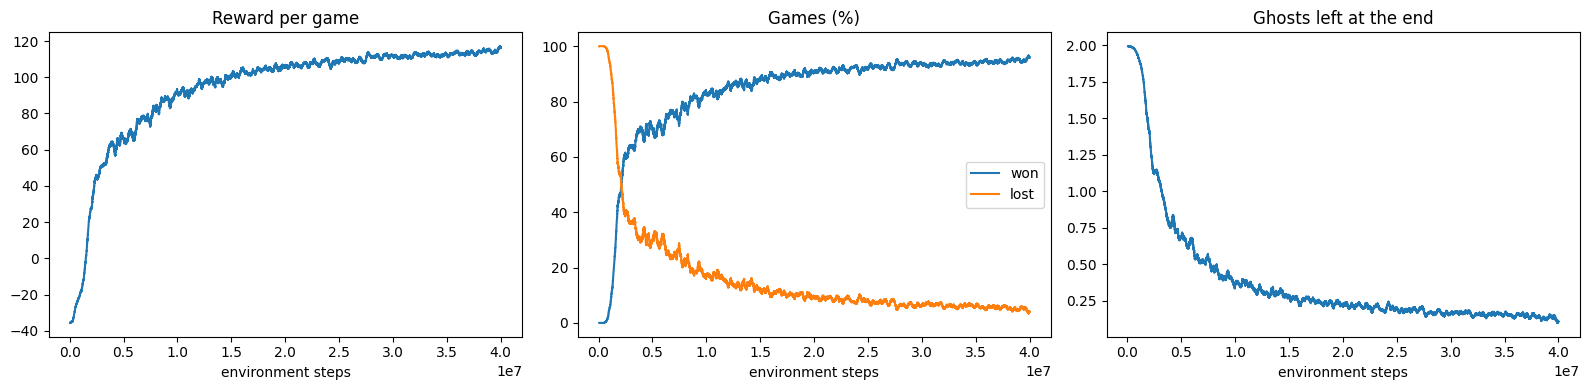
\includegraphics[width=\textwidth]{../Media/a2c_ppo_training.png}
  \caption{Training of the agent \code{Trainings/A2C/PPO\_1} on a Kaggle
    GPU, game \code{v1}: reward per game, games won and lost, and ghosts
    left at the end, against the number of environment steps (averages
    over $2000$ games).}
  \label{fig:ppo-training}
\end{figure}

\begin{pacman}{From $79\%$ to $97\%$}{ppo-results}
  \cref{fig:ppo-training} shows the training of the PPO agent over $40$
  million steps. The agent wins about half of its games after $2$ million
  steps, $80\%$ after $10$ million, and about $95\%$ at the end, while the
  number of ghosts left at the end falls from $2$ to about $0.1$. Evaluated
  on $1000$ games:
  \begin{center}
    \begin{tabular}{@{}lcc@{}}
      \toprule
      & Original A2C & PPO agent (\code{PPO\_1}) \\
      \midrule
      Games won & $79.4\%$ & $96.6\%$ \\
      Games ending with no ghost left & $51.4\%$ & $93.6\%$ \\
      Games with both power cookies eaten & $83.4\%$ & $96.8\%$ \\
      Average number of ghosts left & $0.69$ & $0.095$ \\
      \bottomrule
    \end{tabular}
  \end{center}
  The original A2C agent of the repository used a stride-$2$ network on a
  single RGB image, $n$-step returns and one gradient step per batch. The
  PPO agent differs in several ways at once: feature planes and two
  frames, a full-resolution symmetric network, GAE, PPO updates, a
  curriculum and a larger entropy bonus. Since all were changed together,
  the experiment does not tell how much each one contributes; it shows that
  together they divide the losing rate by six.
\end{pacman}

\section{Summary}

\begin{itemize}[nosep]
  \item The performance difference lemma measures a new policy with the
    advantages of the old one; with importance sampling it gives a
    surrogate objective that can be estimated from the old policy's data
    and agrees with $J$ to first order.
  \item PPO maximises a clipped version of the surrogate, a pessimistic
    bound that removes the incentive to change the probability of an
    action by more than a factor $1 \pm \epsilon$; this allows several
    epochs of mini-batch updates on each batch. A2C is the case of a single
    step.
  \item The KL estimator $(\rho - 1) - \log \rho$ and the clip fraction
    monitor the size of the updates.
  \item On Pacman, PPO with a better input and network wins $96.6\%$ of the
    games, against $79.4\%$ for the original A2C agent.
\end{itemize}

\chapter{Continuous actions: DDPG, TD3 and SAC}
\label{ch:continuous}

In robotics and control the actions are vectors of real numbers (torques,
forces, steering angles). Pacman's five moves are not, so this chapter uses
the classical continuous control benchmarks: swinging up a pendulum,
making a simulated robot walk (the MuJoCo tasks). Policy gradients with
Gaussian policies (\cref{sec:gaussian}) work there, and PPO is a standard
baseline; but they are on-policy and need many samples. The algorithms of
this chapter are \emph{off-policy actor-critic} methods: like DQN they learn
a Q-function from a replay memory, and they replace the maximisation over
actions, impossible on a continuum, by a learnt actor.

\section{Deterministic policy gradients}

Let $\mu_\theta : \States \to \R^k$ be a deterministic policy and $Q^\mu$ its
action-value function. The idea of DDPG is to move the action
$\mu_\theta(s)$ in the direction that increases $Q^\mu(s, \cdot)$.

\begin{theorem}{Deterministic policy gradient (stated without proof)}{dpg}
  Under regularity conditions (Silver et al., 2014), with $J(\theta) =
  \E[\sum_t \gamma^t R_{t+1}]$ for the policy $\mu_\theta$ and $\rho^\mu$ its
  discounted state distribution,
  \begin{equation}
    \label{eq:dpg}
    \nabla_\theta J(\theta) = \E_{s \sim \rho^\mu}\left[ \nabla_\theta
    \mu_\theta(s)\, \nabla_a Q^\mu(s, a) \big|_{a = \mu_\theta(s)}
    \right].
  \end{equation}
\end{theorem}

The formula is the chain rule applied to $Q^\mu(s, \mu_\theta(s))$, with the
remarkable fact (as in the stochastic policy gradient theorem) that the
effect of $\theta$ on the state distribution does not appear. It is also
the limit of the stochastic policy gradient for Gaussian policies whose
variance tends to $0$. Since the gradient involves no expectation over
actions, it can be estimated from states drawn from a replay memory filled
by an exploratory policy: the deterministic policy gradient is naturally
off-policy.

\section{DDPG}

Deep deterministic policy gradient (DDPG, Lillicrap et al., 2016) is
``DQN for continuous actions''. A critic $Q_\phi$ is trained with the
Bellman target of the deterministic policy, using target networks for both
the critic and the actor:
\begin{equation}
  y = r + \gamma (1 - d)\, Q_{\phi^-}\!\left(s', \mu_{\theta^-}(s')\right),
\end{equation}
and the actor follows \eqref{eq:dpg} with the critic in place of $Q^\mu$:
it maximises $\E_s[Q_\phi(s, \mu_\theta(s))]$ by gradient ascent through the
critic. Exploration adds noise to the actions (Gaussian, or an
Ornstein--Uhlenbeck process in the original paper), and the target networks
are updated by Polyak averaging. DDPG works but is brittle: the actor
exploits the errors of the critic, seeking actions where $Q_\phi$ is
overestimated, and the overestimation is propagated by the targets.

\section{TD3}

Twin delayed DDPG (TD3, Fujimoto et al., 2018) adds three corrections.
\begin{enumerate}
  \item \textbf{Clipped double Q-learning.} Two critics $Q_{\phi_1},
    Q_{\phi_2}$ are trained, and the target uses the smaller of their
    target versions:
    \begin{equation}
      y = r + \gamma (1 - d) \min_{i = 1, 2} Q_{\phi_i^-}(s', \tilde a'),
    \end{equation}
    a pessimistic estimate that counters the maximisation bias.
  \item \textbf{Target policy smoothing.} $\tilde a' = \mu_{\theta^-}(s') +
    \mathrm{clip}(\varepsilon, -c, c)$ with $\varepsilon \sim \mathcal{N}(0,
    \sigma^2)$: the target is averaged over nearby actions, so that a narrow
    peak of the critic cannot be exploited.
  \item \textbf{Delayed policy updates.} The actor and the target networks
    are updated once every two critic updates, so that the actor follows a
    critic that has had time to settle.
\end{enumerate}

\begin{proposition}{The minimum of two estimates is not optimistic}{td3-min}
  Let $Q_1 = q + \varepsilon_1$ and $Q_2 = q + \varepsilon_2$ be two
  estimates of a value $q$ with errors of mean zero. Then $\E[\min(Q_1,
  Q_2)] \leq q$, with strict inequality as soon as $\Prob(\varepsilon_1 \neq
  \varepsilon_2) > 0$.
\end{proposition}

\begin{proof}
  $\min(Q_1, Q_2) = \frac{Q_1 + Q_2}{2} - \frac{\abs{Q_1 - Q_2}}{2}$, whose
  expectation is $q - \frac{1}{2} \E\abs{\varepsilon_1 - \varepsilon_2}$.
\end{proof}

The bias is now downwards. An underestimated action is avoided by the
actor and is not explored further, which limits the damage, whereas an
overestimated one is sought and its error propagated: pessimism is the
safer error.

\section{Soft actor-critic}

Soft actor-critic (SAC, Haarnoja et al., 2018) learns a stochastic policy
that maximises the reward \emph{and} its own entropy.

\begin{definition}{Maximum entropy objective}{maxent}
  For a temperature $\alpha > 0$,
  \begin{equation}
    J_\alpha(\pi) = \E_\pi\left[ \sum_t \gamma^t \left( R_{t+1} + \alpha\,
    \mathcal{H}(\pi(\cdot \mid S_t)) \right) \right],
  \end{equation}
  where $\mathcal{H}(\pi(\cdot \mid s)) = -\E_{a \sim \pi(\cdot \mid s)}[\log
  \pi(a \mid s)]$. The \emph{soft} action values of $\pi$ satisfy
  \begin{equation}
    \label{eq:soft-bellman}
    Q^\pi(s, a) = r(s, a) + \gamma\, \E_{s'}\left[ V^\pi(s') \right],
    \qquad V^\pi(s) = \E_{a \sim \pi(\cdot \mid s)}\left[ Q^\pi(s, a) - \alpha
    \log \pi(a \mid s) \right].
  \end{equation}
\end{definition}

The entropy term rewards the policy for keeping several actions possible:
it explores by construction, it learns several ways of solving a task, and
it is more robust to perturbations. We prove the two steps of soft policy
iteration for finitely many actions (the continuous case is analogous with
densities).

\begin{proposition}{Soft policy evaluation}{soft-eval}
  For a fixed policy $\pi$, the operator $(\T^\pi_{\mathrm{soft}} Q)(s, a) =
  r(s, a) + \gamma\, \E_{s'} \E_{a' \sim \pi}[Q(s', a') - \alpha \log \pi(a'
  \mid s')]$ is a $\gamma$-contraction in the sup norm; its fixed point is
  the soft action-value function $Q^\pi$.
\end{proposition}

\begin{proof}
  The entropy terms do not depend on $Q$: they are an additional reward
  $r'(s, a) = -\alpha \gamma\, \E_{s'} \E_{a'}[\log \pi(a' \mid s')]$,
  bounded for finitely many actions. The operator is therefore the Bellman
  expectation operator for action values with reward $r + r'$, a
  $\gamma$-contraction (\cref{lem:contraction}).
\end{proof}

\begin{lemma}{Soft policy improvement}{soft-improvement}
  Let $\pi_{\mathrm{new}}(\cdot \mid s) \propto \exp(Q^{\pi}(s, \cdot) /
  \alpha)$ for every $s$ (the minimiser of $\mathrm{KL}(\pi'(\cdot \mid s)
  \,\|\, \exp(Q^\pi(s, \cdot)/\alpha) / Z(s))$). Then $Q^{\pi_{\mathrm{new}}}
  \geq Q^\pi$.
\end{lemma}

\begin{proof}
  For a fixed state $s$, let $f(\pi') = \E_{a \sim \pi'}[Q^\pi(s, a) - \alpha
  \log \pi'(a \mid s)]$. Writing $\pi^\star(a) = \exp(Q^\pi(s, a)/\alpha) /
  Z(s)$, we have $Q^\pi(s, a) = \alpha \log \pi^\star(a) + \alpha \log Z(s)$,
  hence $f(\pi') = \alpha \log Z(s) - \alpha\, \mathrm{KL}(\pi' \,\|\,
  \pi^\star)$, maximal at $\pi' = \pi^\star = \pi_{\mathrm{new}}(\cdot \mid
  s)$. In particular $f(\pi_{\mathrm{new}}) \geq f(\pi) = V^\pi(s)$. Then, as
  in the proof of \cref{thm:pi-improvement},
  \begin{align*}
    Q^\pi(s, a) &= r(s, a) + \gamma \E_{s'}[V^\pi(s')] \\
    &\leq r(s, a) + \gamma \E_{s'} \E_{a' \sim \pi_{\mathrm{new}}}
      \left[Q^\pi(s', a') - \alpha \log \pi_{\mathrm{new}}(a' \mid s')
      \right] = (\T^{\pi_{\mathrm{new}}}_{\mathrm{soft}} Q^\pi)(s, a),
  \end{align*}
  and iterating the monotone contraction $\T^{\pi_{\mathrm{new}}}_{\mathrm
  {soft}}$ gives $Q^\pi \leq Q^{\pi_{\mathrm{new}}}$.
\end{proof}

As $\alpha \to 0$, $\pi_{\mathrm{new}}$ concentrates on the greedy actions
and soft policy iteration becomes policy iteration. In practice:
\begin{itemize}
  \item two soft critics are trained (clipped double Q, as in TD3) towards
    $y = r + \gamma (1 - d) \left( \min_i Q_{\phi_i^-}(s', \tilde a') -
    \alpha \log \pi_\theta(\tilde a' \mid s') \right)$ with $\tilde a' \sim
    \pi_\theta(\cdot \mid s')$;
  \item the actor minimises $\E_{s} \E_{a \sim \pi_\theta}[\alpha \log
    \pi_\theta(a \mid s) - \min_i Q_{\phi_i}(s, a)]$, the KL divergence of
    the lemma up to a constant, using the \emph{reparametrisation trick}:
    $a = \tanh(\mu_\theta(s) + \sigma_\theta(s) \odot \xi)$ with $\xi \sim
    \mathcal{N}(0, I)$, so that gradients flow through the sampled action;
  \item the temperature is adjusted automatically so that the entropy of
    the policy stays near a target (for example $-k$ for $k$-dimensional
    actions), by gradient descent on $\alpha\, \E[-\log \pi(a \mid s) -
    \bar{\mathcal{H}}]$.
\end{itemize}

\begin{proposition}{Density of a squashed Gaussian}{tanh-density}
  If $u \in \R^k$ has density $\nu$ and $a = \tanh(u)$ componentwise, then
  \begin{equation}
    \log \pi(a) = \log \nu(u) - \sum_{i=1}^{k} \log\left(1 - \tanh^2
    (u_i)\right).
  \end{equation}
\end{proposition}

\begin{proof}
  The map $u \mapsto \tanh(u)$ is a bijection from $\R^k$ to $(-1, 1)^k$
  with diagonal Jacobian of entries $1 - \tanh^2(u_i) > 0$. By the change of
  variables formula, $\pi(a) = \nu(u) / \prod_i (1 - \tanh^2(u_i))$.
\end{proof}

SAC is sample-efficient, stable across hyperparameters, and one of the
standard algorithms for continuous control; a discrete-action variant also
exists, in which the expectations over actions are computed exactly.

\section{Summary}

\begin{itemize}[nosep]
  \item With continuous actions, a learnt actor replaces the maximisation
    over actions; the deterministic policy gradient moves the action along
    the gradient of the critic, and is naturally off-policy.
  \item DDPG is DQN for continuous actions; TD3 makes it reliable with
    clipped double critics (a downward bias, the safer one), target policy
    smoothing and delayed actor updates.
  \item SAC maximises reward plus entropy; soft policy evaluation and
    improvement mirror their classical versions, and with the
    reparametrisation trick and automatic temperature it is a robust
    default for continuous control.
\end{itemize}

\chapter{Model-based reinforcement learning and planning}
\label{ch:model-based}
\label{ch:search}

Model-free methods learn values or policies directly from experience.
Model-based methods also use a \emph{model} of the environment, given or
learnt, to \emph{plan}: to compute what to do by simulating rather than by
acting. Planning can happen in the background, generating simulated
experience to train the values or the policy (Dyna, MBPO), or at decision
time, searching from the current state before each move (rollouts, MCTS,
AlphaZero, MuZero). This chapter covers both, then returns to Pacman: the
look-ahead search of the repository, the question of what the search may
know about the ghosts, and expert iteration, which teaches the search's
decisions back to the network.

\section{Models and background planning}

A \emph{model} predicts the next state and reward, $\hat p(s', r \mid s,
a)$, either as a distribution or as a sampler. It can be known (the rules
of a board game, a physics simulator, a copy of the Pacman environment) or
learnt from the transitions observed, by supervised learning.

\begin{algobox}{Dyna-Q (Sutton, 1990)}
  \begin{algorithmic}[1]
    \For{each real step}
      \State in state $s$, play $a$ ($\varepsilon$-greedy w.r.t.\ $Q$),
        observe $r, s'$
      \State Q-learning update with $(s, a, r, s')$
      \State model update: $\mathrm{Model}(s, a) \gets (r, s')$
      \For{$n$ planning steps}
        \State pick a previously visited $(\tilde s, \tilde a)$;
          $(\tilde r, \tilde s') \gets \mathrm{Model}(\tilde s, \tilde a)$
        \State Q-learning update with $(\tilde s, \tilde a, \tilde r,
          \tilde s')$
      \EndFor
    \EndFor
  \end{algorithmic}
\end{algobox}

Each real transition is reused through the model many times, propagating
values much faster than with Q-learning alone. \emph{Prioritised sweeping}
chooses the simulated updates where they matter: when a value changes, the
predecessors of the state are queued with a priority equal to the size of
the change they would undergo.

A learnt model is wrong, and planning amplifies its errors: the planner
seeks the actions whose predicted outcome is best, including those where
the model is optimistically wrong. The following lemma quantifies the
effect of model errors on values.

\begin{lemma}{Simulation lemma}{simulation}
  Let $M = (p, r)$ and $\hat M = (\hat p, \hat r)$ be two MDPs on the same
  states and actions with rewards bounded by $R_{\max}$, and suppose
  $\abs{r(s, a) - \hat r(s, a)} \leq \varepsilon_r$ and $\sum_{s'}
  \abs{p(s' \mid s, a) - \hat p(s' \mid s, a)} \leq \varepsilon_p$ for all
  $s, a$. Then for every policy $\pi$,
  \begin{equation}
    \norm{v^\pi_M - v^\pi_{\hat M}}_\infty \leq \frac{\varepsilon_r}{1 -
    \gamma} + \frac{\gamma\, \varepsilon_p\, R_{\max}}{(1 - \gamma)^2}.
  \end{equation}
\end{lemma}

\begin{proof}
  With the matrix notation of \cref{prop:matrix}, $v = r_\pi + \gamma P_\pi
  v$ and $\hat v = \hat r_\pi + \gamma \hat P_\pi \hat v$, so
  \begin{equation*}
    v - \hat v = (r_\pi - \hat r_\pi) + \gamma (P_\pi - \hat P_\pi) v +
    \gamma \hat P_\pi (v - \hat v).
  \end{equation*}
  Each row of $P_\pi - \hat P_\pi$ has $\ell_1$ norm at most
  $\varepsilon_p$ and $\norm{v}_\infty \leq R_{\max} / (1 - \gamma)$
  (\cref{prop:return-props}), and $\hat P_\pi$ is stochastic. Taking sup
  norms, $\norm{v - \hat v}_\infty \leq \varepsilon_r + \gamma
  \varepsilon_p R_{\max} / (1 - \gamma) + \gamma \norm{v - \hat
  v}_\infty$; solve.
\end{proof}

\begin{intuition}
  A model that is wrong about the rewards by $\varepsilon_r$ makes that
  error at every simulated step, hence $\varepsilon_r / (1 - \gamma)$ over
  the horizon. A model that is wrong about the transitions is worse: at
  each step it sends the simulation to slightly wrong states, and landing
  in the wrong place can cost as much as the whole range of values,
  $R_{\max} / (1 - \gamma)$; this too happens at every step, hence the
  square. Imagined trajectories drift away from reality the longer they
  run.
\end{intuition}

The factor $1 / (1 - \gamma)^2$ reflects the compounding of errors over
long simulated trajectories. Modern methods therefore keep the simulated
trajectories short: MBPO (Janner et al., 2019) branches rollouts of a few
steps from real states with an ensemble of learnt models, and trains SAC
on the mixture of real and simulated transitions. World-model methods
(Dreamer, Hafner et al., 2020--2023) learn a latent dynamics model from
images and train an actor-critic entirely in imagination.

\section{Decision-time planning}

Background planning improves the policy everywhere; decision-time planning
concentrates the computation on the current state. It is how game-playing
programs have always worked, and it pays off when the policy alone is
imperfect: a trained policy decides each move in one glance at the board,
and when the PPO agent of \cref{ch:ppo} loses, it is usually because it
walks into a trap that only closes a few moves later.

\subsection{Rollouts}

Suppose we can simulate the game from the current state: here, a copy of
the environment (\code{PacmanEnvironment.clone()}). To evaluate a move $a$
in state $s$, play $a$ in a copy, then let a \emph{rollout policy} $\pi$
play for at most $H$ moves, and score the simulation by
\begin{equation}
  \label{eq:rollout-return}
  \hat G = \sum_{k=0}^{m-1} \gamma^k R_{k+1} + \gamma^m\, V(S_m),
\end{equation}
where $m \leq H + 1$ is the number of moves simulated and $V(S_m) = 0$ if
the game ended. Averaging $N$ independent simulations gives an estimate
$\hat q(s, a)$.

\begin{proposition}{What a rollout estimates}{rollout}
  If $V = v_\pi$, then $\E[\hat G] = q_\pi(s, a)$ for every horizon $H$,
  and the average of $N$ independent simulations has variance
  $\mathrm{Var}(\hat G) / N$. Playing in $s$ an action maximising $q_\pi(s,
  \cdot)$, and following $\pi$ afterwards, is at least as good as $\pi$.
\end{proposition}

\begin{proof}
  $\E[\hat G]$ is $(\T^\pi)^{H} V$ applied after the first move, as in
  \cref{prop:nstep-error}; with $V = v_\pi$ every application of $\T^\pi$
  leaves $v_\pi$ unchanged, so $\E[\hat G] = \E[R_1 + \gamma v_\pi(S_1)
  \mid s, a] = q_\pi(s, a)$. The variance of a mean of $N$ independent
  copies is the variance divided by $N$. The last claim is the policy
  improvement theorem (\cref{cor:greedy-improvement}) applied in the single
  state $s$.
\end{proof}

In the repository the rollout policy is the trained agent itself (greedy
moves), and $V$ its value head; the rollouts therefore estimate what
happens if the agent plays $a$ and then goes on as usual.

\paragraph{Common random numbers.} The moves of the ghosts are random. To
compare two candidate moves, the $k$-th simulation of each move uses the
same random numbers. For two estimates $X$ and $Y$,
\begin{equation}
  \mathrm{Var}(X - Y) = \mathrm{Var}(X) + \mathrm{Var}(Y) - 2\,
  \mathrm{Cov}(X, Y),
\end{equation}
and simulations that share the ghosts' random draws are positively
correlated, so their \emph{difference}, which decides the move, is much
less noisy than each of them.

\subsection{Two ways of choosing the move}

\begin{definition}{Value mode and safety mode}{search-modes}
  Let $M$ be the set of candidate moves (the moves leading to different
  cells), $a_0$ the agent's move, and, for each $a \in M$, $\hat q(a)$ the
  average score and $\hat d(a)$ the fraction of its $N$ simulations in
  which Pacman dies.
  \begin{itemize}[nosep]
    \item \emph{Value mode:} play $\argmax_{a \in M} \hat q(a)$.
    \item \emph{Safety mode:} keep $a_0$ unless $\hat d(a_0) - \min_a \hat
      d(a) \geq \kappa$; otherwise play, among the moves of minimal death
      rate, the one of best average score. The repository uses $\kappa =
      0.15$.
  \end{itemize}
  The search is only used when a ghost is at most $5$ cells away
  (Manhattan distance), about $33$ moves per game.
\end{definition}

\begin{pacman}{Why the value mode fails}{value-mode}
  With $N = 20$ simulations, the value mode \emph{lowered} the win rate
  (about $95.5\%$, against $96.1\%$ without search) and changed about a
  quarter of the agent's moves. The reason is noise: the returns of a
  simulation range from $-35$ (death) to $+20$ and more (a ghost eaten),
  so the standard deviation of a mean of $20$ of them is of the order of
  a few points, while the difference in value between two reasonable moves
  is often a fraction of a point. The maximum of noisy estimates then picks
  a random move (\cref{prop:max-bias}). The death rate is a much more
  robust signal: a trap shows up as many deaths for one move and few for
  another. The safety mode changes the agent's move about $0.6$ times per
  game, only when it clearly walks into a trap.
\end{pacman}

\begin{intuition}
  The safety mode does not ask the search which move is best, a question
  its $20$ noisy simulations per move cannot answer reliably. It asks a
  simpler one: is the move the agent wants to play clearly more dangerous
  than another? The trained policy keeps the initiative, and the search
  acts as a safety net that vetoes a move only when the evidence is strong.
\end{intuition}

\begin{lstlisting}[caption={Choosing the move (\code{pacman\_search.py},
  \code{LookaheadSearch.select\_action}, excerpt)}]
scores = {m: np.mean([s["score"] for s in sims if s["move"] == m])
          for m in moves}
if self.mode == "value":
    best = max(moves, key=lambda m: scores[m])
    if scores[agent_move] >= scores[best] - 1e-9:
        return agent_action
else:  # safety mode
    deaths = {m: np.mean([s["env"].dead for s in sims
                          if s["move"] == m]) for m in moves}
    safest = min(deaths.values())
    if deaths[agent_move] - safest < self.margin:   # kappa = 0.15
        return agent_action
    best = max((m for m in moves if deaths[m] == safest),
               key=lambda m: scores[m])
return best
\end{lstlisting}

\section{Monte Carlo tree search}

The search of the repository is the simplest form of Monte Carlo planning:
a tree of depth one with the same number of simulations for every move.
Monte Carlo tree search (MCTS) grows a deeper tree, asymmetrically, and
allocates the simulations to the moves that deserve them. Each node of the
tree stores, for each action, a visit count $N(s, a)$ and a mean value
$\hat q(s, a)$.

\begin{algobox}{Monte Carlo tree search (one simulation)}
  \begin{algorithmic}[1]
    \State \textbf{selection:} from the root, descend the tree choosing at
      each node the action maximising a selection rule (UCT below), until a
      leaf
    \State \textbf{expansion:} add one child of the leaf to the tree
    \State \textbf{evaluation:} estimate the value of the new node, by a
      rollout with a default policy, or by a value network
    \State \textbf{backup:} along the path, increment $N(s, a)$ and update
      $\hat q(s, a)$ with the observed return
  \end{algorithmic}
\end{algobox}

After the simulations, the move played is the most visited action of the
root. The UCT selection rule (Kocsis and Szepesv\'ari, 2006) treats each
node as a bandit and applies UCB1 (\cref{def:ucb1}):
\begin{equation}
  a = \argmax_{a} \left( \hat q(s, a) + c \sqrt{\frac{\ln N(s)}{N(s,
  a)}} \right),
\end{equation}
with $N(s) = \sum_a N(s, a)$. Kocsis and Szepesv\'ari proved that, with
suitable $c$, the probability of choosing a wrong move at the root tends
to $0$ as the number of simulations grows. In a stochastic game such as
Pacman, the tree is built over sequences of the agent's moves
(``open-loop'' MCTS), each simulation replaying the sequence on a fresh
copy of the game, or the tree also branches on chance outcomes.

\begin{intuition}
  MCTS places a bandit at every node of the tree. Moves that look good are
  simulated more and their subtrees grow deeper; moves that look bad are
  revisited only now and then, in case their first results were unlucky.
  The tree grows towards the promising lines, as a chess player analyses
  the critical variations deeply and dismisses the others after a glance.
\end{intuition}

\begin{remark}{MCTS for two-player games}{mcts-two-players}
  In a game between two opponents, such as Hex, chess or Go, the players
  alternate along each path of the tree, and the statistics of a node are
  kept from the point of view of the player who made the move leading to
  it. During the backup the result is therefore flipped at each level: a
  win for one player is a loss for the other. Each player then selects,
  with UCT, the moves that are best \emph{for itself}, which is the minimax
  principle obtained by sampling. The move finally played can be the most
  visited child of the root (the usual, most robust choice), the child with
  the highest mean value (optimistic when it has few visits), or the child
  with the highest lower confidence bound (pessimistic).

  A C++ implementation for Hex, with brute force, flat Monte Carlo and MCTS
  players, and a step-by-step account of the algorithm on a small example,
  is in the repository
  \href{https://github.com/CL-BZH/Hex_game_AI}{CL-BZH/Hex\_game\_AI}
  (\code{hex\_machine\_mcts.h} and \code{Docs/mcts.pdf}). The
  \href{https://CL-BZH.github.io/MCTS-Visualizer/}{MCTS Visualizer}
  (repository
  \href{https://github.com/CL-BZH/MCTS-Visualizer}{CL-BZH/MCTS-Visualizer})
  shows the tree growing iteration by iteration on a simple two-player game,
  with the four phases and the UCB1 values of each node.
\end{remark}

\subsection{AlphaZero}

AlphaZero (Silver et al., 2018) learnt chess, shogi and Go from the rules
alone by combining MCTS with a network $f_\theta(s) = (\mathbf{p}, v)$ that
outputs a prior policy and a value. MCTS uses them through the PUCT rule
\begin{equation}
  a = \argmax_a \left( \hat q(s, a) + c\, p_a(s) \frac{\sqrt{N(s)}}{1 +
  N(s, a)} \right),
\end{equation}
which explores first the moves the network finds promising, and evaluates
the leaves with $v$ instead of rollouts. The games of self-play provide the
training data: the network is trained to predict the visit distribution of
the search, $\boldsymbol{\pi}_t \propto N(s_t, \cdot)$, and the final
result $z$ of the game,
\begin{equation}
  \ell(\theta) = (z - v)^2 - \boldsymbol{\pi}_t^\top \log \mathbf{p} + c
  \norm{\theta}^2.
\end{equation}
The search is a \emph{policy improvement operator}: its visit distribution
is better than the prior it started from, and training the network on it
is \emph{expert iteration} (Anthony et al., 2017). The network then makes
the next searches better, and so on.

\begin{intuition}
  In PUCT the prior $p_a(s)$ plays the role of intuition: the moves the
  network likes are explored first, and the bonus, decreasing like $1 /
  (1 + N(s, a))$, lets the search's own statistics take over as they
  accumulate. In the loss, the value head learns to predict who wins, and
  the policy head learns to imitate the search, which plays better than
  the raw network because it looks ahead. The program pulls itself up: a
  better network makes a better search, which makes a better teacher.
\end{intuition}

\subsection{MuZero}

MuZero (Schrittwieser et al., 2020) plans without knowing the rules. It
learns three functions: a representation $h$ mapping observations to a
latent state, a dynamics function $g(z, a) = (\hat r, z')$, and a
prediction function $f(z) = (\mathbf{p}, v)$. The latent model is not trained
to reconstruct observations, only to predict, along real trajectories
unrolled for a few steps, the rewards, the values and the search policies:
it models only what matters for planning. MuZero matched AlphaZero in board
games and set the state of the art on Atari at the time.

\section{What does the search know about the ghosts?}

A copy of the environment simulates the ghosts with the game's own code,
which the agent never sees. Using it would give the search a \emph{perfect
model} of the opponents: legitimate in a board game whose rules are known,
debatable for Pacman, where the behaviour of the ghosts is part of what the
agent should discover. The search therefore offers three \emph{ghost
models}:
\begin{itemize}[nosep]
  \item \code{exact}: the game's code (perfect model), used only as a
    reference;
  \item \code{chase} (default): worst case; when Pacman has no power each
    ghost moves along a shortest path towards him, and randomly when he has
    power;
  \item \code{estimated}: a ghost chases with probability $p_{\mathrm{chase}}$
    and moves randomly otherwise; when Pacman has power it moves away from
    him with probability $p_{\mathrm{flee}}$. Both probabilities are
    estimated for each ghost from its observed moves.
\end{itemize}
With \code{chase} and \code{estimated}, the search uses only what the agent
observes (positions, power) and the rules for Pacman himself.

\begin{proposition}{Estimating a ghost's chase probability}{ghost-estimator}
  Model each observed move of a ghost as: towards Pacman with probability
  $p$, otherwise uniform among its $n$ reachable cells, of which $m$ go
  towards Pacman ($0 < m < n$). Then the probability that the move goes
  towards Pacman is $p + (1 - p)\, m / n$, and after observing moves with
  ratios $q_i = m_i / n_i$ the posterior density of $p$ under a prior
  $\mathrm{Beta}(2, 2)$ is proportional to
  \begin{equation}
    p (1 - p) \prod_{i \in \mathcal{T}} \left( p + (1 - p) q_i \right)
    \prod_{i \notin \mathcal{T}} (1 - p)(1 - q_i),
  \end{equation}
  where $\mathcal{T}$ is the set of moves that went towards Pacman.
\end{proposition}

\begin{proof}
  A move goes towards Pacman either because the ghost chases (probability
  $p$) or because it moves randomly (probability $1 - p$) and picks one of
  the $m$ cells out of $n$. The moves are independent given $p$, and the
  posterior is the prior density $\propto p(1 - p)$ times the likelihood.
\end{proof}

\begin{intuition}
  A move towards Pacman is evidence that the ghost chases, but weak
  evidence when most of the ghost's possible moves go towards Pacman anyway
  ($q_i$ close to $1$): a random ghost would have done the same. A move
  away from Pacman is strong evidence of randomness, since a chasing ghost
  never makes it. The posterior weighs each observation by how much it
  discriminates between the two behaviours.
\end{intuition}

The repository takes the maximum of this posterior on a grid. Over many
games, it recovers $p \approx 0.73$ and $0.64$ for the two ghosts (their
configured aggressiveness is $0.74$ and $0.64$), and a flee probability of
about $0.08$: edible ghosts move almost at random. The first version of
the models assumed that edible ghosts always flee; the simulated hunts then
failed, the search judged eating a ghost dangerous and made the agent
hesitate in front of an edible ghost. Estimating the flee probability
fixed it: a model that is wrong in the optimistic or the pessimistic
direction can both mislead a planner.

\begin{pacman}{The search on 1000 games}{search-results}
  With $20$ simulations, horizon $15$, safety mode, the search was
  evaluated on $1000$ games: all the games lost without search, and a
  sample of the won ones, were replayed with search from the same starting
  conditions.
  \begin{center}
    \begin{tabular}{@{}lc@{}}
      \toprule
      Ghost model & Estimated win rate \\
      \midrule
      no search & $96.1\%$ \\
      \code{exact} & $97.1\% \pm 0.5$ \\
      \code{chase} & $97.5\% \pm 0.5$ \\
      \code{estimated} & $97.7\% \pm 0.3$ \\
      \bottomrule
    \end{tabular}
  \end{center}
  The models that do not know the ghosts' code do at least as well as the
  exact one: the gain comes from seeing a trap a few moves ahead, not from
  knowing the opponents' rules.
\end{pacman}

\section{Expert iteration}

The search is expensive (up to about $100$ simulated games per searched
move). If
the network could learn to make the search's decisions by itself, the gain
would be free at play time. Simply training the network on games played
\emph{by the search} (behaviour cloning) has a known flaw: the network only
sees the situations that the search gets into, and when it makes a mistake
of its own, it reaches situations it has never seen, where its errors
compound (Ross and Bagnell, 2010). The remedy, DAgger (Ross, Gordon and
Bagnell, 2011), lets the \emph{learner} play and asks the \emph{expert}
what it would have done in the situations the learner reached.

\begin{algobox}{Expert iteration (DAgger form), \code{pacman\_expert.py}}
  \begin{algorithmic}[1]
    \State start from the PPO agent $\pi_\theta$
    \For{each iteration}
      \State the agent plays $2000$ games alone; whenever a ghost is close,
        record the state $s$ and the search's move $a^\star(s)$
      \State record also a fraction of the other states, labelled with the
        agent's own move, and the discounted returns observed
      \State train on the data of the last iterations: weighted
        cross-entropy $-w(s) \log \pi_\theta(a^\star(s) \mid s)$ with
        $w(s) = 10$ where the search disagreed with the agent and $1$
        otherwise, and squared error of the value head
    \EndFor
  \end{algorithmic}
\end{algobox}

The labels of the states where the search agrees with the agent keep the
rest of its behaviour unchanged; the weight $10$ makes the few
disagreements count. Because the games are played by the agent alone,
each iteration also measures its progress.

\begin{pacman}{Results of expert iteration}{expert-results}
  Ten iterations of $2000$ games on Kaggle (search with $10$ simulations,
  horizon $10$, \code{chase} model), about one hour each, almost all of it
  spent in the search (on CPU). The search disagreed with the agent
  $0.27$ times per game at the first iteration and $0.12$ at the last, and
  the network reproduced $76\%$ of the corrections of its training data.
  On the same $1000$ games:
  \begin{center}
    \begin{tabular}{@{}lcc@{}}
      \toprule
      Same $1000$ games & Without search & With search ($20$) \\
      \midrule
      PPO agent (\code{PPO\_1}) & $97.1\%$ & $98.1\%$ \\
      After expert iteration (\code{Expert\_1}) & $97.7\%$ & $97.9\%$ \\
      \bottomrule
    \end{tabular}
  \end{center}
  Expert iteration and the search correct the same mistakes: without
  search the expert agent recovers about $60\%$ of the search's gain (and
  no longer loses games by the ``off-by-one'' of \cref{sec:game}), but with
  the search both agents reach about $98\%$.
\end{pacman}

\section{What is left?}

The repository classifies the lost games by cause (\code{pacman\_play.py}).
For the PPO agent alone, out of about $38$ losses in $1000$ games, $2$ come
from the off-by-one, $1$ from a ghost catching Pacman just after his power
ended, $6$ from \emph{bad starts} (Pacman caught in the first five moves),
and the others from traps. With the search, the same three bad starts are
lost in every configuration, which suggests that they cannot be won. The
$15$ to $18$ remaining losses resist both the search and expert iteration:
they are probably traps from which the agent's own policy, which plays the
simulations, cannot escape either. Going further would require a deeper
search (MCTS), or, following AlphaZero, alternating the improvement of the
search and of the network over many more iterations.

\section{Summary}

\begin{itemize}[nosep]
  \item A model can be used to generate simulated experience (Dyna, MBPO,
    Dreamer) or to search at decision time (rollouts, MCTS); the errors of
    a learnt model compound with the length of the simulations.
  \item MCTS treats each node as a bandit (UCT); AlphaZero guides it with a
    policy and value network and trains the network on the search's
    decisions; MuZero learns a latent model for planning.
  \item On Pacman, a depth-one search with a safety rule raises the win
    rate from $96\%$ to about $98\%$, without knowing the ghosts' code;
    expert iteration transfers part of this gain to the network alone.
\end{itemize}

\chapter[Imitation learning and offline RL]{Imitation learning and offline
  reinforcement learning}
\label{ch:imitation}

The previous chapters assumed that the agent learns by interacting with the
environment and receiving rewards. In many applications this is expensive
or dangerous (a car, a patient, a power grid), and the reward is hard to
write down, while \emph{data} are available: demonstrations by an expert,
or logs of past decisions. This chapter studies two ways of using them.
\emph{Imitation learning} learns from demonstrations, without rewards;
\emph{offline reinforcement learning} learns from a fixed dataset of
transitions with rewards, without further interaction.

\section{Behaviour cloning}

The simplest approach treats demonstrations $\mathcal{D} = \{(s_i, a_i)\}$
of an expert policy $\pi^\star$ as a supervised learning problem: fit
$\pi_\theta$ by maximum likelihood,
\begin{equation}
  \min_\theta\; \E_{(s, a) \sim \mathcal{D}}\left[ -\log \pi_\theta(a \mid
  s) \right].
\end{equation}
Behaviour cloning (BC) is simple and often works well with enough data
(it was used to drive a car as early as 1989, by ALVINN). Its weakness is
that the states of the training set are those visited by the expert. When
the learner makes a mistake, it reaches states the expert never visited,
where it has no data and makes more mistakes: the errors compound.

\begin{theorem}{Compounding errors of behaviour cloning}{bc}
  Consider episodes of $T$ steps with costs $c(s, a) \in [0, 1]$, a
  deterministic expert $\pi^\star$, and let $J(\pi)$ be the expected total
  cost of $\pi$. Let $d_t$ be the distribution of the expert's state at step
  $t$, and suppose that the learner $\pi$ disagrees with the expert with
  probability at most $\varepsilon$ on these distributions:
  $\Prob_{s \sim d_t,\, a \sim \pi(\cdot \mid s)}(a \neq \pi^\star(s)) \leq
  \varepsilon$ for all $t$. Then
  \begin{equation}
    J(\pi) \leq J(\pi^\star) + \varepsilon\, T^2.
  \end{equation}
\end{theorem}

\begin{proof}
  Run the expert and the learner with the same random numbers for the
  environment, so that their trajectories coincide as long as their actions
  coincide. Let $D_t$ be the event that the trajectories have diverged at
  or before step $t$. If they have not diverged before step $t$, the shared
  state is the expert's state, distributed as $d_t$, so the probability of
  a first disagreement at step $t$ is at most $\varepsilon$, and $\Prob(D_t)
  \leq t \varepsilon$. At step $t$ the costs of the two trajectories are
  equal outside $D_t$ and differ by at most $1$ on $D_t$. Summing,
  $J(\pi) - J(\pi^\star) \leq \sum_{t=1}^T t\varepsilon \leq \varepsilon
  T^2$.
\end{proof}

\begin{intuition}
  A learner who has only watched an expert drive has never seen the car
  on the shoulder of the road. After a small mistake it is in a situation
  it never trained on, where it makes more mistakes, and it may never
  return to familiar ground. A mistake at step $t$ can spoil all the
  remaining steps, so the cost of a per-step error rate $\varepsilon$ is
  multiplied by the horizon \emph{twice}.
\end{intuition}

The bound is tight up to constants: there are problems where a single
mistake leads to states from which the learner never recovers, and the
cost is then of order $\varepsilon T^2$, not the $\varepsilon T$ of a
supervised learning error accumulated over $T$ steps.

\section{DAgger}

The cure is to train the learner on the states \emph{it} visits. DAgger
(dataset aggregation, Ross, Gordon and Bagnell, 2011) requires an expert
that can be queried in any state.

\begin{algobox}{DAgger}
  \begin{algorithmic}[1]
    \State $\mathcal{D} \gets$ demonstrations of the expert; train
      $\pi_1$ on $\mathcal{D}$
    \For{$i = 1, 2, \dots, N$}
      \State run $\pi_i$ (optionally mixed with the expert) to collect states
        $s$
      \State ask the expert for its actions $\pi^\star(s)$; $\mathcal{D}
        \gets \mathcal{D} \cup \{(s, \pi^\star(s))\}$
      \State train $\pi_{i+1}$ on $\mathcal{D}$
    \EndFor
  \end{algorithmic}
\end{algobox}

DAgger is an online learning algorithm in disguise: training on the
aggregated data is ``follow the leader'' on the sequence of losses defined
by the learner's own state distributions. Ross et al.\ show, with a
no-regret learner, that some policy of the sequence has a cost $J(\pi) \leq
J(\pi^\star) + u\, T \varepsilon_N + o(1)$, where $\varepsilon_N$ is the
best training error on the aggregated data and $u$ bounds the increase of
the expert's cost-to-go after one wrong action: the error grows linearly in
$T$ when the expert can recover from the learner's mistakes.

\begin{intuition}
  DAgger is a driving instructor in the passenger seat: the learner
  drives, and in the situations \emph{it} gets into, including those
  caused by its own mistakes, the instructor says what it should have
  done. The training data then cover the states the learner actually
  visits, and the learner learns how to recover.
\end{intuition}

\begin{pacman}{Expert iteration is DAgger}{dagger}
  In \cref{ch:model-based}, the expert is the look-ahead search and the
  learner the PPO network: \code{pacman\_expert.py} lets the network play
  and asks the search for its move in the states the network reached, which
  is DAgger. The search can be queried in any state because it only needs
  a copy of the game. Training on games played \emph{by the search} would
  have been behaviour cloning, exposed to \cref{thm:bc}.
\end{pacman}

\section{Inverse reinforcement learning}

Behaviour cloning copies actions; inverse reinforcement learning (IRL)
recovers the \emph{reward} that the expert optimises, which transfers to new
dynamics and explains the behaviour. The problem is ill-posed: the reward
$r = 0$ makes every policy optimal, and adding to the reward a
\emph{shaping} term $\gamma \Phi(s') - \Phi(s)$, for any function $\Phi$,
changes the reward without changing the optimal policies (Ng, Harada and
Russell, 1999).
A principle is needed to choose among the rewards that explain the data.

\paragraph{Maximum entropy IRL.} Ziebart et al.\ (2008) take a linear
reward $r_\theta(\tau) = \theta^\top \phi(\tau)$ of the features $\phi(\tau)
= \sum_t \phi(s_t, a_t)$ of a trajectory, and model the expert as choosing
trajectories with probability $p_\theta(\tau) = \exp(\theta^\top
\phi(\tau)) / Z(\theta)$ (for deterministic dynamics): the maximum entropy
distribution that matches the feature expectations. The parameters are
fitted by maximum likelihood on the demonstrations.

\begin{proposition}{Gradient of maximum entropy IRL}{maxent-irl}
  The average log-likelihood $L(\theta) = \frac{1}{N} \sum_{i=1}^N \log
  p_\theta(\tau_i)$ of $N$ demonstrations is concave, with gradient
  \begin{equation}
    \nabla L(\theta) = \frac{1}{N} \sum_{i=1}^N \phi(\tau_i) -
    \E_{\tau \sim p_\theta}\left[ \phi(\tau) \right].
  \end{equation}
\end{proposition}

\begin{proof}
  $L(\theta) = \theta^\top \bar\phi - \log Z(\theta)$ with $\bar\phi$ the
  empirical mean of the features, and $\nabla \log Z(\theta) =
  \sum_\tau \phi(\tau) e^{\theta^\top \phi(\tau)} / Z(\theta) =
  \E_{p_\theta}[\phi]$. The Hessian of $\log Z$ is the covariance of $\phi$
  under $p_\theta$, positive semi-definite, so $L$ is concave.
\end{proof}

\begin{intuition}
  The gradient compares what the expert does with what the current model
  of the expert does. A feature the expert's trajectories show more often
  (staying far from the ghosts, say) gets a higher reward weight; a feature
  the model overproduces gets a lower one. Learning stops when the model's
  trajectories have the same feature statistics as the expert's.
\end{intuition}

At the optimum the model matches the expert's feature expectations. The
expectation under $p_\theta$ requires solving a soft (maximum entropy) RL
problem for the current reward, as in SAC (\cref{ch:continuous}): IRL is
an outer loop around RL, and therefore expensive.

\paragraph{Adversarial imitation.} GAIL (Ho and Ermon, 2016) skips the
reward: a discriminator $D_\psi(s, a)$ is trained to distinguish the
expert's pairs from the learner's, and the policy is trained by RL (TRPO or
PPO) with the reward $-\log(1 - D_\psi(s, a))$, so that it produces pairs
the discriminator takes for the expert's. As in generative adversarial
networks, at the equilibrium the occupancy measure of the learner matches
that of the expert (the procedure minimises their Jensen--Shannon
divergence). Unlike BC, GAIL matches distributions of states, not only
actions in the expert's states, and does not suffer from compounding
errors; but it needs interaction with the environment.

\section{Offline reinforcement learning}

In offline (or batch) RL, the agent receives a dataset $\mathcal{D} =
\{(s_i, a_i, r_i, s'_i)\}$ collected by one or several \emph{behaviour}
policies $\beta$, and must produce the best possible policy without
collecting more data. Q-learning and DQN are off-policy, so it is tempting
to run them on $\mathcal{D}$. This fails in practice, often badly.

\paragraph{Extrapolation error.} The target $r + \gamma \max_{a'} Q(s',
a')$ evaluates $Q$ at actions $a'$ that may never appear in the data for
$s'$. There the network's values are arbitrary, and the maximisation
selects precisely the actions whose values are overestimated. Online, the
agent would try these actions and correct the error; offline, nothing
corrects it, and the errors propagate through the targets. The
\emph{distribution shift} between the learnt policy and $\beta$ is the
central problem of offline RL. Three families of methods address it.

\paragraph{Policy constraints.} Keep the policy close to the behaviour
policy. BCQ (Fujimoto et al., 2019) only maximises over actions proposed by
a generative model of $\beta$. TD3+BC (Fujimoto and Gu, 2021) adds a
behaviour cloning term to the actor of TD3 (\cref{ch:continuous}):
\begin{equation}
  \max_\theta\; \E_{(s, a) \sim \mathcal{D}}\left[ \lambda\, Q_\phi(s,
  \mu_\theta(s)) - \norm{\mu_\theta(s) - a}^2 \right],
\end{equation}
a one-line change that is a strong baseline.

\paragraph{Conservative values.} CQL (Kumar et al., 2020) learns a
Q-function that underestimates the values of the actions absent from the
data. For discrete actions it adds to the TD loss the term
\begin{equation}
  \label{eq:cql}
  \alpha\, \E_{s \sim \mathcal{D}}\left[ \log \sum_{a} \exp Q(s, a) -
  \E_{a \sim \mathcal{D}(\cdot \mid s)}[Q(s, a)] \right],
\end{equation}
which pushes down the values of all actions (through a soft maximum) and
pushes up those of the actions in the data.

\begin{lstlisting}[caption={CQL loss for discrete actions (PyTorch)}]
q = q_net(states)                                  # (B, |A|)
q_data = q.gather(1, actions[:, None]).squeeze(1)  # Q(s, a), a in data
with torch.no_grad():
    target = rewards + gamma * (1 - dones) * \
        target_net(next_states).max(1).values
td_loss = F.smooth_l1_loss(q_data, target)
cql_loss = (torch.logsumexp(q, dim=1) - q_data).mean()
loss = td_loss + alpha * cql_loss
\end{lstlisting}

The following idealised, tabular version shows why the values become
conservative. Let $\mu(\cdot \mid s)$ be the policy whose values are pushed
down (in \eqref{eq:cql}, the softmax of $Q$), and consider the iteration
\begin{equation*}
  \hat Q_{k+1} = \argmin_Q\; \alpha \left( \E_{s, a \sim \mu} [Q(s, a)] -
  \E_{s, a \sim \beta}[Q(s, a)] \right) + \frac{1}{2} \E_{s, a \sim \beta}
  \left[ \left( Q(s, a) - (\T^\pi \hat Q_k)(s, a) \right)^2 \right],
\end{equation*}
where the states are drawn from the data and the pairs weighted by
$\beta(a \mid s) > 0$.

\begin{proposition}{CQL underestimates the value}{cql}
  The minimiser is $\hat Q_{k+1}(s, a) = (\T^\pi \hat Q_k)(s, a) - \alpha
  \left( \frac{\mu(a \mid s)}{\beta(a \mid s)} - 1 \right)$, and
  \begin{equation}
    \E_{a \sim \mu(\cdot \mid s)}\left[ \hat Q_{k+1}(s, a) \right] \leq
    \E_{a \sim \mu(\cdot \mid s)}\left[ (\T^\pi \hat Q_k)(s, a) \right].
  \end{equation}
\end{proposition}

\begin{proof}
  The objective separates over the pairs $(s, a)$. For one pair, the
  derivative with respect to $Q(s, a)$ is $\alpha (\mu(a \mid s) - \beta(a
  \mid s)) + \beta(a \mid s) (Q(s, a) - (\T^\pi \hat Q_k)(s, a))$ (up to
  the common factor of the state's weight); setting it to zero gives the
  minimiser. For the inequality, $\E_\mu[\mu / \beta - 1] = \sum_a \mu(a)^2
  / \beta(a) - 1 \geq 0$, by the Cauchy--Schwarz inequality $1 = (\sum_a
  \mu(a))^2 \leq \sum_a \mu(a)^2 / \beta(a) \cdot \sum_a \beta(a)$.
\end{proof}

The penalty is large where $\mu$ puts much more weight than the data:
exactly the actions whose values cannot be trusted.

\begin{intuition}
  CQL tells the Q-function: ``be pessimistic about what you have not
  seen''. An action that the policy would choose much more often than the
  data contain it gets its value pushed down, in proportion to that
  imbalance; actions well covered by the data are left almost unchanged.
  The policy then prefers actions whose good value is backed by evidence.
\end{intuition}

\paragraph{In-sample learning.} IQL (Kostrikov et al., 2022) never
evaluates $Q$ at actions outside the data. It fits $V(s)$ to an upper
expectile of $Q(s, a)$ over the actions of the data, minimising
$\E_{(s, a) \sim \mathcal{D}}[L_\tau(Q(s, a) - V(s))]$ with $L_\tau(u) =
\abs{\tau - \mathbb{1}(u < 0)}\, u^2$ and $\tau \approx 0.7$--$0.9$, which
approximates a maximum over the actions supported by the data; $Q$ is
fitted to $r + \gamma V(s')$; and the policy is extracted by
advantage-weighted regression, maximising $\E_{\mathcal{D}}[e^{b (Q(s, a) -
V(s))} \log \pi(a \mid s)]$: behaviour cloning weighted by the advantage.

\begin{intuition}
  An upper expectile of $Q(s, a)$ over the actions of the data is a soft
  version of ``the best action that was actually tried in this state''. IQL
  thus computes a maximum over the data's actions only, never asking the
  network about actions it has no data for, and then imitates the data,
  copying the good actions more than the bad ones.
\end{intuition}

\begin{remark}{Offline RL and Pacman}{offline-pacman}
  The replay memory of a DQN training run is an offline dataset of
  millions of transitions of Pacman. Running DQN on it from scratch, without
  interaction, is an instructive experiment: the values of the rare
  actions (walking into a ghost) are poorly constrained by the data, and
  the conservative loss above is a few lines to add to \code{DQN.learn}.
\end{remark}

\section{Summary}

\begin{itemize}[nosep]
  \item Behaviour cloning is supervised learning on demonstrations; its
    errors compound quadratically with the horizon, because the learner
    leaves the states covered by the data.
  \item DAgger queries the expert in the learner's own states and reduces
    the error to linear in the horizon; expert iteration with a search as
    expert is DAgger.
  \item Inverse RL recovers a reward (maximum entropy IRL matches feature
    expectations); GAIL matches occupancy measures adversarially.
  \item Offline RL suffers from extrapolation error at actions absent from
    the data; policy constraints (TD3+BC), conservative values (CQL) and
    in-sample learning (IQL) avoid it.
\end{itemize}

\chapter{Exploration}
\label{ch:exploration}

An agent learns only about what it tries. The bandits of \cref{ch:bandits}
showed the dilemma in its simplest form and the main answers: random
exploration ($\varepsilon$-greedy), optimism (UCB) and posterior sampling
(Thompson). In an MDP the dilemma is harder, because information is
delayed: reaching an informative state may take many deliberate steps, and
random actions rarely string them together. This chapter shows why, and
presents the methods that scale the bandit ideas to deep RL.

\section{Why dithering fails}

$\varepsilon$-greedy, Boltzmann exploration and the entropy bonus of PPO
are \emph{dithering} strategies: they perturb each action independently.
The following example, a ``combination lock'', shows that they can need a
time exponential in the size of the problem.

\begin{proposition}{Random exploration in a chain}{chain}
  Consider states $0, 1, \dots, n$, starting in $0$, where action
  \emph{right} moves from $k$ to $k + 1$ and action \emph{left} returns to
  $0$; the only reward is at state $n$. Under the uniform random policy,
  the expected number of steps to reach $n$ from $0$ is $2^{n+1} - 2$.
\end{proposition}

\begin{proof}
  Let $T_k$ be the expected number of steps to reach $n$ from $k$, so that
  $T_n = 0$ and $T_k = 1 + \frac{1}{2} T_{k+1} + \frac{1}{2} T_0$ for $k <
  n$. We show by induction that $T_k = T_0 - (2^{k+1} - 2)$. It holds for
  $k = 0$, and if it holds for $k$, then $T_{k+1} = 2 T_k - 2 - T_0 = T_0 -
  2^{k+2} + 2$. With $k = n$, $0 = T_0 - 2^{n+1} + 2$.
\end{proof}

A greedy agent with optimistic initial values solves the same chain in
$O(n^2)$ steps: every unvisited action looks attractive, so the agent
tries the actions of the states it reaches systematically. This is the
principle of the provably efficient algorithms.

\section{Optimism in the face of uncertainty}

\paragraph{Provably efficient exploration.} R-max (Brafman and
Tennenholtz, 2002) treats every state-action pair visited fewer than $m$
times as leading to a fictitious state of maximal reward $R_{\max}$, and
plans in the resulting model; either the plan collects near-optimal reward,
or it visits an under-explored pair, which can happen only finitely often.
R-max and its successors (E$^3$, MBIE, UCRL2) find a near-optimal policy
with a number of mistakes polynomial in the numbers of states and actions,
in $1 / (1 - \gamma)$ and in the accuracy: the MDP analogue of the
logarithmic regret of UCB.

\paragraph{Exploration bonuses.} A simpler form of optimism adds a bonus
to the reward,
\begin{equation}
  \label{eq:bonus}
  \tilde r(s, a) = r(s, a) + \frac{\beta}{\sqrt{N(s, a)}},
\end{equation}
where $N(s, a)$ is the number of visits (MBIE-EB, Strehl and Littman,
2008). The square root has the same origin as in UCB1 (\cref{def:ucb1}):
the confidence interval of a mean estimated from $N$ samples has a width
of order $1 / \sqrt{N}$. The bonus is propagated by the Bellman equations,
so the agent is attracted to states from which under-explored pairs can be
reached, not only to these pairs themselves.

\section{Counts in large state spaces}

With images as states, every state is new, and $N(s) \in \{0, 1\}$. Deep
RL methods replace counts by quantities that generalise.

\paragraph{Pseudo-counts.} Bellemare et al.\ (2016) derive a count from a
density model $\rho_n(s)$ trained on the states seen so far. Let $\rho'_n(s)$
be the density the model would give to $s$ after one more training step on
$s$. If the model were an empirical frequency, $\rho_n(s) = N / n$ and
$\rho'_n(s) = (N + 1) / (n + 1)$. Solving these two equations for $N$
defines the \emph{pseudo-count}
\begin{equation}
  \hat N_n(s) = \frac{\rho_n(s) \left( 1 - \rho'_n(s) \right)}{\rho'_n(s) -
  \rho_n(s)},
\end{equation}
used in the bonus \eqref{eq:bonus}. (From $\rho = N/n$ and $\rho' = (N +
1)/(n + 1)$: $n = N / \rho$, so $\rho' (N/\rho + 1) = N + 1$, which gives
$N (\rho' - \rho) = \rho (1 - \rho')$.) With a pixel density model, the
method made the first real progress on \emph{Montezuma's Revenge}, an
Atari game where rewards are rare and DQN scored zero.

\paragraph{Prediction error as novelty.} Random network distillation
(RND, Burda et al., 2019) trains a network $\hat f_\psi$ to predict the
output of a fixed, randomly initialised network $f$, on the states visited.
The error $\norm{\hat f_\psi(s) - f(s)}^2$ is small on states similar to
those seen often, and large on new states: it is used as the bonus. The
target is deterministic, so the error does not stay large on states whose
future is merely random, a failure of the earlier \emph{curiosity}
methods, which use the error of a forward model of the dynamics. The
intrinsic curiosity module (ICM, Pathak et al., 2017) avoids part of the
problem by predicting in a feature space learnt to predict the agent's own
actions (an inverse model), which ignores what the agent cannot influence:
a television showing random images is not interesting to it.

\begin{lstlisting}[caption={Random network distillation bonus (PyTorch)}]
target = make_net().requires_grad_(False)   # fixed random network
predictor = make_net()
opt = torch.optim.Adam(predictor.parameters(), lr=1e-4)

def bonus(states):                          # also trains the predictor
    err = (predictor(states) - target(states)).pow(2).sum(1)
    opt.zero_grad(); err.mean().backward(); opt.step()
    return err.detach()                      # intrinsic reward
\end{lstlisting}

In practice the intrinsic rewards are normalised, combined with the
extrinsic rewards with their own discount and value head, and used with
PPO.

\paragraph{Remembering where to return.} Go-Explore (Ecoffet et al.,
2021) observed that novelty bonuses fade before the agent has learnt to
return to the frontier of the explored region. It keeps an archive of
visited ``cells'' (downscaled images), returns to a promising cell
(deterministically in a simulator, or with a goal-conditioned policy), and
explores from there; the trajectories found are then made robust by
imitation. It solved \emph{Montezuma's Revenge} and \emph{Pitfall}.

\section{Posterior sampling and deep exploration}

Thompson sampling also extends to MDPs. Posterior sampling for RL (PSRL,
Osband et al., 2013) keeps a posterior over MDPs, samples one at the start
of each episode, and follows its optimal policy for the whole episode.
Committing to one hypothesis for an episode produces \emph{deep}
exploration: if the sampled MDP is optimistic about a distant state, the
agent goes there deliberately, unlike dithering. PSRL has a regret of
order $\tilde O(H S \sqrt{A T})$ for episodes of length $H$.

Bootstrapped DQN (Osband et al., 2016) approximates the posterior with an
ensemble of $K$ Q-heads on a shared torso, each trained on its own
bootstrap sample of the data (each transition is used by each head with
probability $1/2$). At each episode one head is drawn at random and
followed greedily. NoisyNets (\cref{sec:rainbow}) are a cheaper relative:
the noise of the weights is sampled once for many steps, which also gives
temporally consistent exploration.

\begin{pacman}{Exploration in Pacman}{exploration-pacman}
  Exploration is not the bottleneck in Pacman: the cookies are a dense
  reward, and the random ghosts produce a wide variety of situations by
  themselves. $\varepsilon$-greedy (DQN) and the entropy bonus with
  $c_e = 0.03$ (PPO) suffice. Where exploration matters is in the rare,
  dangerous situations (being trapped between two ghosts), which the agent
  meets too seldom to learn well: this is why the look-ahead search of
  \cref{ch:model-based} helps most there. A maze with a single, distant
  reward and no cookies would be a hard exploration problem.
\end{pacman}

\section{Summary}

\begin{itemize}[nosep]
  \item Dithering ($\varepsilon$-greedy, entropy bonuses) explores in time
    exponential in the depth of the reward, even in a chain.
  \item Optimism (R-max, bonuses $\beta / \sqrt{N}$) gives polynomial
    guarantees; in large spaces, counts are replaced by pseudo-counts from
    density models or by prediction errors (RND, ICM).
  \item Posterior sampling (PSRL, bootstrapped DQN) explores deeply by
    committing to a sampled hypothesis for a whole episode.
\end{itemize}

\chapter{Multi-agent reinforcement learning}
\label{ch:multiagent}

Pacman shares its maze with ghosts. In this course they follow fixed rules,
so from Pacman's point of view they are part of the environment, and the
problem is an MDP. If the ghosts learned too, each agent would face an
environment that changes as the others learn: the problem would become a
\emph{game}. Multi-agent RL covers competitive games (chess, Go, poker,
StarCraft), cooperative teams (robots, traffic lights, network routing)
and mixed situations (markets, negotiation).

\section{Markov games}

\begin{definition}{Markov game}{markov-game}
  A Markov (or stochastic) game with $n$ agents is a tuple $(\States,
  \Actions_1, \dots, \Actions_n, p, r_1, \dots, r_n, \gamma)$: in state $s$,
  every agent $i$ chooses an action $a_i$, the joint action $\mathbf{a} =
  (a_1, \dots, a_n)$ determines the transition $p(s' \mid s, \mathbf{a})$,
  and agent $i$ receives $r_i(s, \mathbf{a})$. Each agent maximises its own
  expected discounted return.
\end{definition}

With one agent it is an MDP; with one state it is a repeated matrix game.
The game is \emph{fully cooperative} if all the rewards are equal,
\emph{zero-sum} if $n = 2$ and $r_1 = -r_2$. In general there is no single
optimal policy: the best policy of an agent depends on those of the others.
A joint policy $(\pi_1, \dots, \pi_n)$ is a \emph{Nash equilibrium} if no
agent can increase its return by changing its policy alone; every finite
discounted Markov game has a Nash equilibrium in stationary stochastic
policies (Fink, 1964).

\section{Two-player zero-sum games}

Zero-sum games are the multi-agent case where the single-agent theory
extends most completely. In a matrix game with payoff matrix $A$ (the
first player receives $x^\top A y$ for mixed strategies $x, y$), von
Neumann's minimax theorem states that $\max_x \min_y x^\top A y = \min_y
\max_x x^\top A y$; this common \emph{value} $\mathrm{val}(A)$ is computed
by linear programming. Shapley (1953) extended the Bellman equations: the
value of a zero-sum Markov game satisfies
\begin{equation}
  v(s) = \mathrm{val}\Bigl[ r(s, a_1, a_2) + \gamma \sum_{s'} p(s' \mid s,
  a_1, a_2)\, v(s') \Bigr]_{a_1, a_2},
\end{equation}
the value of the matrix game indexed by the two actions.

\begin{theorem}{Shapley}{shapley}
  The operator $\T$ defined by the right-hand side is a $\gamma$-contraction
  in the sup norm. Its unique fixed point is the value of the game, and the
  optimal mixed strategies of the matrix games at the fixed point form a
  stationary equilibrium.
\end{theorem}

\begin{proof}
  We prove the contraction. First, $\mathrm{val}$ is non-expansive: if
  $\abs{A_{jk} - B_{jk}} \leq \delta$ for all $j, k$, then $x^\top A y \leq
  x^\top B y + \delta$ for all mixed strategies, since $x^\top (A - B) y$
  is an average of entries of $A - B$; taking $\min_y$ then $\max_x$ gives
  $\mathrm{val}(A) \leq \mathrm{val}(B) + \delta$, and symmetrically. For two
  functions $v, w$, the matrices defining $(\T v)(s)$ and $(\T w)(s)$
  differ entrywise by $\gamma \sum_{s'} p(s' \mid s, a_1, a_2) (v(s') -
  w(s'))$, at most $\gamma \norm{v - w}_\infty$ in absolute value. Hence
  $\norm{\T v - \T w}_\infty \leq \gamma \norm{v - w}_\infty$. The rest
  follows as for MDPs (\cref{thm:bellman-opt}).
\end{proof}

Minimax-Q (Littman, 1994) is the corresponding Q-learning: it learns
$Q(s, a_1, a_2)$ with the target $r + \gamma\, \mathrm{val}[Q(s', \cdot,
\cdot)]$, solving a small linear program at each update, and converges to
the value of the game under the same conditions as Q-learning. Nash-Q
extends the idea to general-sum games, but needs restrictive assumptions:
equilibria are no longer unique or interchangeable.

\paragraph{Self-play.} In symmetric games, an agent can learn by playing
against copies of itself. TD-Gammon (Tesauro, 1995), AlphaZero
(\cref{ch:model-based}) and OpenAI Five learnt this way. Pure self-play
may cycle (as in rock--paper--scissors, where each best response is beaten
by the next) or overfit to its own style. \emph{Fictitious play} best
responds to the \emph{average} of the past opponents, and converges to
equilibrium in zero-sum games; population methods keep a league of past
and exploiting agents (AlphaStar, Vinyals et al., 2019) or compute
equilibria of the meta-game between policies (PSRO, Lanctot et al.,
2017). Imperfect-information games such as poker require different tools
(counterfactual regret minimisation, which beat professional players at
heads-up and six-player no-limit hold'em).

\section{Learning in cooperative teams}

\paragraph{Independent learners.} The simplest approach lets each agent run
its own single-agent algorithm (independent Q-learning, or independent PPO),
treating the others as part of the environment. It often works, but the
environment of each agent is non-stationary while the others learn, so the
convergence guarantees are lost, and the replay memory of DQN holds
transitions generated by obsolete policies of the others.

\paragraph{Centralised training, decentralised execution.} In simulation,
training can use information that will not be available at execution: the
global state and the actions of all the agents. MADDPG (Lowe et al., 2017)
gives each agent a centralised critic $Q_i(s, a_1, \dots, a_n)$ and a
decentralised actor $\mu_i(o_i)$ of its own observation, trained as in DDPG
(\cref{ch:continuous}); since the critic sees all the actions, its
environment is stationary. MAPPO does the same with PPO and a centralised
value function, and is a strong baseline for cooperative tasks.

\paragraph{Value decomposition.} For a team with a common reward, a joint
Q-function $Q_{\mathrm{tot}}(s, \mathbf{a})$ cannot be maximised by
enumeration (the number of joint actions is exponential in $n$), and the
agents must act on their own. VDN (Sunehag et al., 2018) writes
$Q_{\mathrm{tot}} = \sum_i Q_i(o_i, a_i)$; QMIX (Rashid et al., 2018)
combines the $Q_i$ with a mixing network whose weights, produced by a
hypernetwork from the state, are non-negative.

\begin{proposition}{Monotonic mixing}{qmix}
  If $Q_{\mathrm{tot}}(s, \mathbf{a}) = f_s(Q_1(o_1, a_1), \dots, Q_n(o_n,
  a_n))$ with $f_s$ non-decreasing in each argument, then the joint action
  made of the individual greedy actions $a_i^\star = \argmax_{a_i} Q_i(o_i,
  a_i)$ maximises $Q_{\mathrm{tot}}(s, \cdot)$.
\end{proposition}

\begin{proof}
  For any joint action $\mathbf{a}$, $Q_i(o_i, a_i) \leq Q_i(o_i,
  a_i^\star)$ for every $i$, and replacing the arguments of $f_s$ one at a
  time by larger ones does not decrease it: $Q_{\mathrm{tot}}(s, \mathbf{a})
  \leq Q_{\mathrm{tot}}(s, \mathbf{a}^\star)$.
\end{proof}

The joint Q-function is trained by the DQN loss on the common reward, its
maximum in the target is computed agent by agent, and each agent acts
greedily on its own $Q_i$. The price is representational: monotonic
mixtures cannot express every joint Q-function (for instance, when the
best action of an agent depends on what another does).

\begin{pacman}{Learning ghosts}{ghosts-team}
  The ghosts of \code{ghost\_agents.py} follow fixed rules. Making them
  learn turns Pacman into a two-team zero-sum Markov game: Pacman against
  a cooperative team of ghosts with the opposite reward. Training them with
  QMIX or MAPPO against a frozen PPO Pacman, then retraining Pacman against
  the new ghosts, is self-play between teams, with the risk of cycling
  discussed above; a league of past ghosts and past Pacmans is the standard
  remedy.
\end{pacman}

\section{Summary}

\begin{itemize}[nosep]
  \item Markov games generalise MDPs to several agents; the solution
    concept is an equilibrium, not an optimal policy.
  \item In two-player zero-sum games, Shapley's operator is a contraction
    and minimax-Q learns the value; self-play, fictitious play and leagues
    train agents against themselves.
  \item For cooperative teams, centralised training with decentralised
    execution (MADDPG, MAPPO) restores stationarity, and monotonic value
    decomposition (VDN, QMIX) makes the joint maximisation decentralised.
\end{itemize}

\chapter{Reinforcement learning from human feedback}
\label{ch:rlhf}

Large language models are trained first to predict text. To turn them into
helpful assistants, they are then fine-tuned with reinforcement learning,
with a reward that comes from human (or AI) judgements of their answers.
This last chapter shows that the tools of the course, PPO above all, apply
directly; and it derives direct preference optimisation, which removes the
RL loop altogether.

\section{A language model is a policy}

A language model $\pi_\theta(y \mid x)$ generates an answer $y = (y_1,
\dots, y_T)$ to a prompt $x$ token by token, with $\pi_\theta(y \mid x) =
\prod_t \pi_\theta(y_t \mid x, y_{<t})$. This is a policy in an MDP whose
state is the text so far, whose actions are the tokens of the vocabulary,
and whose transitions are deterministic (appending the token). The reward
is usually given only at the end, for the whole answer, so the problem can
also be seen as a contextual bandit (\cref{ch:bandits}) whose context is $x$
and whose ``arm'' is the whole answer $y$.

The standard pipeline (Ouyang et al., 2022, building on Christiano et al.,
2017) has three stages:
\begin{enumerate}[nosep]
  \item \textbf{Supervised fine-tuning:} behaviour cloning
    (\cref{ch:imitation}) on demonstrations of good answers, giving the
    reference policy $\pi_{\mathrm{ref}}$;
  \item \textbf{Reward modelling:} learning a reward $r_\phi(x, y)$ from
    comparisons between answers;
  \item \textbf{RL fine-tuning:} maximising $r_\phi$ with PPO, while staying
    close to $\pi_{\mathrm{ref}}$.
\end{enumerate}

\section{Reward models from preferences}

Humans compare answers more reliably than they score them. For a prompt
$x$, two answers are sampled and a labeller says which is better, $y_w$
(winner) or $y_l$ (loser). The Bradley--Terry model (1952) assumes that
\begin{equation}
  \label{eq:bt}
  \Prob(y_w \succ y_l \mid x) = \sigma\left( r(x, y_w) - r(x, y_l) \right),
  \qquad \sigma(u) = \frac{1}{1 + e^{-u}},
\end{equation}
for a latent reward $r$. The reward model, usually the language model with
a scalar head, is fitted by maximum likelihood:
\begin{equation}
  \label{eq:rm-loss}
  \mathcal{L}(\phi) = -\E_{(x, y_w, y_l)}\left[ \log \sigma\left( r_\phi(x,
  y_w) - r_\phi(x, y_l) \right) \right].
\end{equation}
The reward is only defined up to an additive function of $x$, which
cancels in \eqref{eq:bt}; this is harmless, since the policy is compared
on the same prompt.

\begin{intuition}
  This is the logic of Elo ratings in chess: each answer has a hidden
  score, and the probability that one is preferred to another depends only
  on the difference of their scores. Equal scores give $50\%$, a
  difference of $2$ gives $\sigma(2) \approx 88\%$. Fitting the model finds
  the scores that best explain which answers won their comparisons.
\end{intuition}

\section{RL fine-tuning with a KL penalty}

The policy is trained to maximise the learnt reward, regularised by a
Kullback--Leibler penalty towards the reference policy:
\begin{equation}
  \label{eq:rlhf-objective}
  \max_\pi\; \E_{x}\left[ \E_{y \sim \pi(\cdot \mid x)}[r(x, y)] - \beta\,
  \mathrm{KL}\left( \pi(\cdot \mid x) \,\|\, \pi_{\mathrm{ref}}(\cdot \mid
  x) \right) \right].
\end{equation}
The penalty matters: the reward model is accurate only near the answers
it was trained on, and an unconstrained policy finds answers where it is
wrong (\emph{reward hacking}, or overoptimisation: the true quality rises,
then falls as the learnt reward keeps rising). It also preserves the
fluency and the diversity of the reference model.

\begin{proposition}{Optimal policy of the KL-regularised objective}{rlhf-opt}
  For each prompt $x$, the objective \eqref{eq:rlhf-objective} is
  maximised by
  \begin{equation}
    \label{eq:rlhf-opt}
    \pi^\star(y \mid x) = \frac{1}{Z(x)}\, \pi_{\mathrm{ref}}(y \mid x) \exp
    \left( \frac{r(x, y)}{\beta} \right), \qquad Z(x) = \sum_y
    \pi_{\mathrm{ref}}(y \mid x)\, e^{r(x, y)/\beta}.
  \end{equation}
\end{proposition}

\begin{proof}
  For a fixed $x$ (omitted from the notation),
  \begin{align*}
    \E_\pi[r(y)] - \beta\, \mathrm{KL}(\pi \,\|\, \pi_{\mathrm{ref}})
    &= -\beta\, \E_{y \sim \pi}\left[ \log \frac{\pi(y)}{\pi_{\mathrm{ref}}
      (y) e^{r(y)/\beta}} \right] \\
    &= -\beta\, \mathrm{KL}(\pi \,\|\, \pi^\star) + \beta \log Z,
  \end{align*}
  maximal, since a KL divergence is non-negative and zero only between
  equal distributions, at $\pi = \pi^\star$.
\end{proof}

\begin{intuition}
  The optimal policy keeps the reference model's judgement of what is a
  plausible answer and tilts it towards rewarded answers: an answer whose
  reward is higher by $\beta$ becomes $e \approx 2.7$ times more likely. It
  cannot invent answers that the reference considers impossible ($\pi_{\mathrm
  {ref}} = 0$ stays $0$). The parameter $\beta$ sets how far the tilt may
  go, and so how much the learnt reward is trusted.
\end{intuition}

This is the same computation as soft policy improvement
(\cref{lem:soft-improvement}), with the reference policy as prior. The
normalising constant $Z(x)$ is a sum over all possible answers, so
\eqref{eq:rlhf-opt} cannot be used directly, and the objective is optimised
with PPO (\cref{ch:ppo}). In practice the KL penalty is spread over the
tokens: the reward of token $t$ is $-\beta \log(\pi_\theta(y_t \mid
\cdot) / \pi_{\mathrm{ref}}(y_t \mid \cdot))$, plus $r_\phi(x, y)$ at the
last token. A value head estimates the values, and GAE (\cref{def:gae})
computes the advantages; apart from the size of the networks, this is the
algorithm that trained the Pacman agent.

\paragraph{Without a critic.} The value network is as large as the policy,
which doubles the memory. Since the reward is given per answer, a baseline
can instead be computed by sampling several answers per prompt: GRPO (Shao
et al., 2024) samples $G$ answers, and uses as advantage of each answer its
reward standardised within the group, $A_i = (r_i - \mathrm{mean}(r)) /
\mathrm{std}(r)$, in the clipped PPO objective. It is the baseline of
\cref{ch:pg} estimated by Monte Carlo instead of a network. With rewards
that can be checked automatically (a mathematical answer, a program that
passes its tests), this RL with verifiable rewards trains models to
reason at length before answering.

\begin{intuition}
  GRPO grades each answer against the other attempts at the same question:
  an answer is reinforced if it did better than its siblings, discouraged
  if it did worse. The group plays the role of the critic, without a
  network: ``was this answer better than what I usually produce for this
  prompt?''
\end{intuition}

\section{Direct preference optimisation}

Rafailov et al.\ (2023) observed that \eqref{eq:rlhf-opt} can be inverted:
it expresses the reward in terms of the optimal policy,
\begin{equation}
  r(x, y) = \beta \log \frac{\pi^\star(y \mid x)}{\pi_{\mathrm{ref}}(y \mid
  x)} + \beta \log Z(x).
\end{equation}

\begin{theorem}{Direct preference optimisation}{dpo}
  Under the Bradley--Terry model \eqref{eq:bt}, with the reward
  parametrised by a policy as $r_\theta(x, y) = \beta \log (\pi_\theta(y
  \mid x) / \pi_{\mathrm{ref}}(y \mid x))$, the reward-model loss
  \eqref{eq:rm-loss} becomes
  \begin{equation}
    \label{eq:dpo}
    \mathcal{L}_{\mathrm{DPO}}(\theta) = -\E\left[ \log \sigma\left( \beta
    \log \frac{\pi_\theta(y_w \mid x)}{\pi_{\mathrm{ref}}(y_w \mid x)} -
    \beta \log \frac{\pi_\theta(y_l \mid x)}{\pi_{\mathrm{ref}}(y_l \mid x)}
    \right) \right],
  \end{equation}
  and $\pi_\theta$ is the optimal policy \eqref{eq:rlhf-opt} for the reward
  $r_\theta$. Minimising \eqref{eq:dpo} therefore fits a reward model and
  solves the KL-regularised RL problem for it at the same time.
\end{theorem}

\begin{proof}
  Adding $\beta \log Z(x)$ to $r_\theta$ does not change the
  Bradley--Terry probabilities, since it is the same for $y_w$ and $y_l$;
  hence the loss \eqref{eq:rm-loss} for $r_\theta$ is \eqref{eq:dpo}. For
  the reward $r_\theta$, the normalising constant of \eqref{eq:rlhf-opt} is
  $Z(x) = \sum_y \pi_{\mathrm{ref}}(y \mid x) \pi_\theta(y \mid x) /
  \pi_{\mathrm{ref}}(y \mid x) = 1$, and the optimal policy is
  $\pi_{\mathrm{ref}} \cdot \pi_\theta / \pi_{\mathrm{ref}} = \pi_\theta$.
  Conversely, any reward is equivalent, up to a function of $x$, to one of
  this form, namely the one of its optimal policy, so no generality is
  lost.
\end{proof}

\begin{intuition}
  In DPO the policy \emph{is} the reward model: the reward it implicitly
  assigns to an answer is how much more likely it makes that answer than
  the reference model does. Training raises this likelihood ratio for the
  preferred answer and lowers it for the rejected one. The gradient of
  \eqref{eq:dpo} is weighted by $\sigma(-\text{margin})$, so the pairs that
  the policy currently ranks wrongly count most, and those already ranked
  correctly with a large margin hardly count.
\end{intuition}

\begin{lstlisting}[caption={DPO loss (PyTorch); \code{logp} are summed token
  log-probabilities of the answers}]
def dpo_loss(logp_w, logp_l, ref_logp_w, ref_logp_l, beta=0.1):
    margin = beta * ((logp_w - ref_logp_w) - (logp_l - ref_logp_l))
    return -F.logsigmoid(margin).mean()
\end{lstlisting}

DPO is supervised learning on a fixed dataset of comparisons: no sampling
during training, no reward model, no value network. It is an
\emph{offline} method (\cref{ch:imitation}), and shares their limit: the
data are answers of another policy, whereas PPO with a reward model can
evaluate the new answers of the current policy. Online and iterative
variants sample fresh pairs from the current policy and label them.

\section{Feedback from AI}

Human labels are expensive and inconsistent. In RL from AI feedback
(RLAIF) the comparisons are made by a language model, guided by a written
set of principles (constitutional AI, Bai et al., 2022). Reward models can
also be trained to judge each step of a reasoning rather than the final
answer (process rewards). The difficulties are those this course met
throughout: the reward is a proxy, and an optimiser exploits its flaws;
the policy must explore to improve, but stay close to what is known to be
good; and the data distribution moves with the policy.

\section{Summary}

\begin{itemize}[nosep]
  \item A language model is a policy over tokens; RLHF fine-tunes it with a
    reward model learnt from pairwise comparisons (Bradley--Terry).
  \item The objective is the reward minus a KL penalty to the reference
    model; its optimum is the reference reweighted by $e^{r/\beta}$, and
    it is optimised with PPO and GAE, or with group baselines (GRPO).
  \item DPO inverts the optimal-policy formula and turns the problem into
    a classification loss on comparisons, with no RL loop.
\end{itemize}


\backmatter
\chapter{Conclusion}

The course followed one thread: the Bellman equations (\cref{ch:mdp}),
solved exactly when the model is known (\cref{ch:dp}), from samples when it
is not (\cref{ch:td}), with function approximation when the states are too
many (\cref{ch:vfa,ch:dqn}); then the direct optimisation of the policy
(\cref{ch:pg,ch:ppo}), extended to continuous actions (\cref{ch:continuous});
and planning with a model (\cref{ch:model-based}). The last chapters
removed, one at a time, the assumptions of the standard setting: rewards
replaced by demonstrations, interaction replaced by a fixed dataset
(\cref{ch:imitation}), exploration made deliberate (\cref{ch:exploration}),
several learning agents (\cref{ch:multiagent}), and rewards learnt from
human preferences (\cref{ch:rlhf}).

A few ideas came back in almost every chapter: bootstrapping, and the
contraction that makes it converge; the bias--variance trade-off between
Monte Carlo returns and bootstrapped targets, controlled by $n$-step returns
and $\lambda$; the danger of maximising over estimates (the maximisation
bias of DQN, the actor exploiting the critic in DDPG, extrapolation in
offline RL, reward hacking in RLHF), countered by pessimism or by keeping
close to a reference; and the value of keeping the policy close to the one
that produced the data (trust regions, KL penalties, behaviour constraints).

On Pacman, these ideas took the agent from $79\%$ to about $98\%$ of games
won: PPO with feature planes, a mirror-symmetric network and GAE, then a
look-ahead search that knows nothing of the ghosts' code, and expert
iteration to teach the search's decisions to the network. Game \code{v2}
(a bigger maze, three ghosts that come back after being eaten, a shorter
power) opens the next round, with a new difficulty: as discussed in
\cref{rem:pomdp}, it is only partially observable from one image. The
directions left open in \cref{ch:model-based} (MCTS with a value network,
an AlphaZero-style loop) and the learning ghosts of \cref{ch:multiagent}
are natural next projects.

\paragraph{Further reading.} Sutton and Barto, \emph{Reinforcement
Learning: An Introduction} (2nd edition, 2018) for the foundations;
Szepesv\'ari, \emph{Algorithms for Reinforcement Learning} (2010) and
Bertsekas, \emph{Reinforcement Learning and Optimal Control} (2019) for the
theory; Lattimore and Szepesv\'ari, \emph{Bandit Algorithms} (2020) for
bandits; Agarwal, Jiang, Kakade and Sun, \emph{Reinforcement Learning:
Theory and Algorithms} (online notes) for sample complexity; and the
original papers cited in each chapter. For Monte Carlo tree search in
two-player games, see the Hex implementation and the interactive
visualiser cited in \cref{rem:mcts-two-players}.


\end{document}
